\documentclass{article}
\usepackage[final]{neurips_2021}

\usepackage[utf8]{inputenc} % allow utf-8 input
\usepackage[T1]{fontenc}    % use 8-bit T1 fonts
\usepackage{hyperref}       % hyperlinks
\usepackage{url}            % simple URL typesetting
\usepackage{booktabs}       % professional-quality tables
\usepackage{amsfonts}       % blackboard math symbols
\usepackage{nicefrac}       % compact symbols for 1/2, etc.
\usepackage{microtype}      % microtypography
\usepackage{xcolor}         % colors
\usepackage{lipsum}
\usepackage{amsmath}
\usepackage{soul}
\usepackage{setspace}
\usepackage{bbm}
\usepackage[linesnumbered,ruled,commentsnumbered]{algorithm2e}
\usepackage{parskip}
\usepackage{graphicx}
\usepackage{caption}
\usepackage{subcaption}

\newcommand{\myul}[2][black]{\setulcolor{#1}\ul{#2}\setulcolor{black}}
\graphicspath{
  {./figures/active/neural/}
  {./figures/active/linear/}
  {./figures/online_similarity/linear/}
  {./figures/online_similarity/neural/}
}

\IncMargin{1.5em}

\title{Online and Active Similarity Learning}

\author{
  Nicolas Beltran\\
  Department of Computer Science\\
  Columbia University\\
  New York City, NY 10027 \\
  \texttt{nb2838@columbia.edu}\\
  \And
  Ketan Jog\\
  Department of Computer Science\\
  Columbia University\\
  New York City, NY 10027 \\
  \texttt{kj2473@columbia.edu}\\
}


\begin{document}

\maketitle

\begin{abstract}
    Many learning problems require a well defined notion of distance between points in space.
    Constructing or finding such a measure falls into the field of metric learning.
    Applications where data is collected in an interactive or online fashion have become commonplace.
    However, inference on these datasets assumes an appropriate representation of this incoming data which is sometimes not given.
    To contribute to such problems, we attempt to formulate similarity learning using a bandits framework.
    We exploit upper confidence bound like methods, in both online as well as active settings to design such algorithms
    and empirically investigate their performance using linear as well a neural similarity function classes.
    The code related to the project can be found in \href{https://github.com/velezbeltran/metric-bandits}{\color{blue} \myul[blue] GitHub}.
\end{abstract}


\section{Introduction and Previous Work}
Contextual bandits are a framework that leverage the ability to act and potentially influence the incoming data distribution.
In a traditional contextual bandits problem in each round $t$, the learner observes some context $c$, chooses some action $a$ to perform, and receives some reward $r(c,a)$ based on the context and action.
The learner's goal is to maximize its total rewards over a fixed number of total rounds.
A lot of interactive repeated decision problems can be modelled using contextual bandits.
They serve as a simplified version of the reinforcement learning framework, while providing a toolset needed to analyse performance of the algorithm.
This estimate is usually measured by regret, an expected difference between the sum of optimal rewards and collected rewards.
Depending on the structure that is assume on the rewards, various succesful algorithms have been designed which achieve low regret.\cite{bandit-algorithms}


Learning the notion of similarity between datapoints is important for various machine learning, information retrieval and pattern recognition tasks.
There are various metric learning algorithms that use batch data and learn in a supervised fashion.\cite{metric-learning}
A good examples is large margin nearest neighbor, which uses the knowledge of local neighbors of points to formulate and solve a convex program.\cite{understanding-machine-learning}
Metric learning has also been approached via the online framework, especially to tackle problems where the magnitude of the data is large enough that batch algorithms are less scalable.
One such example is POLA \cite{pola}, where the metric is parametrized by a positive semidefinite matrix.
At each iteration, the algorithm works by projecting the current matrix into the obtained constraint set, and then back onto the PSD cone.
Another algorithm, RDML \cite{rdml} builds on top of POLA using more efficient update methods to speed up the projections.

One key disadvante that these algorithms have is that, by being constrained to finding a metric, they usually require the solution of complex optimization problems on constrained sets,
which makes difficult the application of bandit algorithms.
Therefore, in order to move to the bandits framework, we relax our requirement for searching for a distance function in the formal sense of satisfying the definition of a metric, and instead focus our attention on similarity functions defined as functions of the form $\phi: \mathbb{R}^{2n} \to \mathbb{R}$.
The key idea is to engineer the bandit reward to encourage actions that choose \textit{similar} points, and coax the algorithm to model this reward in the hopes that it transitively captures this notion of similarity.

In this paper we build intuition of this concept by first restricting our function class to linear similarities, and devising a method similar to the LinUCB contextual bandit algorithm\cite{linucb}.
Then we move on to more expressive model classes.
Although various non-linear methods for the estimation of the reward exist we chose to focus on neural based ones.
Previous work examines the use of these methods in the context of bayesian optimization \cite{deep-bayesian-bandits-show-down} or ucb based methods \cite{neuralucb}\cite{shallow}.
We chose to focus on ucb based methods that make use of the full neural network to estimate its optimistic bound and modify the approaches proposed in \cite{neuralucb}
so that the neural network behaves well under cosine similarity.

Our exploration is broadly divided into two frameworks, the online framework that aims to minimize cumulative regret, and an active framework that prioritises efficient search of the optimum function.
To our knowledge we are the first group to ever present an active and online framework for similarity learning using bandits.
Additionally, to the best of our knowledge we are also the first group to use the optimism framework for exploration in active similarity learning.
Alternative approaches to this problem can be found in \cite{active-learning} where the authors use outlier detection and boundary points to do active learning
, interactive structure learning \cite{SQBC} which presents a more general framework for interactive learning problems
, and in  active ranking by pairwise comparison \cite{ranking} which doesn't deal with the notion of similarity but has similar ideas with regards to active learning.
An important difference with the aforemention approaches is that we take a more standard view of similarity learning and focus on modelling meaningful embeddings directly.


% --------------------------------------------------------------
% --------------------------------------------------------------
\section{Problem Statement}
\label{problem-statement}
% --------------------------------------------------------------
% --------------------------------------------------------------
We focus our attention on two different problems.
The first consists of making a series of sequential predictions while learning a
similarity measure. We refer to this problem as Online Similarity Learning.
The second problem consists of learning a similarity measure while actively querying points in space.
We refer to this problem as Active Similarity Learning.

\subsection{Online Similarity Learning}
\label{problem-statement:online-similarity-learning}
We consider an online similarity learning problem played over $T$ rounds.
At round $t$ the environment samples $K$ pairs of points $(x_{t,k}, y_{t,k}) \in \mathbb{R}^{2n}$.
The agent then chooses pair $k_t \in [K]$ and is given a reward $r_{t,k_{t}} \in \{1, -1\}$.
We assume that there exists some similarity function unknown to the agent $\phi: \mathbb{R}^{2n} \to \{1, -1\}$
and that the rewards are such that if at time $t \in [T]$ the agent chooses pair $(x_{t,k}, y_{t,k})$
then the reward is $\phi(x_{t,k}, y_{t,k})$.

As usual we define the regret as
\[ R_T = \mathbb{E}\left[\sum_{t =1}^T \phi(x_{t,k^\star_t}, y_{t,k^\star_t}) - \phi(x_{t,k_t}, y_{t,k_t})\right]\]
where $k_t^\star = \text{argmax}_{k\in [K]} \phi(x_{t,k}, y_{t,k})$

\subsection{Active similarity learning}
\label{problem-statement:active-similarity-learning}
We assume that the learner has access to a dataset $D = \{x_i \in \mathbb{R}^n| i \in [N]\}$ of unlabeled points and that there exists some function $\phi: \mathbb{R}^{2n} \to \{-1, 1\}$ which the learner is trying to learn.
The learner can query $T$ pairs of points in this set $D$ to obtain a dataset $D_T = \{(x_t, y_t, r_t) ~|  ~t \in [T]\}$  where $x_t$ and $y_t$ are the points in space and $r_t$ is their similarity.
The learner mantains and estimate $\hat{\phi}_t \in \mathcal{F}$ of $\phi$, where $\mathcal{F}$ is its function class and we denote the loss between an estimate $\hat{\phi}$ a $\phi$ as
\[ \mathcal{L}(\phi, \hat{\phi}) = \mathbb{E}_{(x, y) \sim \mathcal{D} \times \mathcal{D}}[(\hat{\phi}(x,y) - \phi(x, y))^2] \]
In this problem the goal is to find $\min_{\hat{\phi}_t \in \mathcal{F}} \mathcal{L}(\hat{\phi}_T, \phi)$.


\section{Description of the algorithms}
We provide 4 algorithms  which can be grouped into neural and linear bandit version. We refer to our algorithms as OnSim-LinUCB, ActSim-LinUCB,OnSim-NeuralUCB, ActSim-NeuralUCB, depeding on whether the bandit algorithm they are based on and the probelm
they are trying to solve. We provide one relevant example of each type in the paper and refer the reader to the appendix for more details.


\subsection{Online similarity learning}
\subsubsection{OnSim-LinUCB}
By assuming a linear structure in the similarity function, our first algorithm performs a straighforward reduction of the online learning problem to that of regular contextual linear bandits as described in \cite{linucb}.
Mathematically, we model the similarity of two points as  $\phi(x, y) = x^\top A y$.
This is reasonable if we consider that
\[\phi(x, y) = x^\top A y = \sum_{i =1}^n\sum_{j=1}^n x_i y_j A_{i,j} \]
which we is linear in $A$ and thus allows us to use the framework of LinUCB for our problem.
The algorithm can be found in the appendix in \ref{algo:onsim-linucb}. We omit it from the main text due to its similarity with the first algorithm in \cite{linucb}.


\subsubsection{OnSim-NeuralUCB}
The expressive power of the above framework is quite limited because of the fact that Algorithm \ref{algo:onsim-linucb} assumes that similarity is the result
of a dot prouct in which both points are independently mapped to a new representation via a linear transformation. This will obviously not be true for many datasets.
To overcome these limitations we adapt NeuralUCB \cite{neuralucb} to our circumstances.

Formally, we assume that
\[ \phi(x,y) = \cos\left(f(x;\mathbf{\theta}), f(y;\mathbf{\theta})\right) = \frac{\langle f(x;\mathbf{\theta}), f(y;\mathbf{\theta}) \rangle}{||f(x;\mathbf{\theta})||_2 ||f(y;\mathbf{\theta})||_2}\]
\footnote{It is also possible to assume that we don't normalize the last inner product, we refer to this verision and unormalized NeuralUCB. We provide some comparisons of this verison also below.}
Here $f: \mathbb{R}^n \to \mathbb{R}^m$ is a simple neural network of the form
\[ f(x; \theta) = b_L + W_{L} \sigma\left(b_{L-1} +  W_{L-1} \sigma\left( \dots \sigma\left(b_1 + W_1 x\right)\right) \right)\]
for some $L \in \mathbb{N}_{\geq 2}$, $W_1 \in \mathbb{R}^{d \times n}$, $W_{L} \in \mathbb{R}^{m \times d}$, $W_{l} \in \mathbb{R}^{d\times d}$ if $l \in [2, L-1]$, $b_L \in \mathbb{R}^m$, $b_l \in \mathbb{R}^d$ for $l \neq L$, and where $\sigma(x) = \max\{0, x\}$ applied component wise. We use $\theta$ to denote the flattened vector of $(W_L, b_L, \dots, W_1, b_1)$.
Using this notation, OnSim-NeuralUCB is described below in Algorithm \ref{algo:onsim-neuralucb}. We use $p$ to denote the total number of trainable parameters in the neural network.

\begin{algorithm}
  \setstretch{1.2}
    \SetKwInOut{Input}{Input}
    \Input{Rounds $T$, exploration parameter $\alpha$, $\tau_r$ frequency of resets, $\tau_T$ frequency of training, $E$ epochs for training, $b_s$ batch size for training, $\epsilon$ learning rate.}
    $A \gets I_{p}$\;
    \For{$t \in [T]$}{
      Observe $K$ pairs of vectors $x_t^k \in \mathbb{R}^n$, $y_t^k \in \mathbb{R}^n$\;
      \For{$k \in [K]$}{
        $p_{t,k} \gets \phi(x,y) + \alpha \sqrt{(\nabla_\theta \phi(x_t^k, y_t^k))^\top A^{-1}\nabla_\theta\phi(x_t^k,y_t^k)}$\;
      }
      Choose pair $k_t = \text{argmax}_k p_{t,k}$ with ties broken arbitrarily\;
      Observe payoff $ r_t \in \{-1,1 \}$\;
      \If{$t \mod \tau_r = 0$ }{
        $\theta \gets \text{Train}(\epsilon,E, \{(x_i^{k_i}, y_i^{k_i}, r_i)\}_{i=1}^t,b_s)$\;
      }
      \If{$t \mod \tau_T = 0$ }{
        $A \gets I_p$
      }
      $A \gets A + \nabla_\theta \phi(x_t^k, y_t^k)(\nabla_\theta\phi(x_t^k,y_t^k))^\top$\;
    }
    \caption{OnSim-NeuralUCB}\label{algo:onsim-neuralucb}
  \end{algorithm}
Intuitively, this algorithm acts optimally with the current set of parameters with a bonus for exploration, and every so often it stops back to train the network.
\textbf{Train} can be found in the appendix as algorithm \ref{algo:train} but it simply describes the normal process of training a neural network with MSE loss.

Our algorithm is very similar to that proposed in \cite{neuralucb} but it differs in the following aspects: 1. We adopt a siamese neural network architecture unlike the paper.
2.We add bias 3.We use cosine similarity function in our last layer 4. We restart the the matrix $A$ after every $t \mod \tau_T = 0$ iterations and 5.We use a constant exploration parameter.

We propose these changes because we believe they are more sensible for our particular application (and do provide better empirical performance) but they destroy any theoretical guarantees.
In \cite{neuralucb} these assumptions alongside arguments related to the  neural tangent kernel matrix \cite{neuraltangentkernel} are used to provide a $\tilde{O}(\tilde{d}\sqrt{T})$, bound on the regret of algorithm, where
$\tilde{d}$ is a measurment of the complexity of the neural network.


  \subsection{Active Similarity Learning}
  Despite the differences with online similarity learning, for the active version of the problem we modify the above algorithms only slightly.
  The idea is to use the optimism bonus as a measure of uncertainty and ignore completely the reward.
\begin{algorithm}
  \setstretch{1.2}
    \SetKwInOut{Input}{Input}
    \Input{Rounds $T$ and exploration parameter $\alpha$}
    $A \gets I_{n^2}$\;
    $b \gets 0_{n^2}$\;
    \For{$t \in [T]$}{
      $\theta_t \gets A^{-1}b$\;
      Observe $K$ pairs of vectors $x^k \in R^n$, $y^k \in R^n$\;
      Create $z_{t,k} = (x_1^ky_1^k, x_1^ky_1^k, \dots, x_n^k y_{n-1}^k, x_n^k y_n^k)$\;
      \For{$k \in [K]$}{
        $p_{t,a} \gets  \alpha \sqrt{z_{t,k} A^{-1} x_{t,a}}$
        \label{change:active-linucb}
      }
      Choose action pair $k_t = \text{argmax}_ap_{t,a}$ with ties broken arbitrarily.\;
      Observe label $ r_t \in \{-1,1 \}$\;
      $A \gets A + z_{t,k_t}z_{t,k_t}^\top$\;
      $b \gets z_{t,j_t}r_t$\;
    }
    \caption{Active-LinUCB}\label{algo:active-linucb}
\end{algorithm}

Using this framework, each time we have to make a query we can sample a subset of points in the unlabeled dataset $D$  and then we reveal the label of the pair with the highest uncertainty as measured by the bonus.
We emphasize that $r_t$ now references a label rather than a reward.
Algorithm \ref{algo:active-linucb} describes this processes formally in the case of ActiveSim-LinUCB and similar modification applies for ActiveSim-NeuralUCB \footnote{A precise implementation can be found in the appendix}.
In Algorithm \ref{algo:active-neuralucb} the most important change is line \ref{change:active-neuralucb} and in algorithm
\ref{algo:active-linucb} the most important change is line \ref{change:active-linucb}.

\section{Empirical Evaluation}
Below we describe the set of experiments that we performed.
We test separately NeuralUCB and LinUCB based algorithms as we logically expect them to perform
very differently due to the limitations of a linear approach.



\subsection{NeuralUCB}
\paragraph{Dataset}
Although we tested on various datasets we found the costs to train on non-toy datasets prohibitive for the neural version of the algorithms.
As a result, we mainly tested on toy datasets and provide results only for the famous crescent moons dataset an implementation of which can
be found
\href{https://scikit-learn.org/stable/modules/generated/sklearn.datasets.make_moons.html}{here}.
We also provide results on MNIST dataset in section (\ref{sec:additional-experiments}).

\paragraph{Neural Network}
For our experiments we used a 3 layer neural network with 25 hidden units in each layer and an output dimension of 2.
In addition to the description of the algorithm provided above, we also added a dropout layer after each regular layer of the neural network with
$p =0.3$.

\paragraph{Optimizer}
We attempted to use SGD, Adam, and SGD with momentum with various different hyper parameters.
Generally, We found that Adam was the best performing optimizer followed by SGD with momentum.
We used a learning rate of 0.001,a momentum of 0.9, and the default hyperparemeters in \cite{adam}.

\paragraph{Additional Parameters}
We sampled ten datapoints at time for both the online and active version of the problem. Neural networks were trained after 100 queries (or timesteps)
and trained for two epochs. Every 4 epochs we reset the matrices to their orignal states. We rotate the the data the algorithm sees every two time steps.
The values reported for losses and accuracy are computed on a heldout set of the data of 1000 datapoints.

\subsubsection{Experiment 1: Effectiveness of a linear classifier on actively learned features}
To determine the quality of our embeddings we used an SVM to classify the learned features and observe these values
per iteration.
We report the results both for SGD with momentum and Adam.
Additionally, we also report the performance using the unormalized version of cosine similarity.
All graphs contain the mean and a 95\% confidence interval computed over 10 runs of the algorithm.
The results are shown in Figures (\ref{fig:svm-non-normalized-ci}) and (\ref{fig:svm-normalized-ci})

% add figures
\begin{figure}[t]
  \centering
  \begin{minipage}{.45\textwidth}
    \centering
    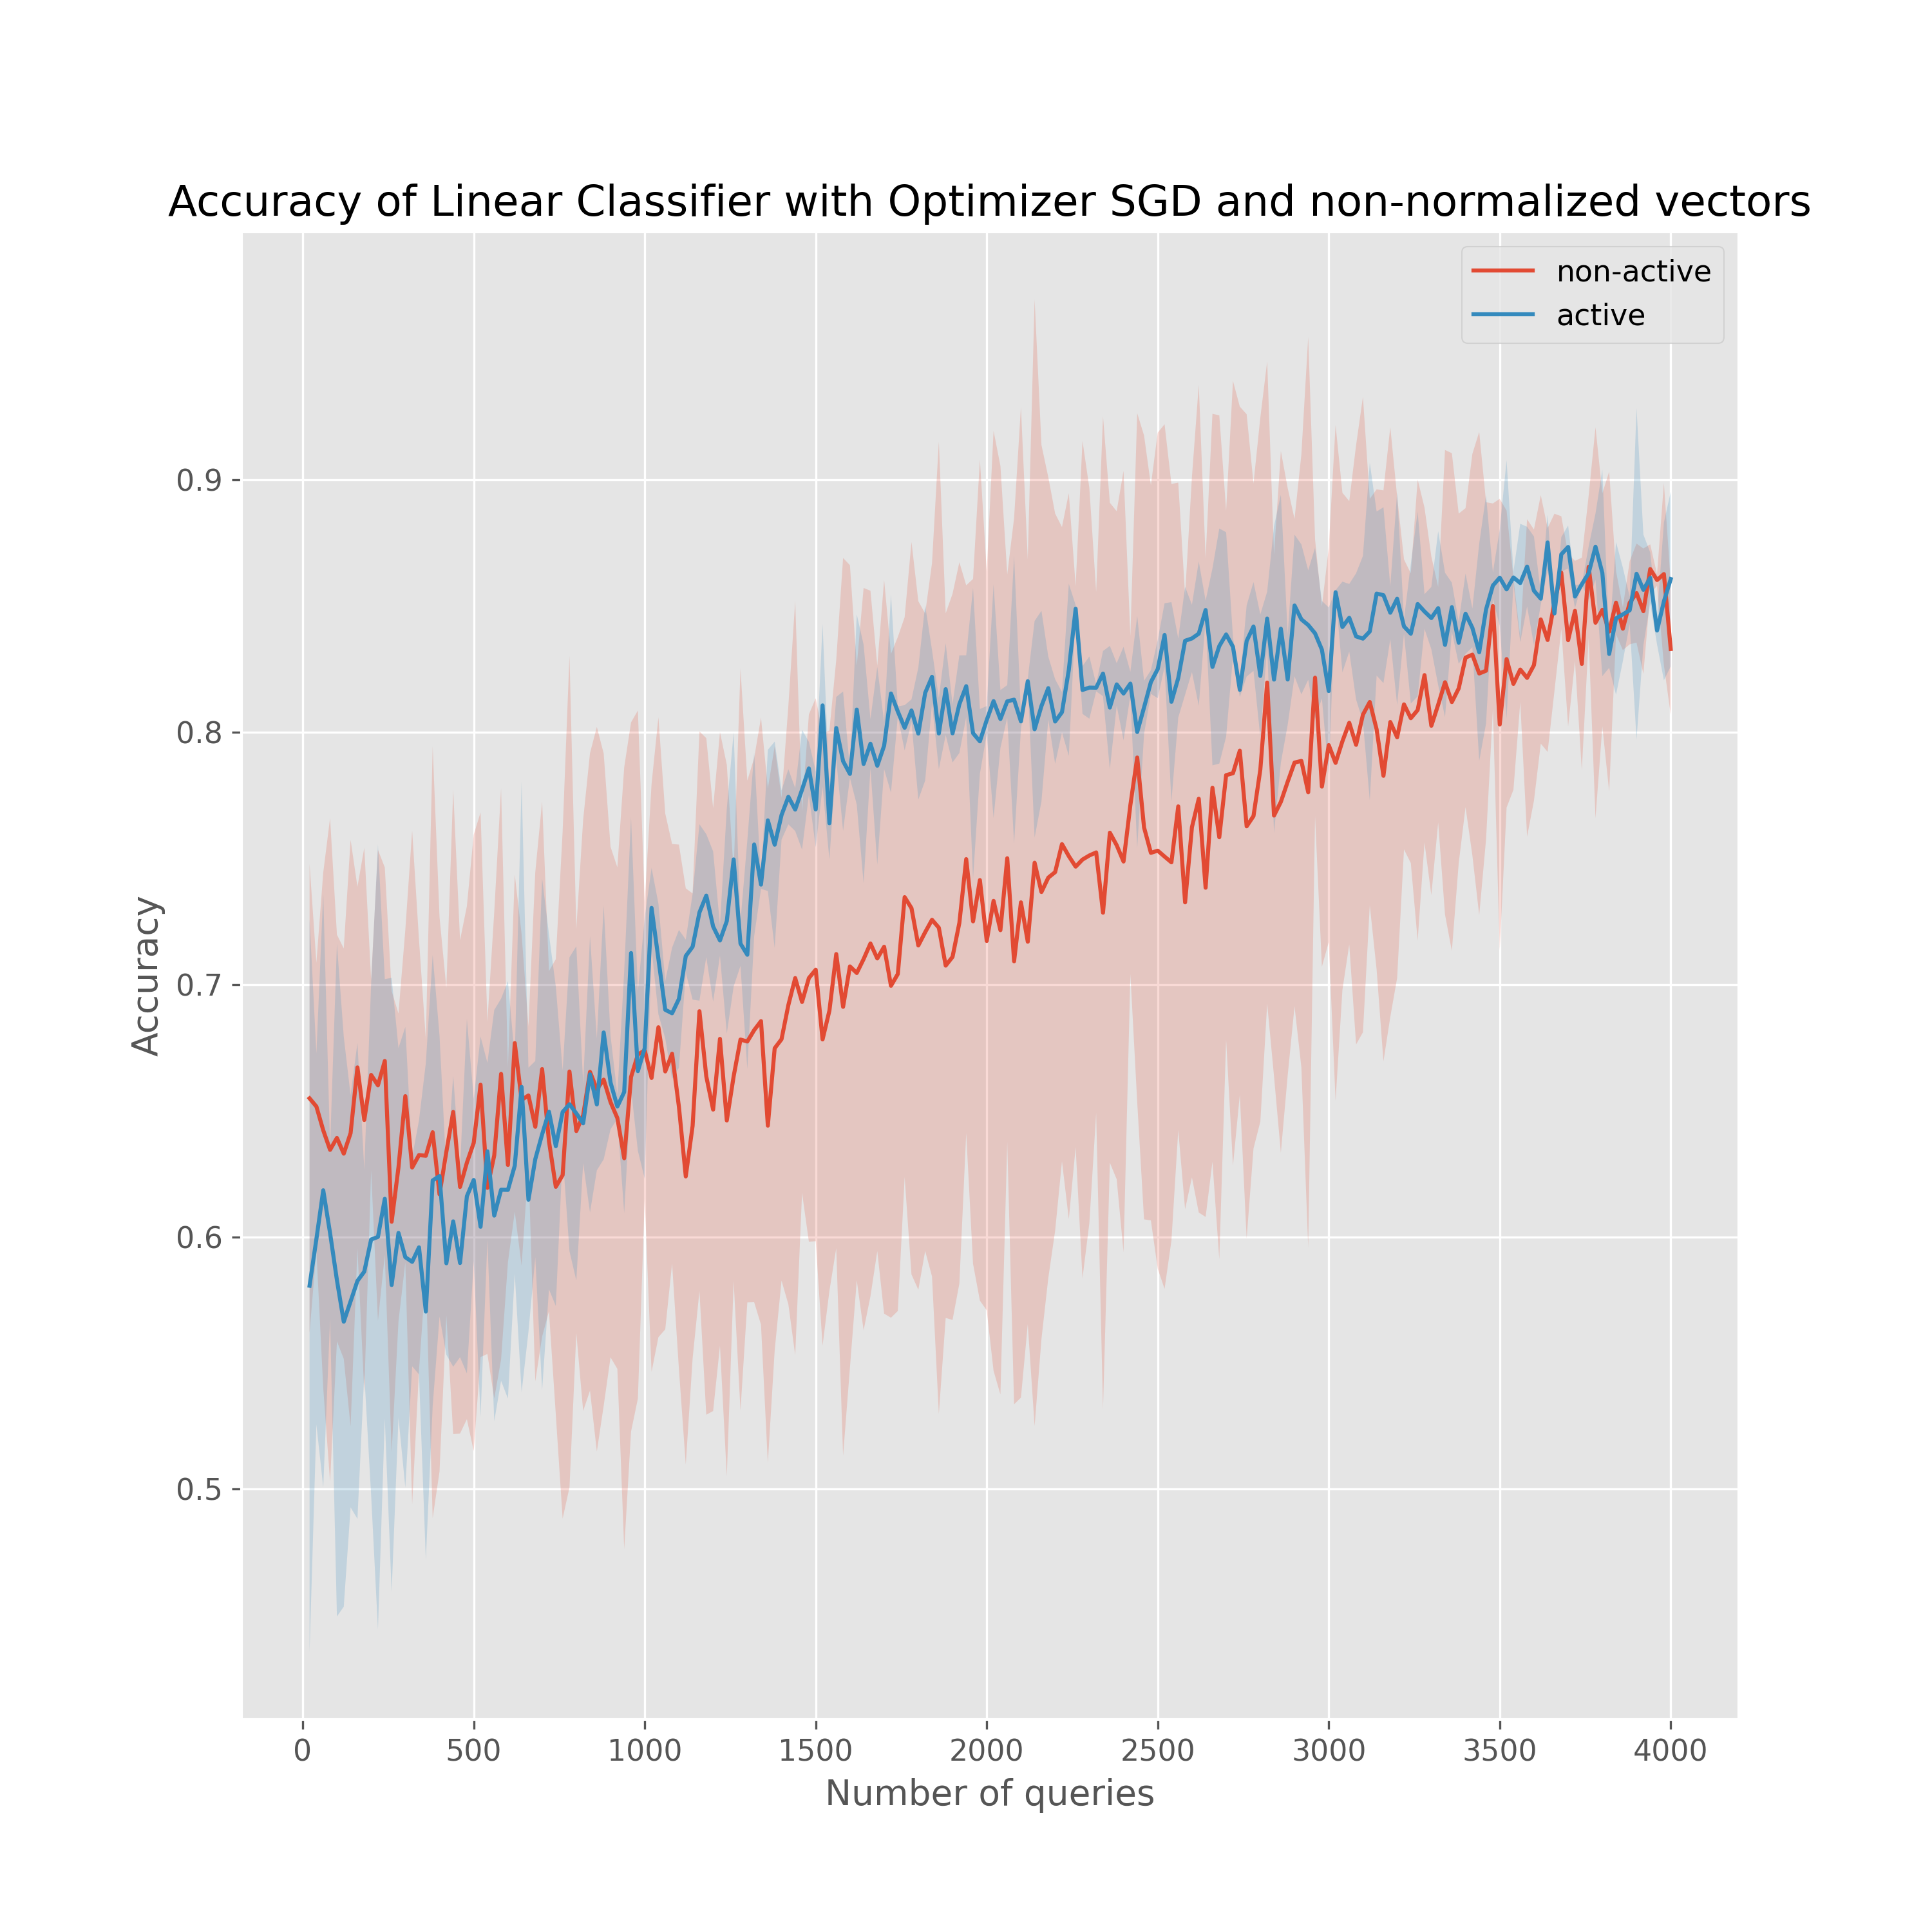
\includegraphics[width=\linewidth]{active-vs-base-moons-linear-loss-SGD-non-normalized-ci}
  \end{minipage}%
  \begin{minipage}{.45\textwidth}
    \centering
    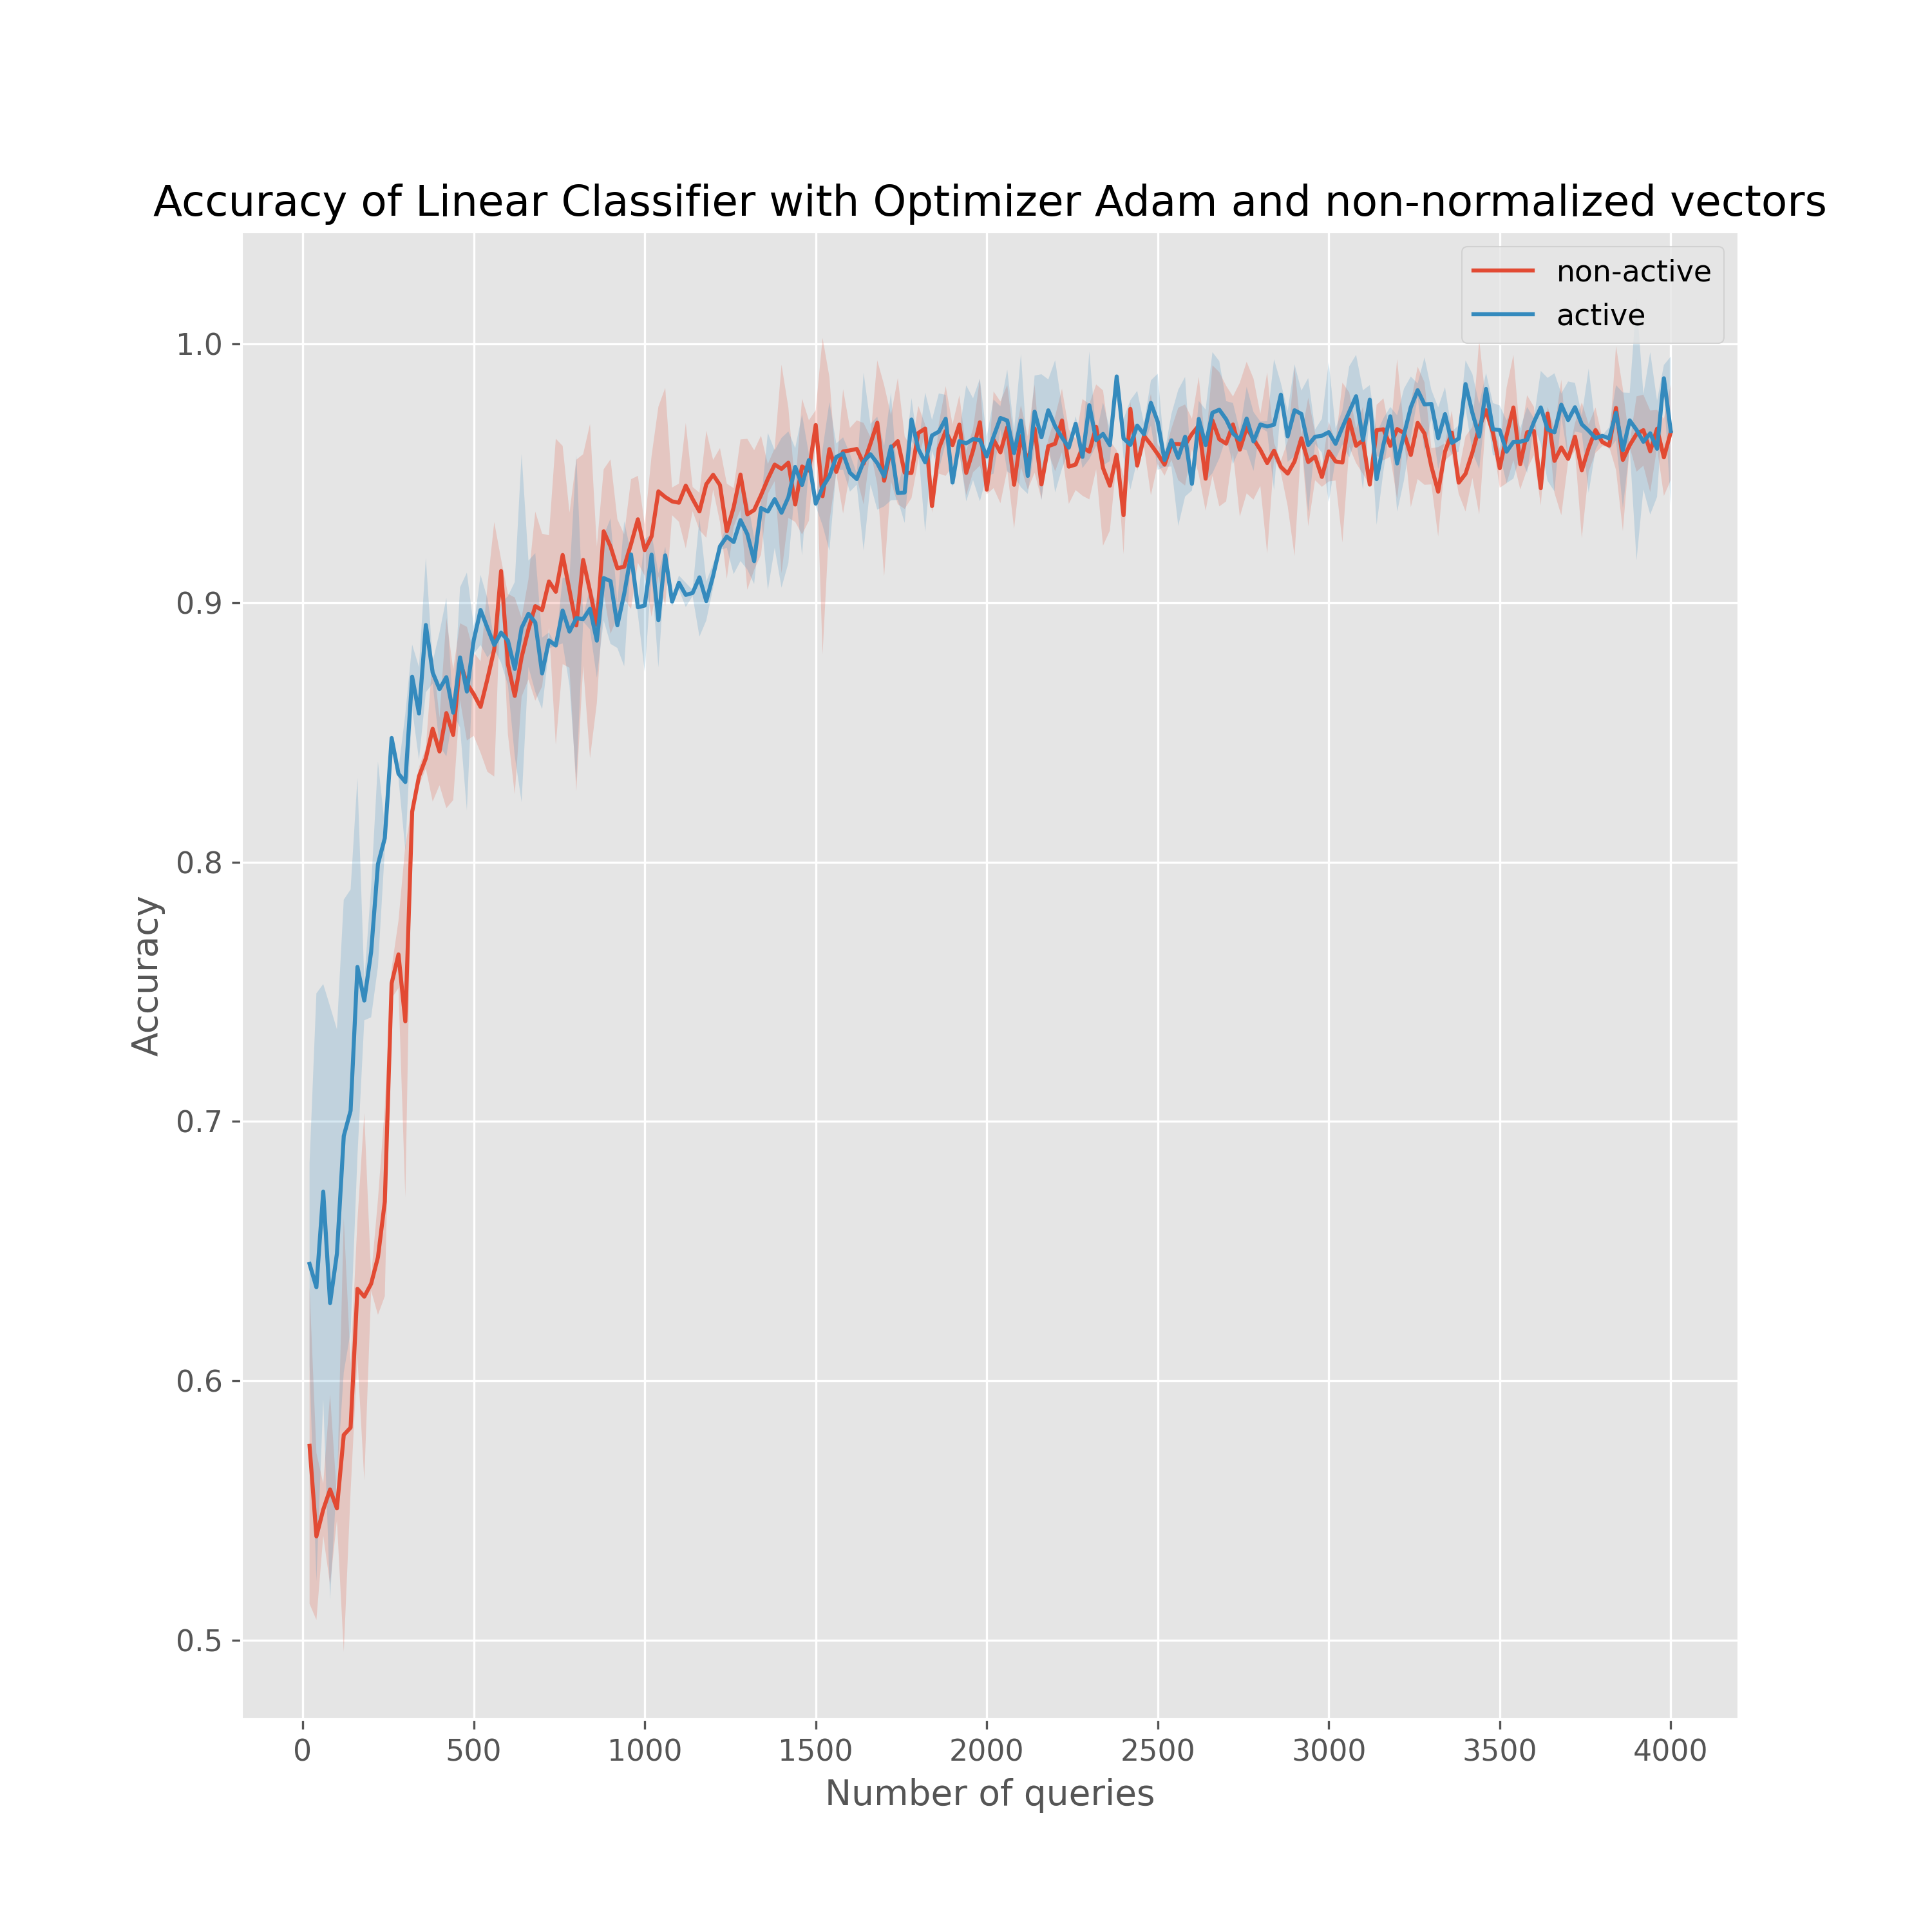
\includegraphics[width=\linewidth]{active-vs-base-moons-linear-loss-Adam-non-normalized-ci}
  \end{minipage}
  \caption{Performance SVM on non-normalized learned features SGD (left) vs Adam (right)}\label{fig:svm-non-normalized-ci}
\end{figure}

Clearly we see that on normalized version the performance of an active approach yields better results that non-active
but when normalized features are used we see that this effect almost disappears completely.
Moreover, using Adam reduces the difference between algorithms.

% add figures
\begin{figure}[h]
  \centering
  \begin{minipage}{.45\textwidth}
    \centering
    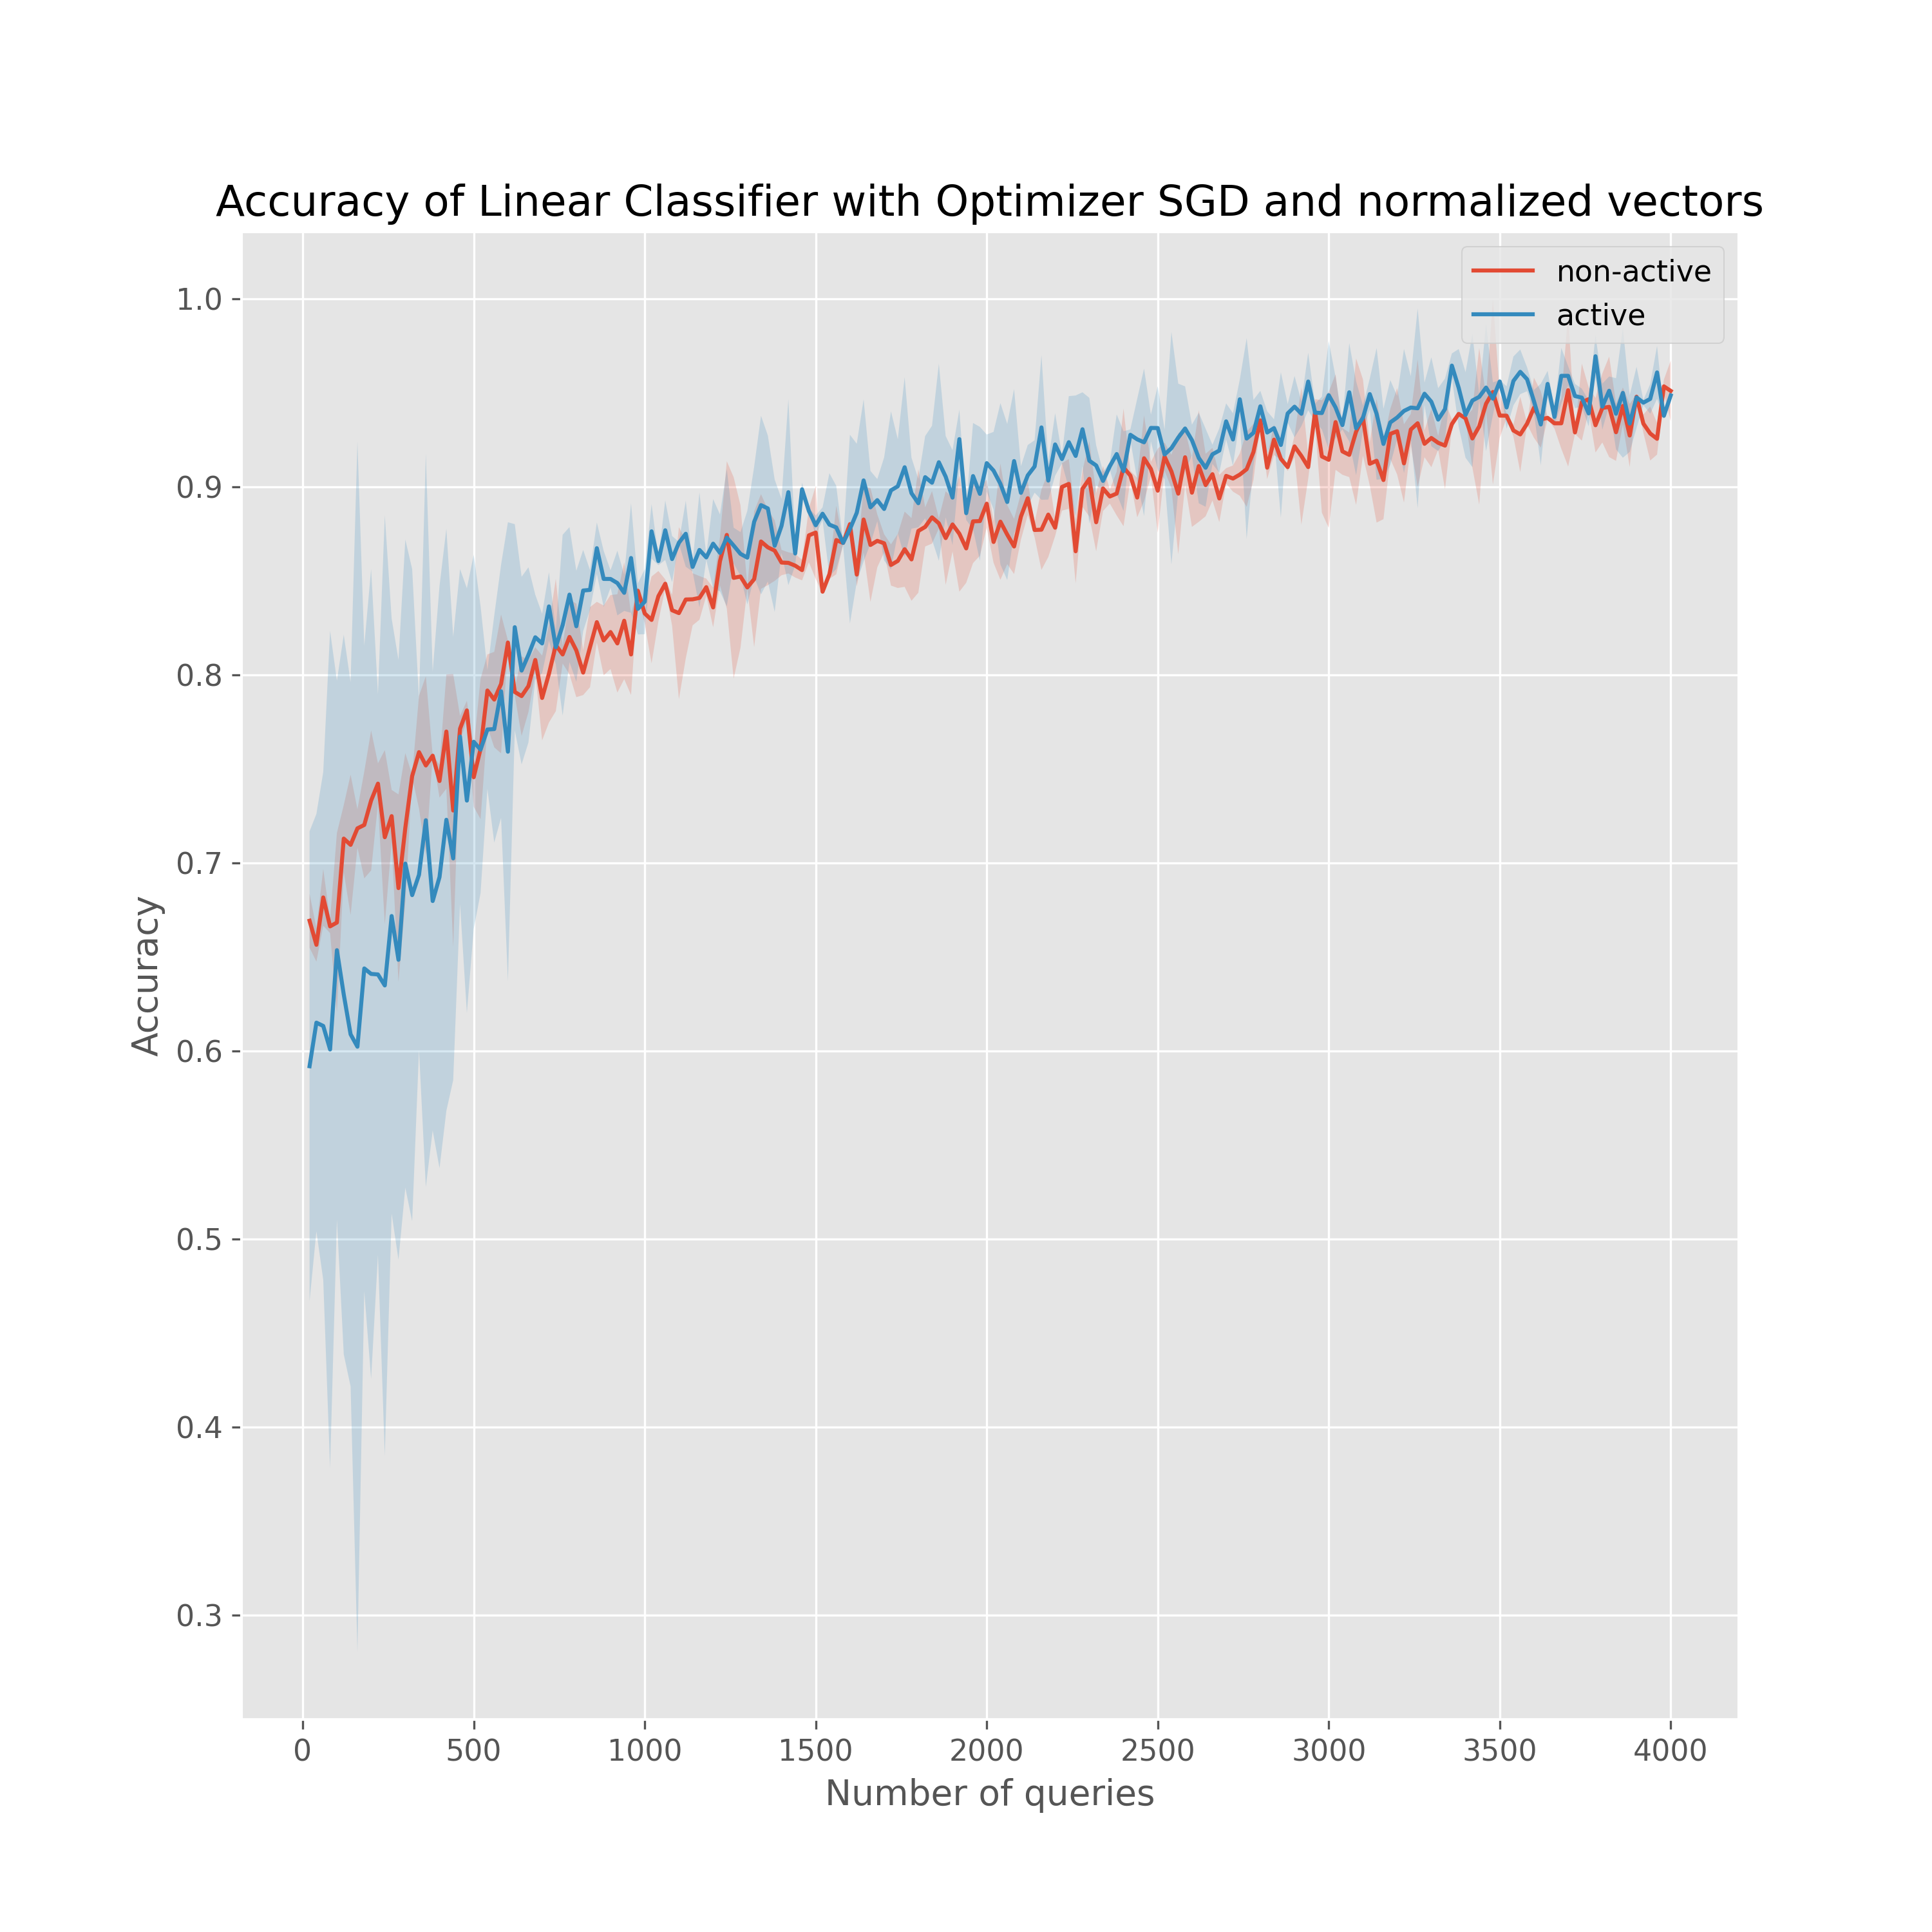
\includegraphics[width=\linewidth]{active-vs-base-moons-linear-loss-SGD-normalized-ci}
  \end{minipage}%
  \begin{minipage}{.45\textwidth}
    \centering
    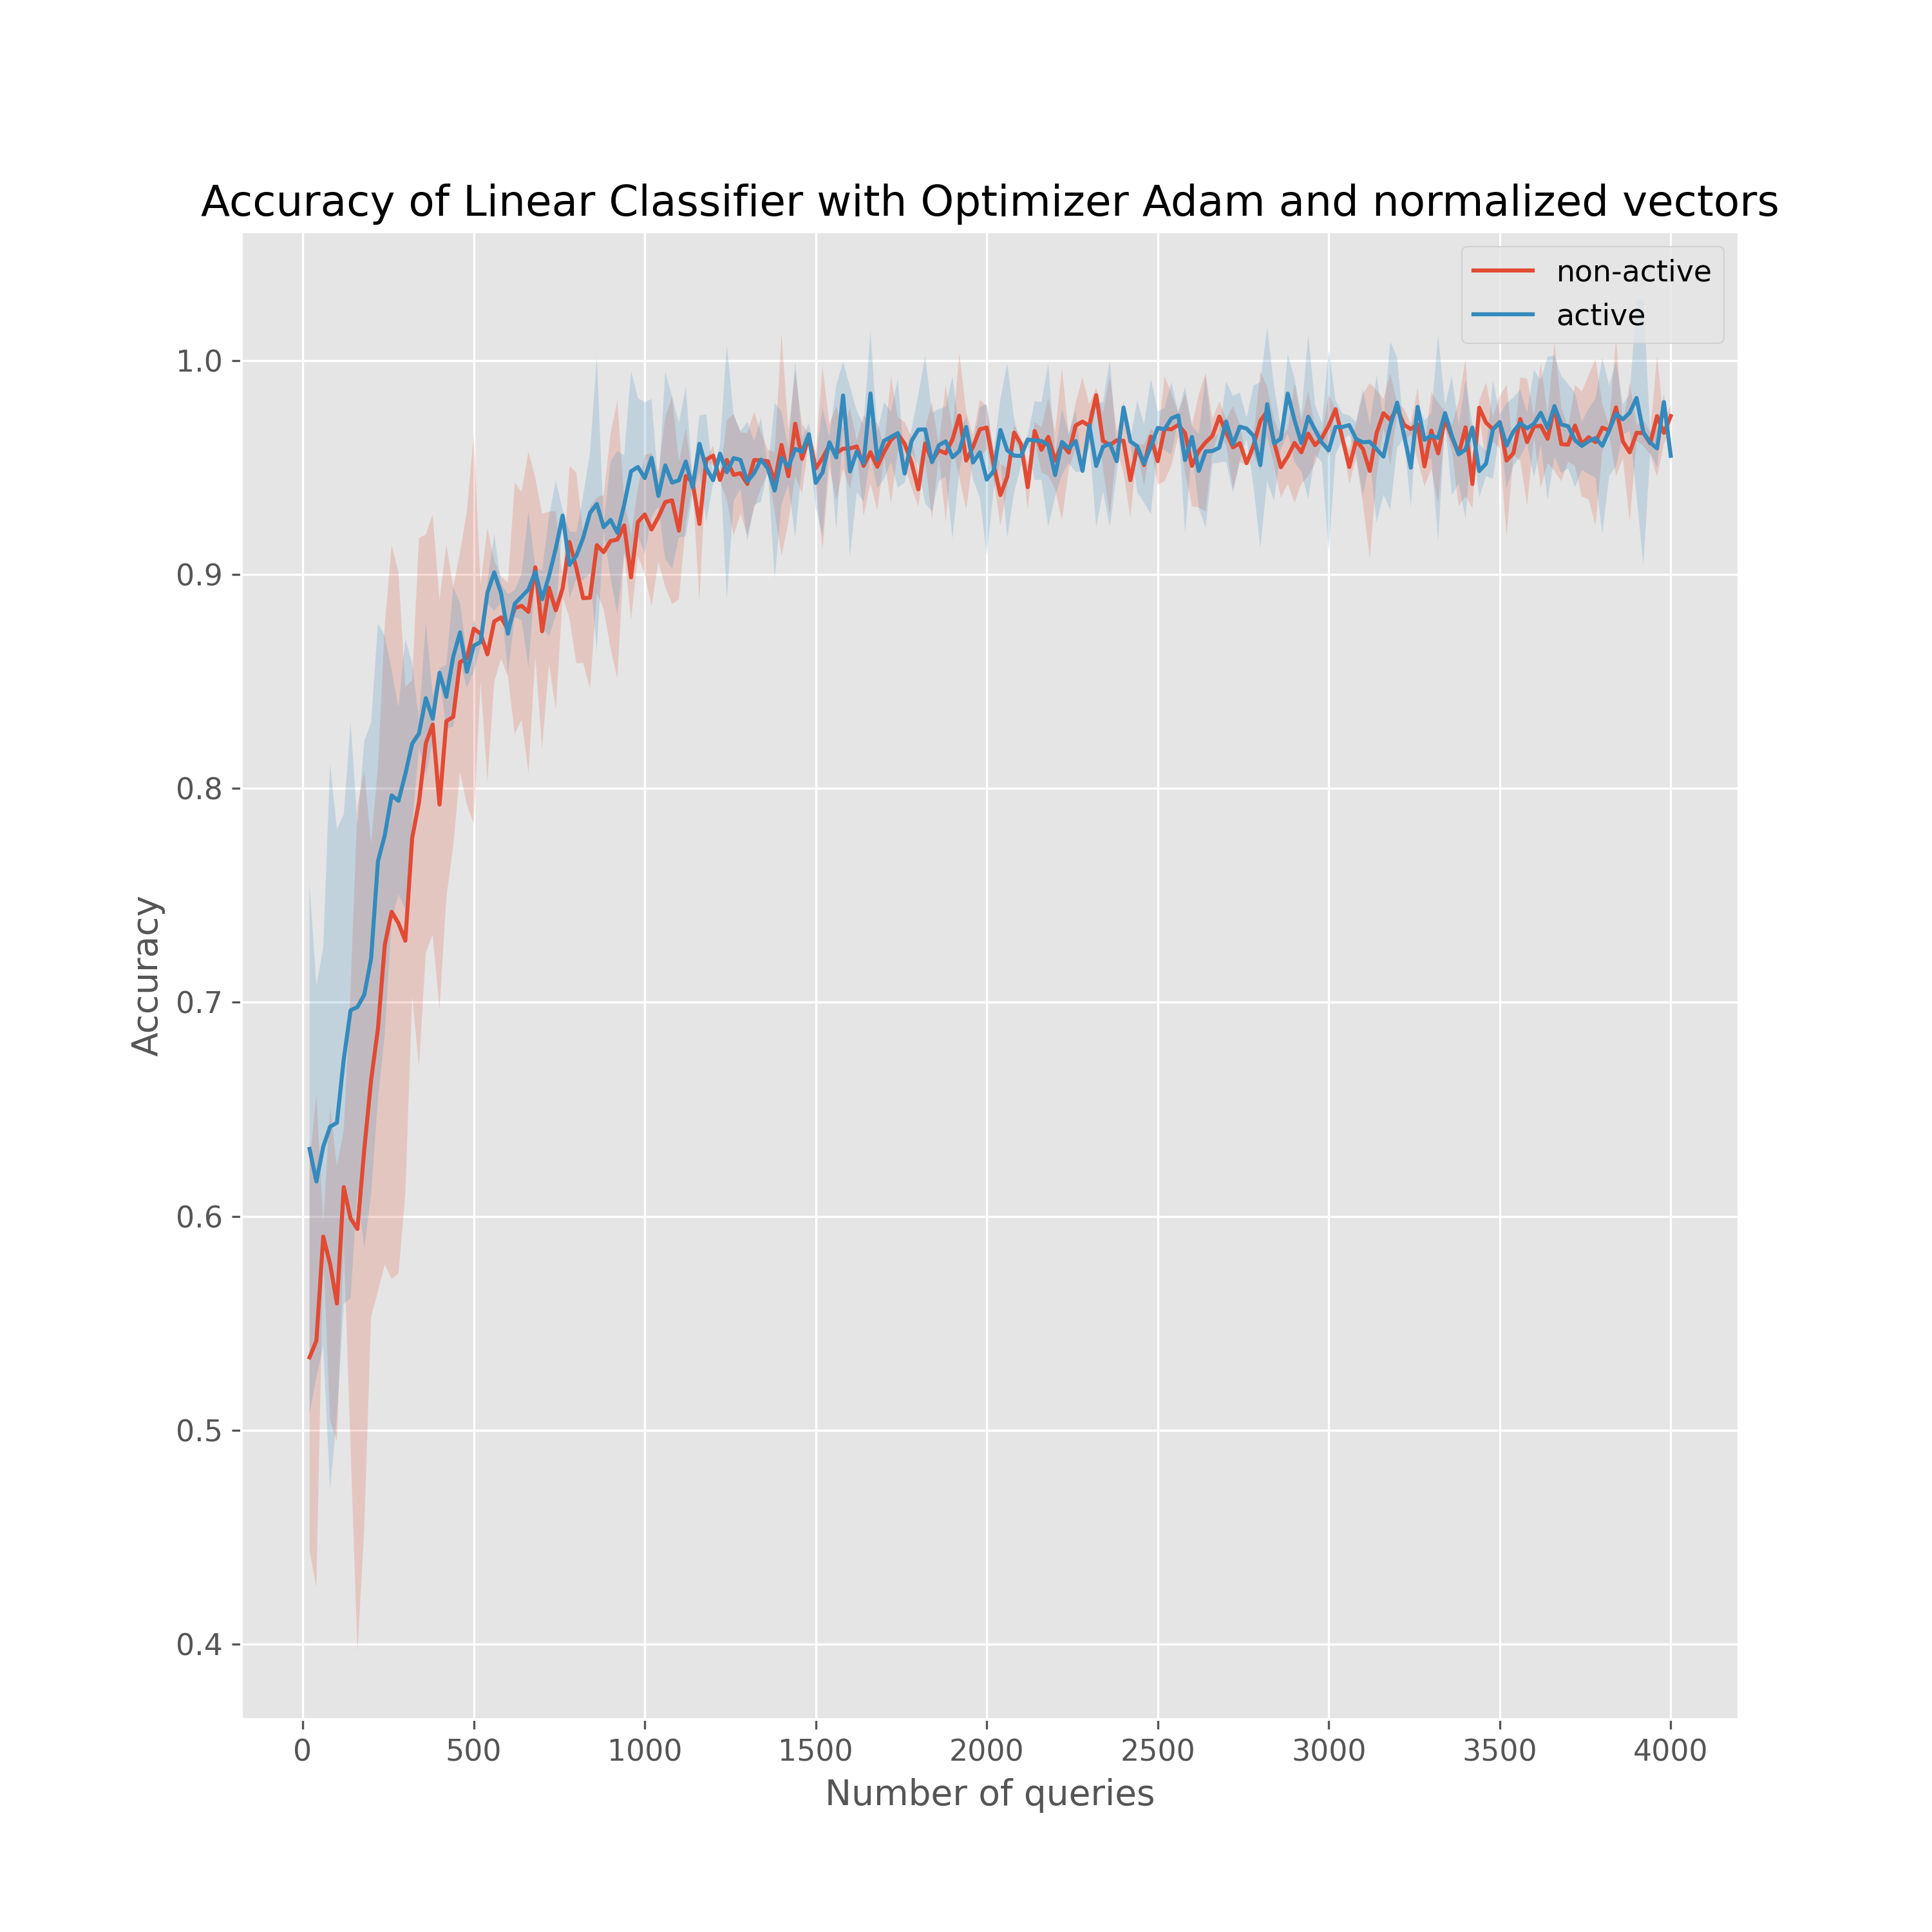
\includegraphics[width=\linewidth]{active-vs-base-moons-linear-loss-Adam-normalized-ci}
  \end{minipage}
  \caption{Performance SVM on normalized learned features SGD (left) vs Adam (right)}\label{fig:svm-normalized-ci}
\end{figure}


\subsection{Experiment 2: Comparison of $l_2$ loss through time of active algorithm}
Using the exact setup as in Experiment 1, we report the results of the $l_2$ loss through time for ActSim-NeuralUCB.
The results of this experiment are shown in figure (\ref{fig:l2-loss-non-normalized-ci}) and (\ref{fig:l2-loss-normalized-ci}).
\begin{figure}[!h]
  \centering
  \begin{minipage}{.45\textwidth}
    \centering
    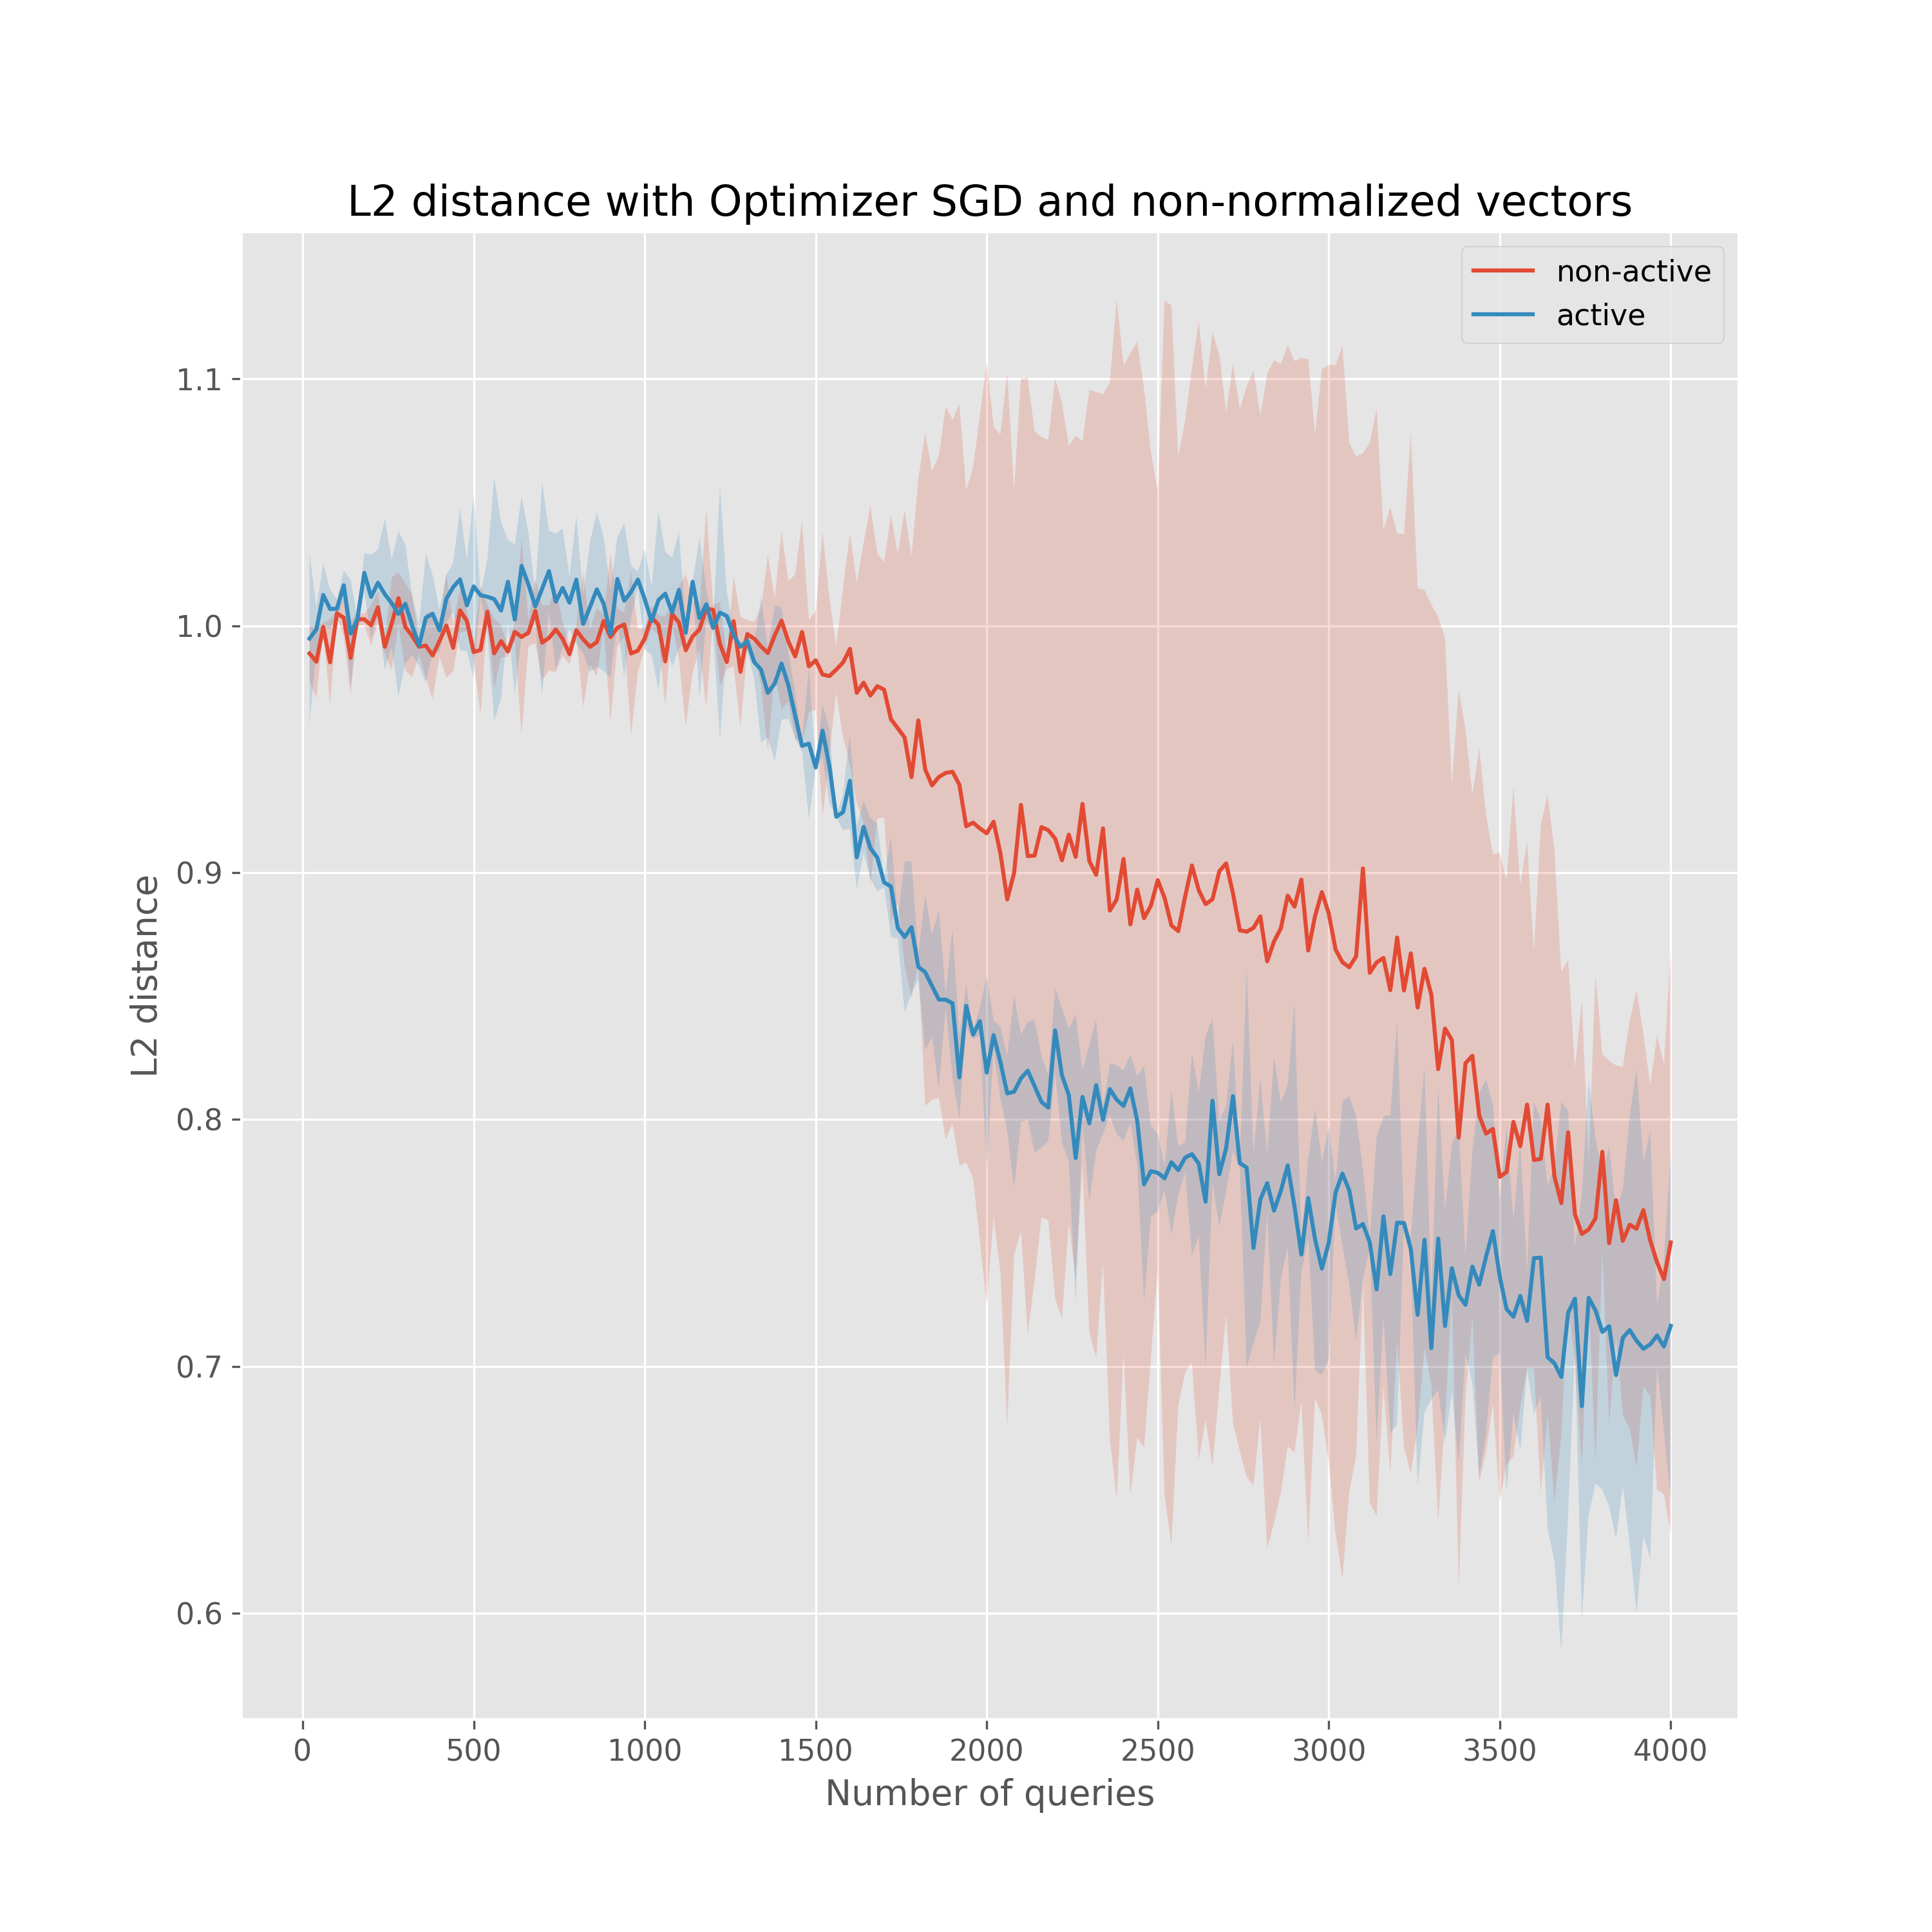
\includegraphics[width=\linewidth]{active-vs-base-moons-l2-loss-SGD-non-normalized-ci}
  \end{minipage}%
  \begin{minipage}{.45\textwidth}
    \centering
    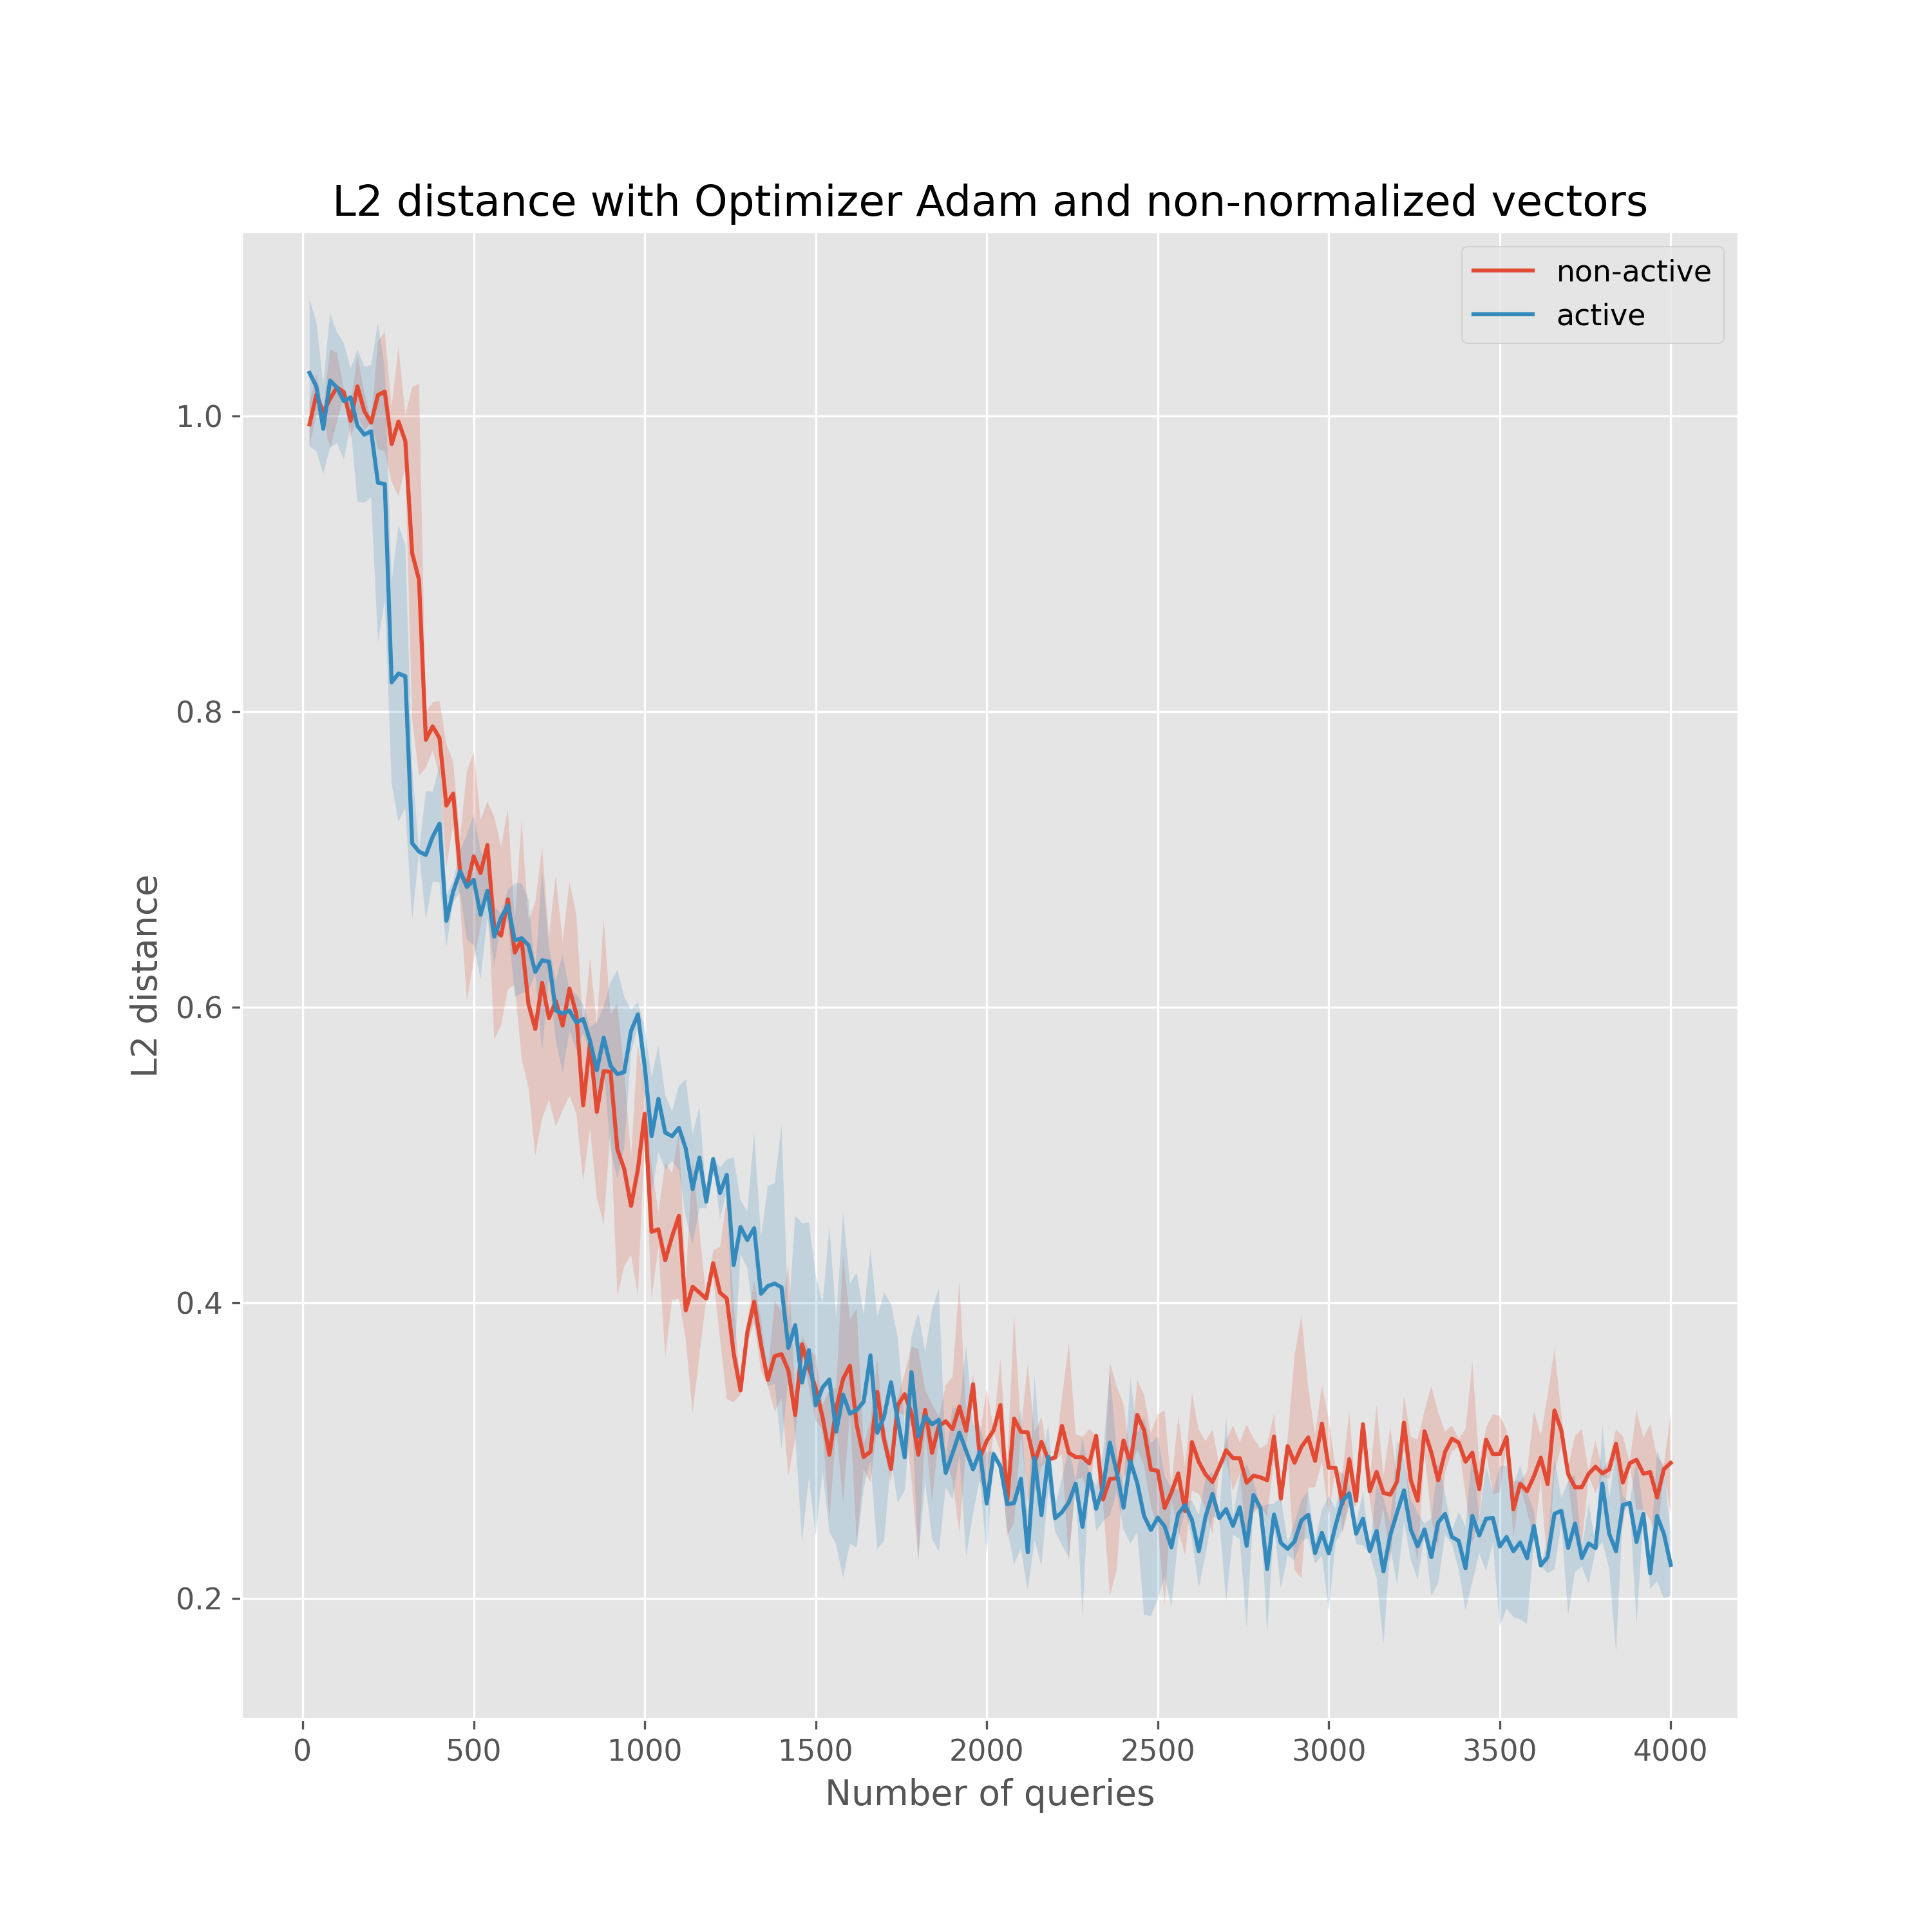
\includegraphics[width=\linewidth]{active-vs-base-moons-l2-loss-Adam-non-normalized-ci}
  \end{minipage}
  \caption{$l_2$ loss on non-normalized features SGD (left) vs Adam (right)}\label{fig:l2-loss-non-normalized-ci}
\end{figure}

% add figures
\begin{figure}[t]
  \centering
  \begin{minipage}{.45\textwidth}
    \centering
    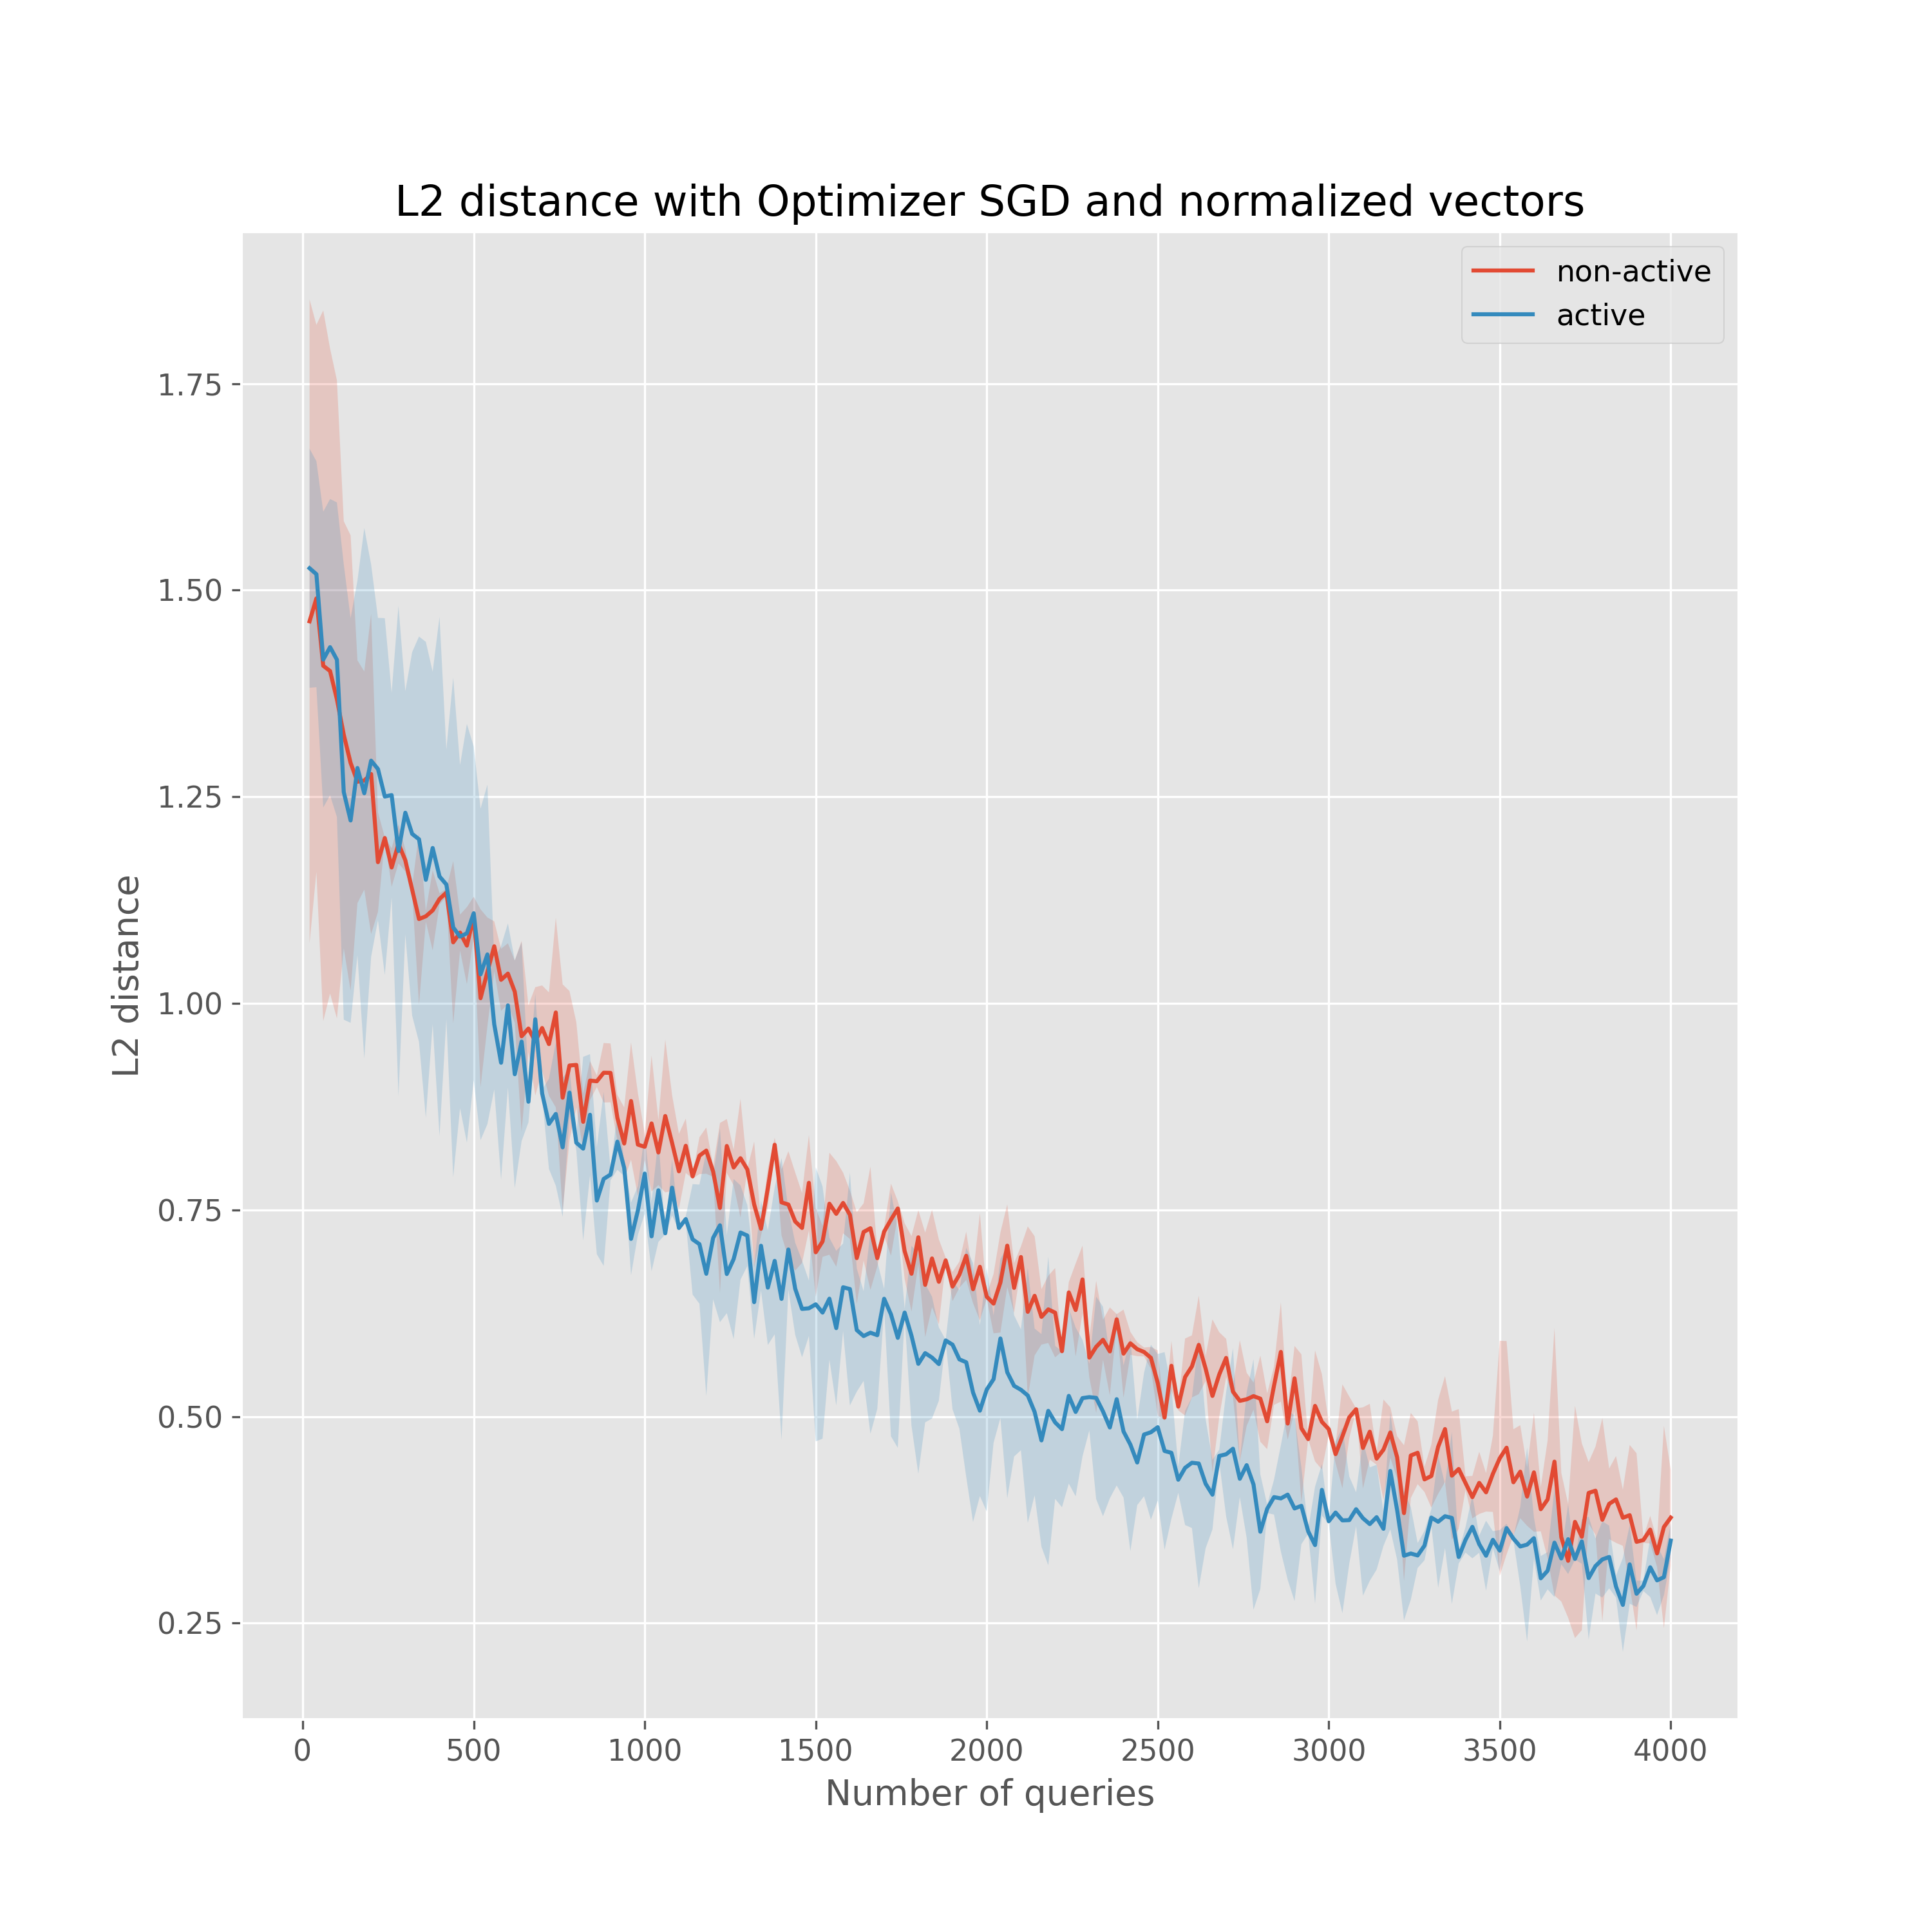
\includegraphics[width=\linewidth]{active-vs-base-moons-l2-loss-SGD-normalized-ci}
  \end{minipage}%
  \begin{minipage}{.45\textwidth}
    \centering
    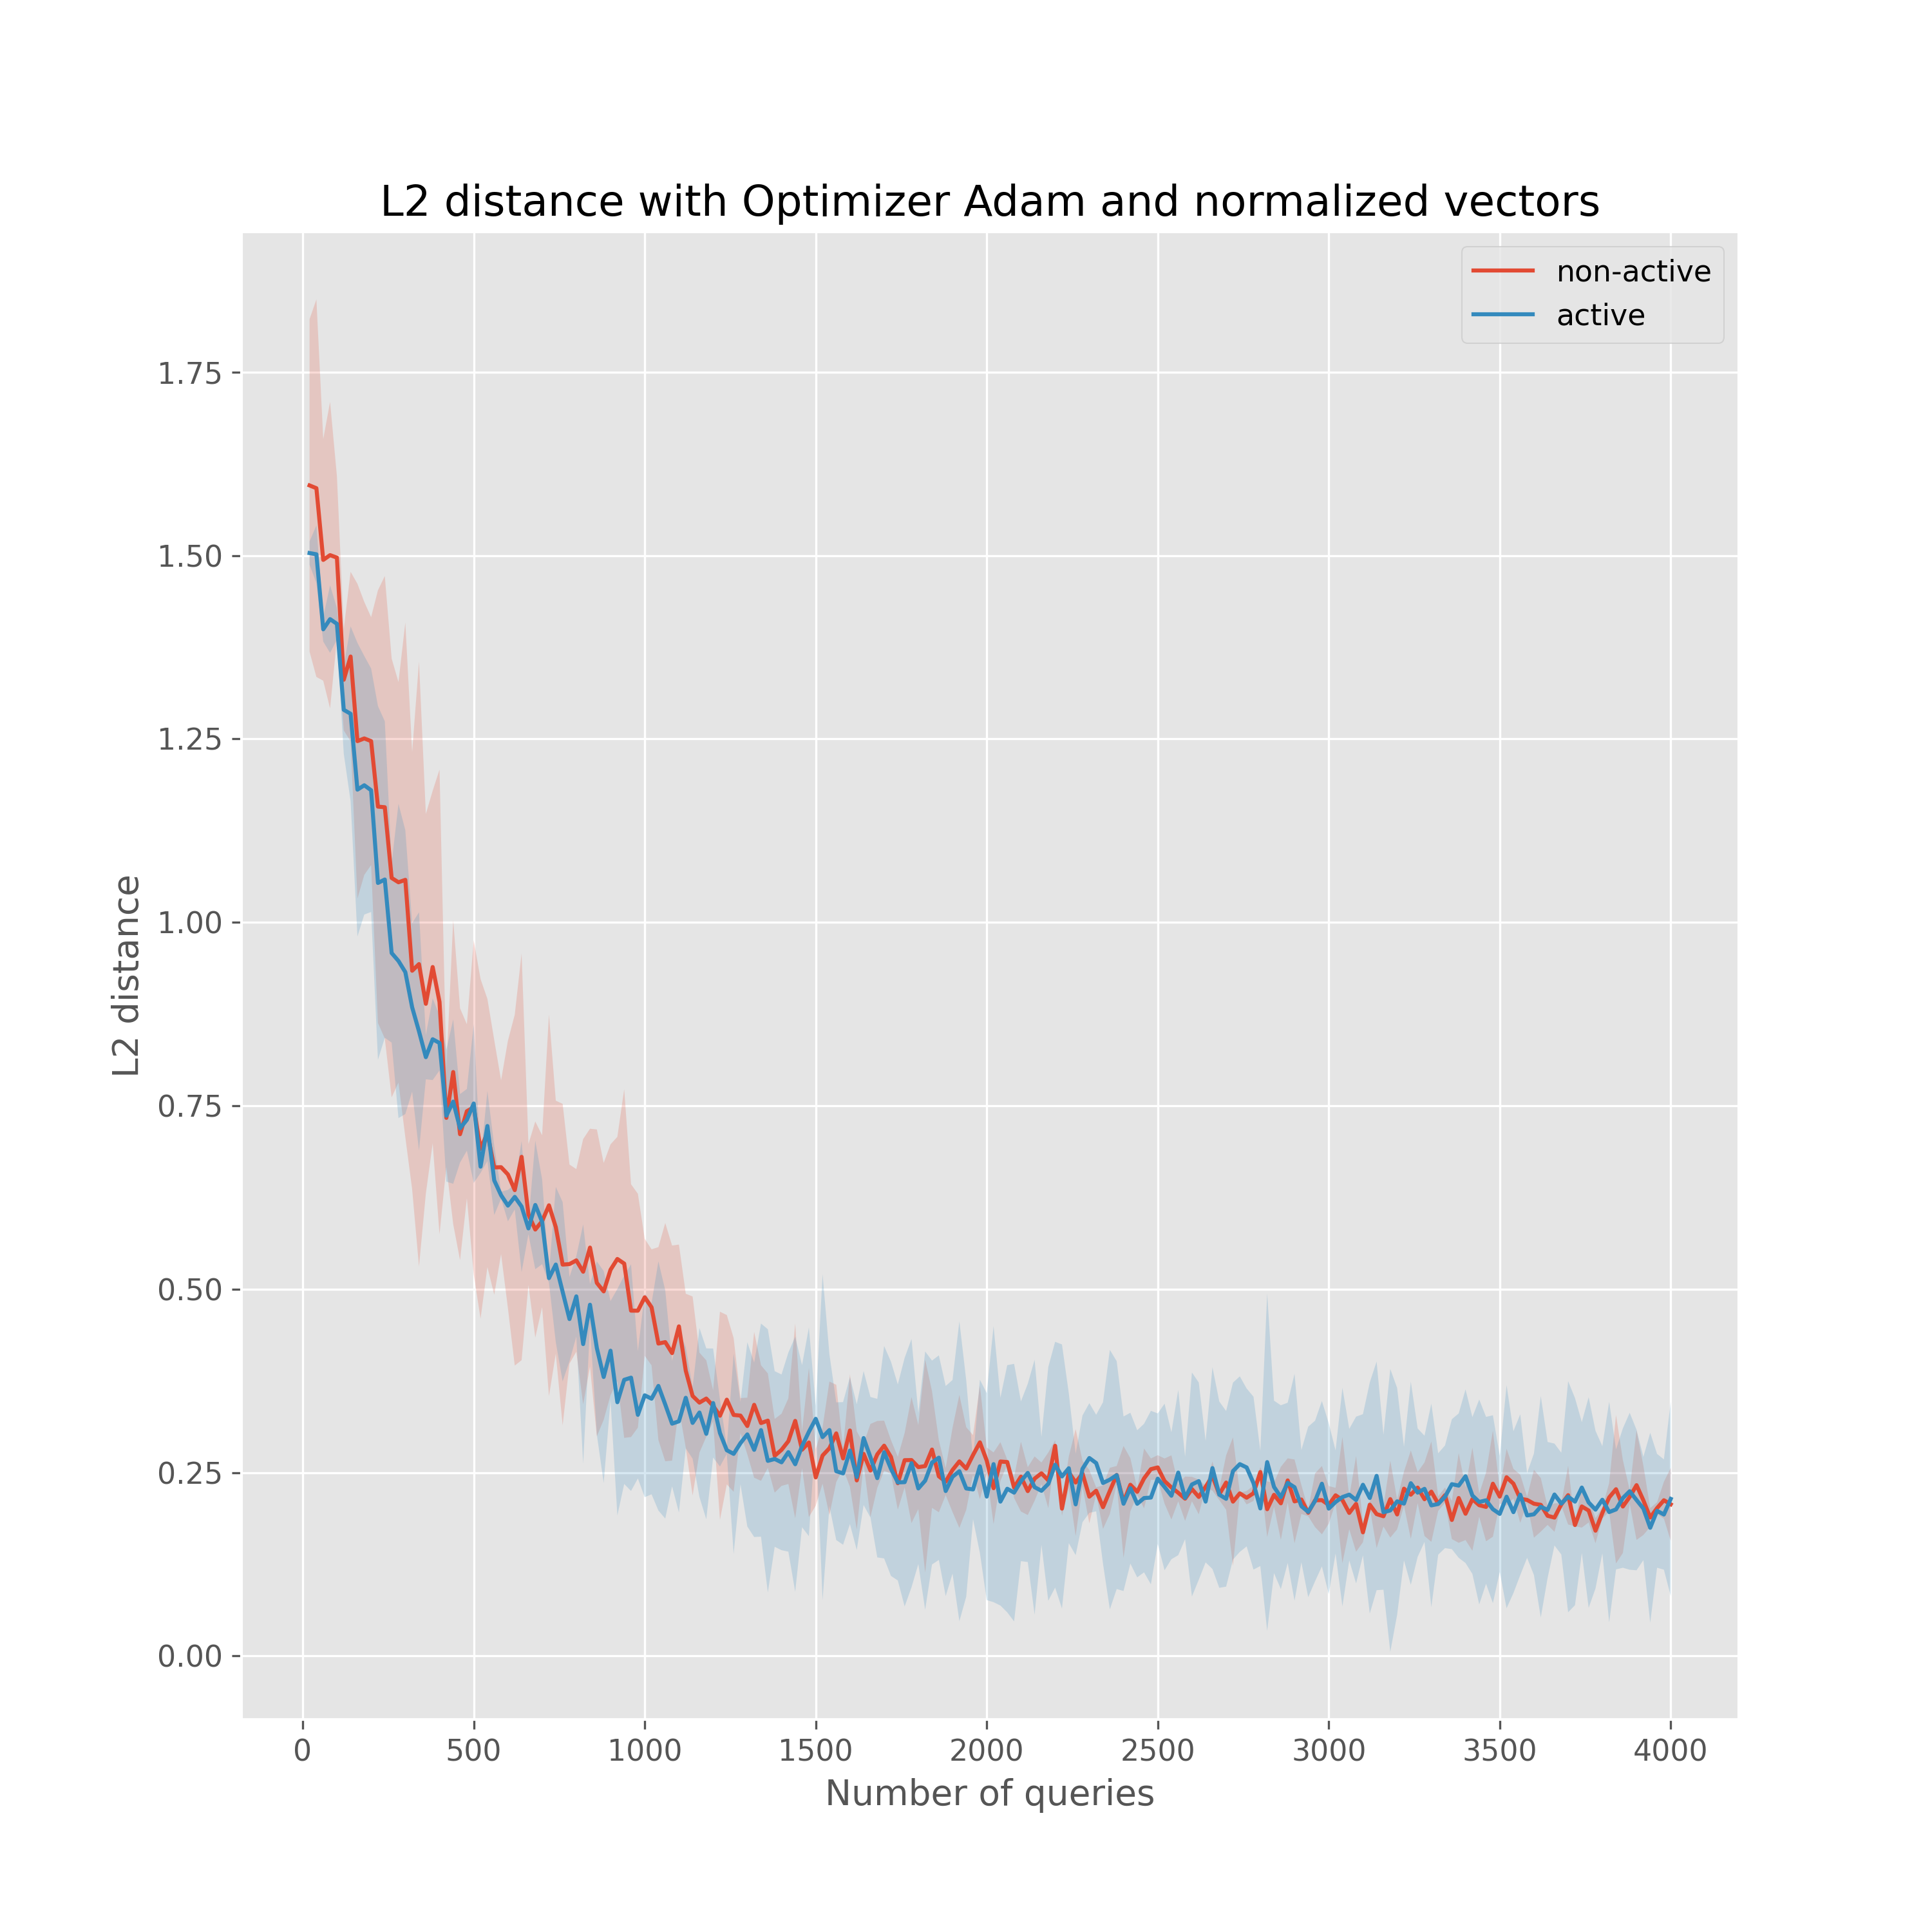
\includegraphics[width=\linewidth]{active-vs-base-moons-l2-loss-Adam-normalized-ci}
  \end{minipage}
  \caption{$l_2$ loss on normalized features SGD (left) vs Adam (right)}\label{fig:l2-loss-normalized-ci}
\end{figure}
As before, we observe that adam erases to a large extent the differences between algorithms and that the performance
of the active approach depends heavily on the particular optimizer used.

\subsection{Experiment 3: Regret of OnSim-NeuralUCB}
We observe the performance of OnSim-NeuralUCB by compring the regret of the algorithm with the regret of an epsilon-greedy
neural network with the same architecture and hyperparameters. We report the results only for Adam as it had a significantly better performance,
but provide the comparison both for the normalized and unormalized versions.
Like in the previous experiment all graphs contain the mean and a 95\% confidence interval over 10 runs.
 We also compare various values for the exploration parameter. The results can be found in figure (\ref{fig:online-epsilon-vs-neural-ci})

% add figures
\begin{figure}[!h]
  \centering
  \begin{minipage}{.45\textwidth}
    \centering
    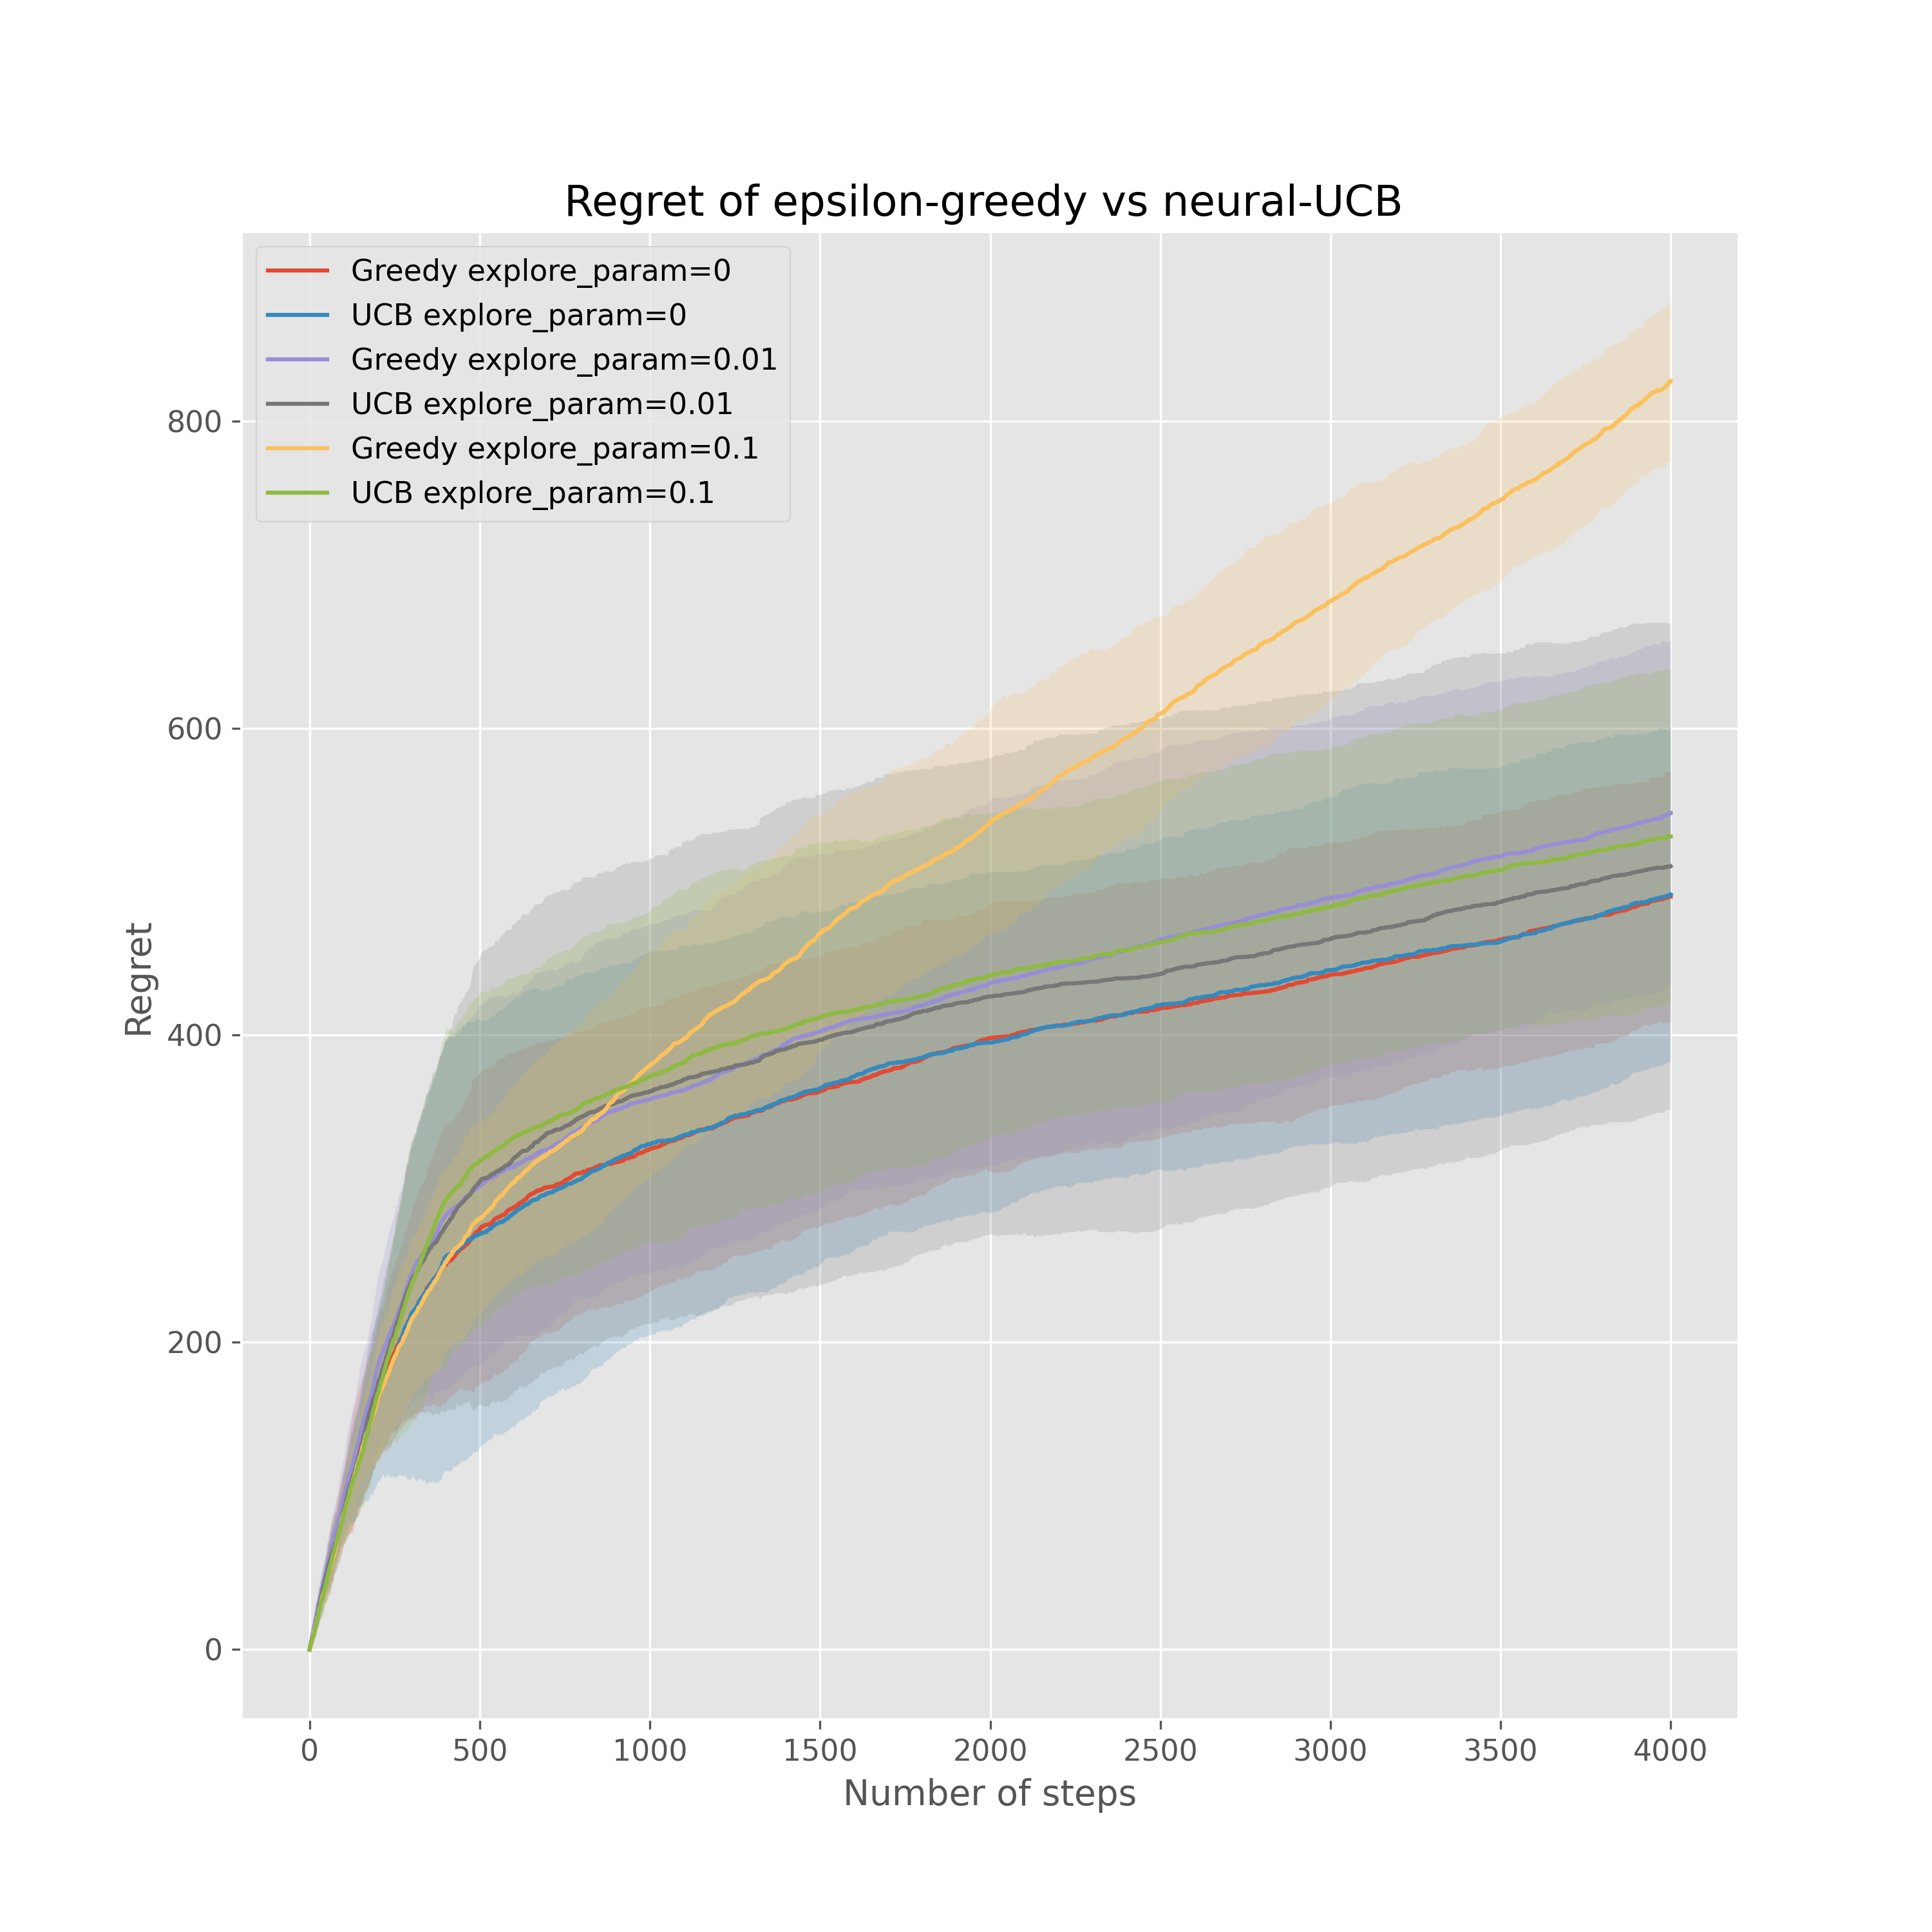
\includegraphics[width=\linewidth]{online-epsilon-vs-neural-reduced-nonormalized-ci}
  \end{minipage}%
  \begin{minipage}{.45\textwidth}
    \centering
    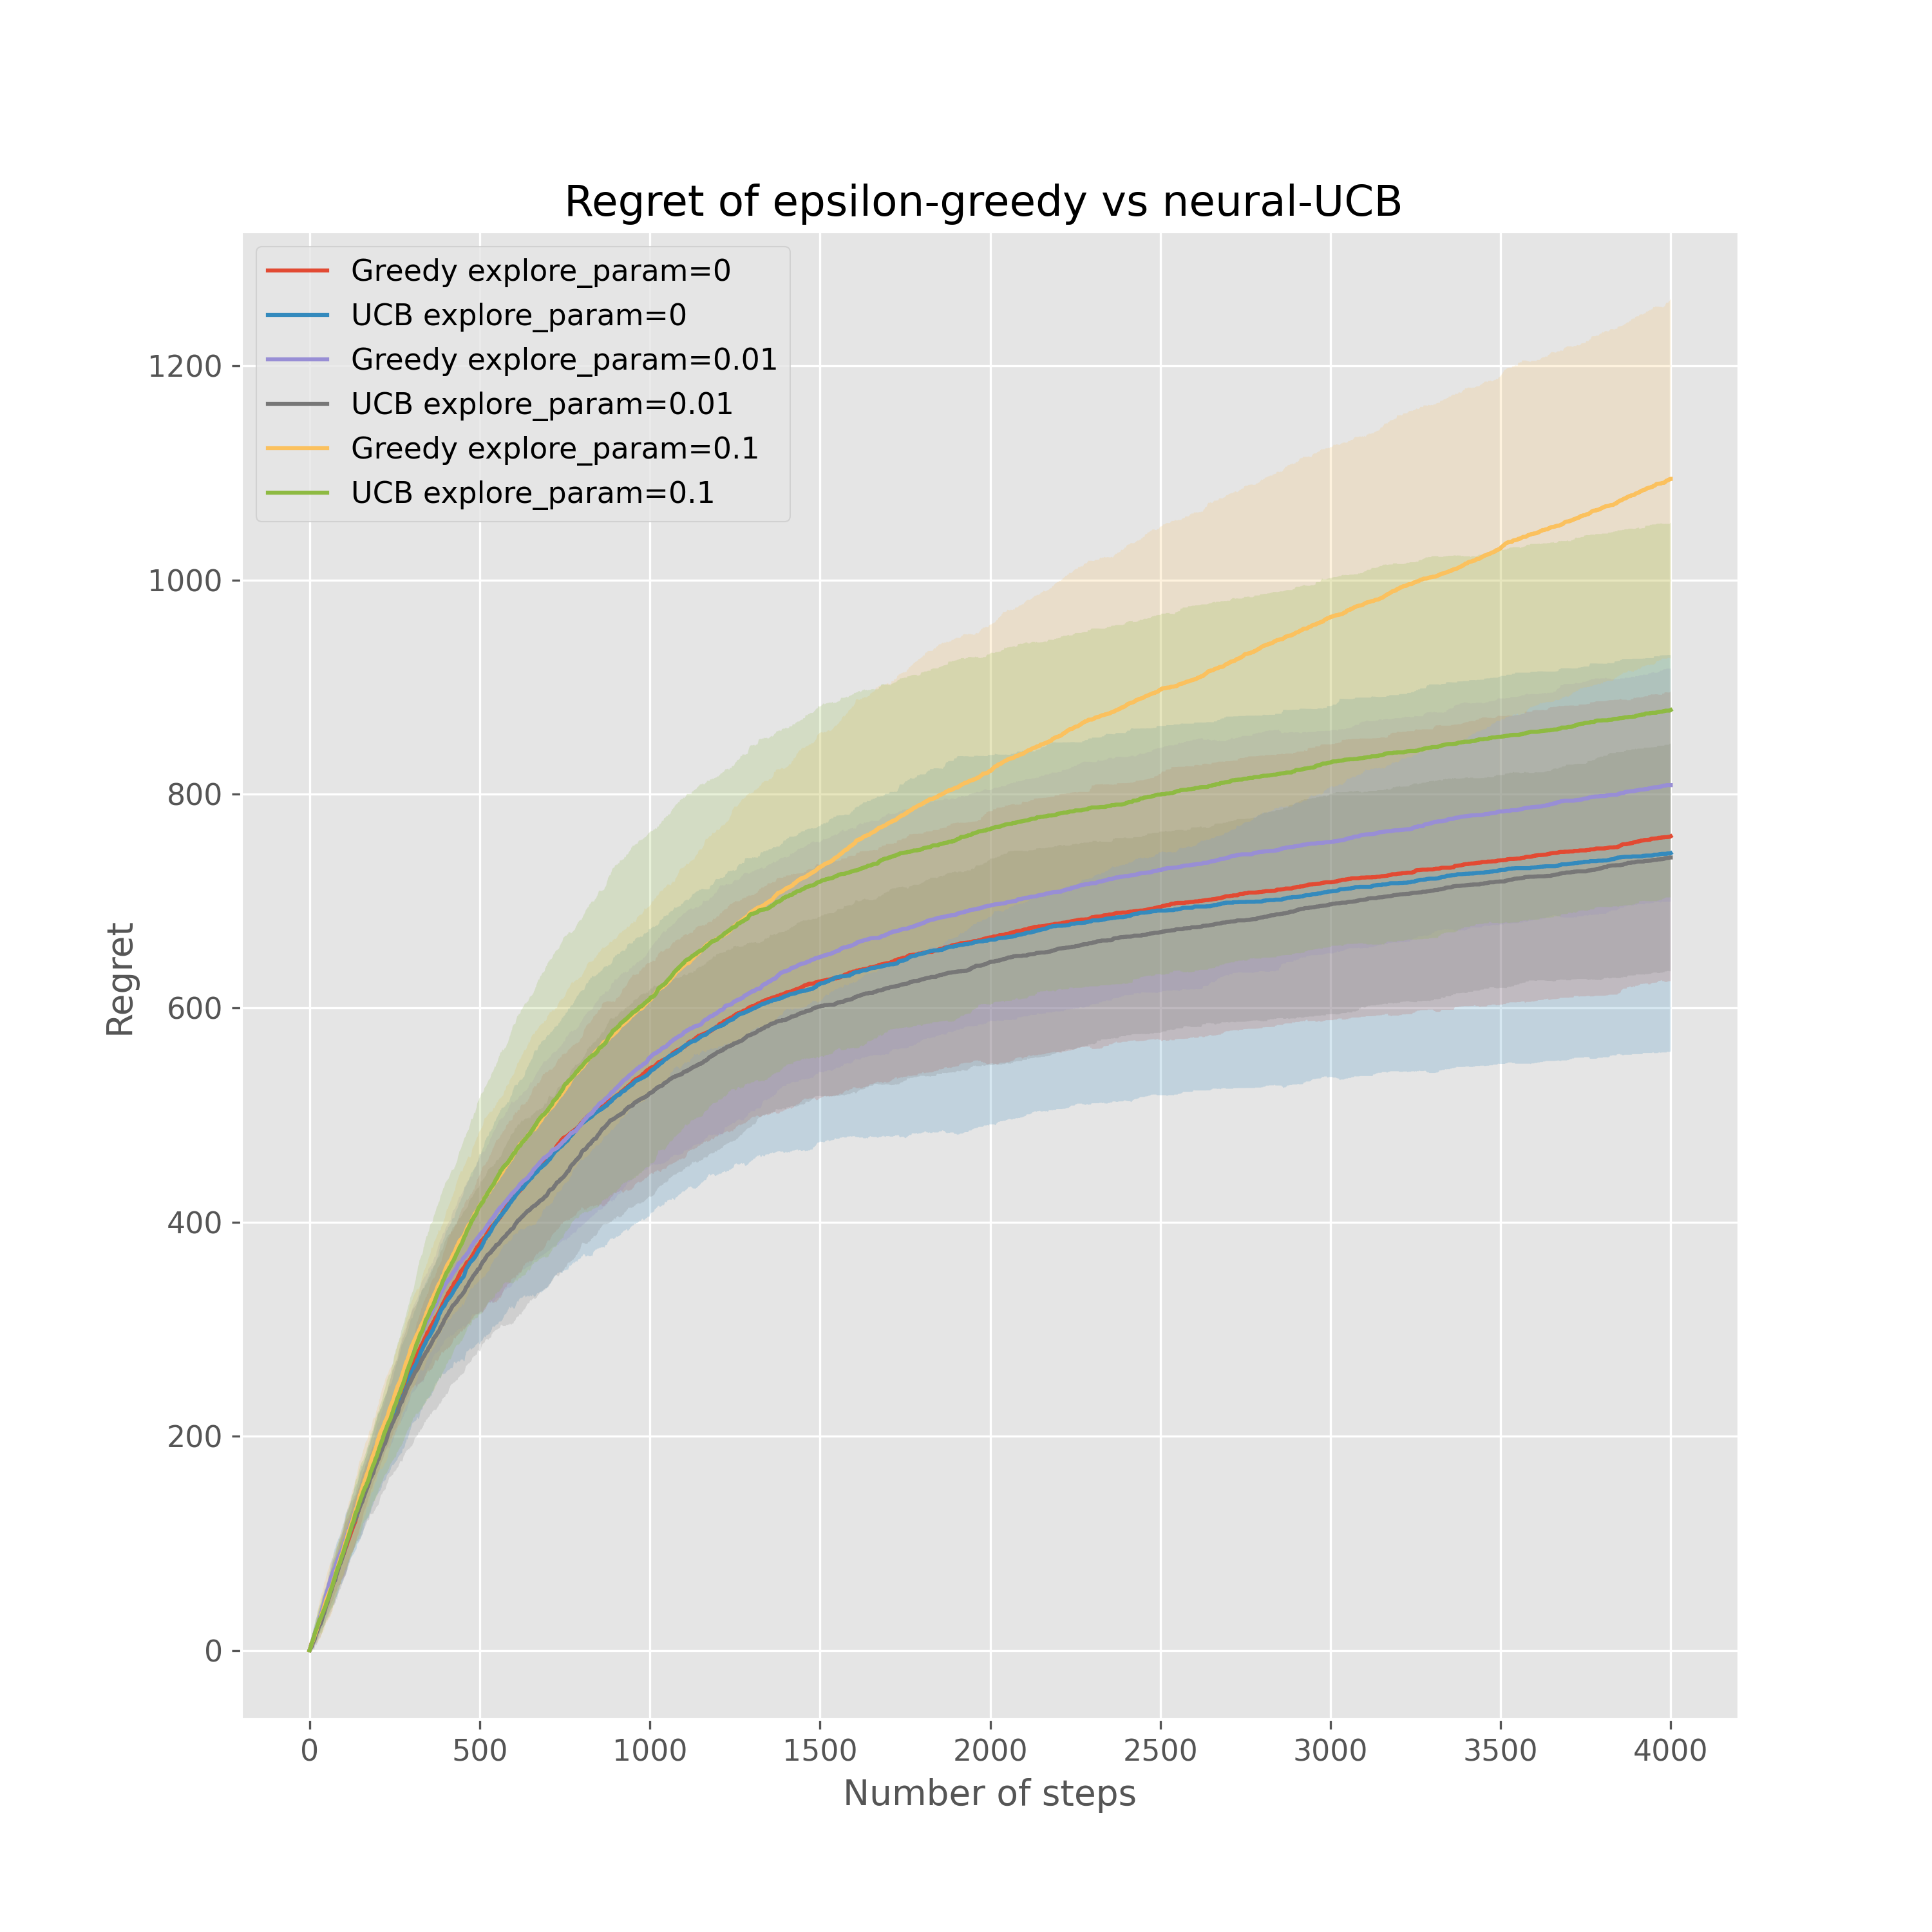
\includegraphics[width=\linewidth]{online-epsilon-vs-neural-reduced-normalized-ci}
  \end{minipage}
  \caption{Performance OnSim-NeuralUCB on non-normalized and normalized features}\label{fig:online-epsilon-vs-neural-ci}
\end{figure}

For this dataset we observe that there is no sigficant difference between using a simpler epsilon greedy approach
and our neural-ucb  based approach.
\subsection{LinearUCB}
\subparagraph{Dataset:}
To test the linear version of our algorithm we created a blobs dataset.
Every point is drawn from the following process. Assume that $x_i' \sim \mathcal{N}((0, 0)^\top,I_2)$ and $p_i \sim \text{Bernoulli}(p)$ where $p$ is
some parameter.
Then the data point $x_i$ is drawn as
\[x_i = \begin{bmatrix} 3 & 0\\ 0 & 1\\ \end{bmatrix} x_i' -(1-p_i)
\begin{bmatrix}
1\\
1\\
\end{bmatrix}
+ p_i
\begin{bmatrix}
1\\
0\\
\end{bmatrix}
\]
which corresponds to two blobs one placed on the left axis and one on the right axis.
We say that two points are similar if they share the same value of $p$.
We refer to this dataset as the Blobs dataset.



\subsubsection{Experiment 1: Effectiveness of active learning balanced and unbalanced datset}
We test the effectiveness of active learning on the balanced and unbalanced datasets.
For the unbalanced instance we use $p = 0.1$ but provide the results of an $l_2$ loss assuming that the real distribution of the data is balanced.
This is done to simulate a situation in which our collected unlabeled data is unbalanced and to show the improvement in robustness of the
algorithm. The plots in (\ref{fig:linucb-blobs-l2-loss-balanced}) and (\ref{fig:linucb-blobs-l2-loss-unbalanced})  contain the mean and the 95\% confidence interval for the
regret over 30 runs of each algorithm.

\begin{figure}[!h]
  \centering
  \begin{minipage}{.45\textwidth}
    \centering
    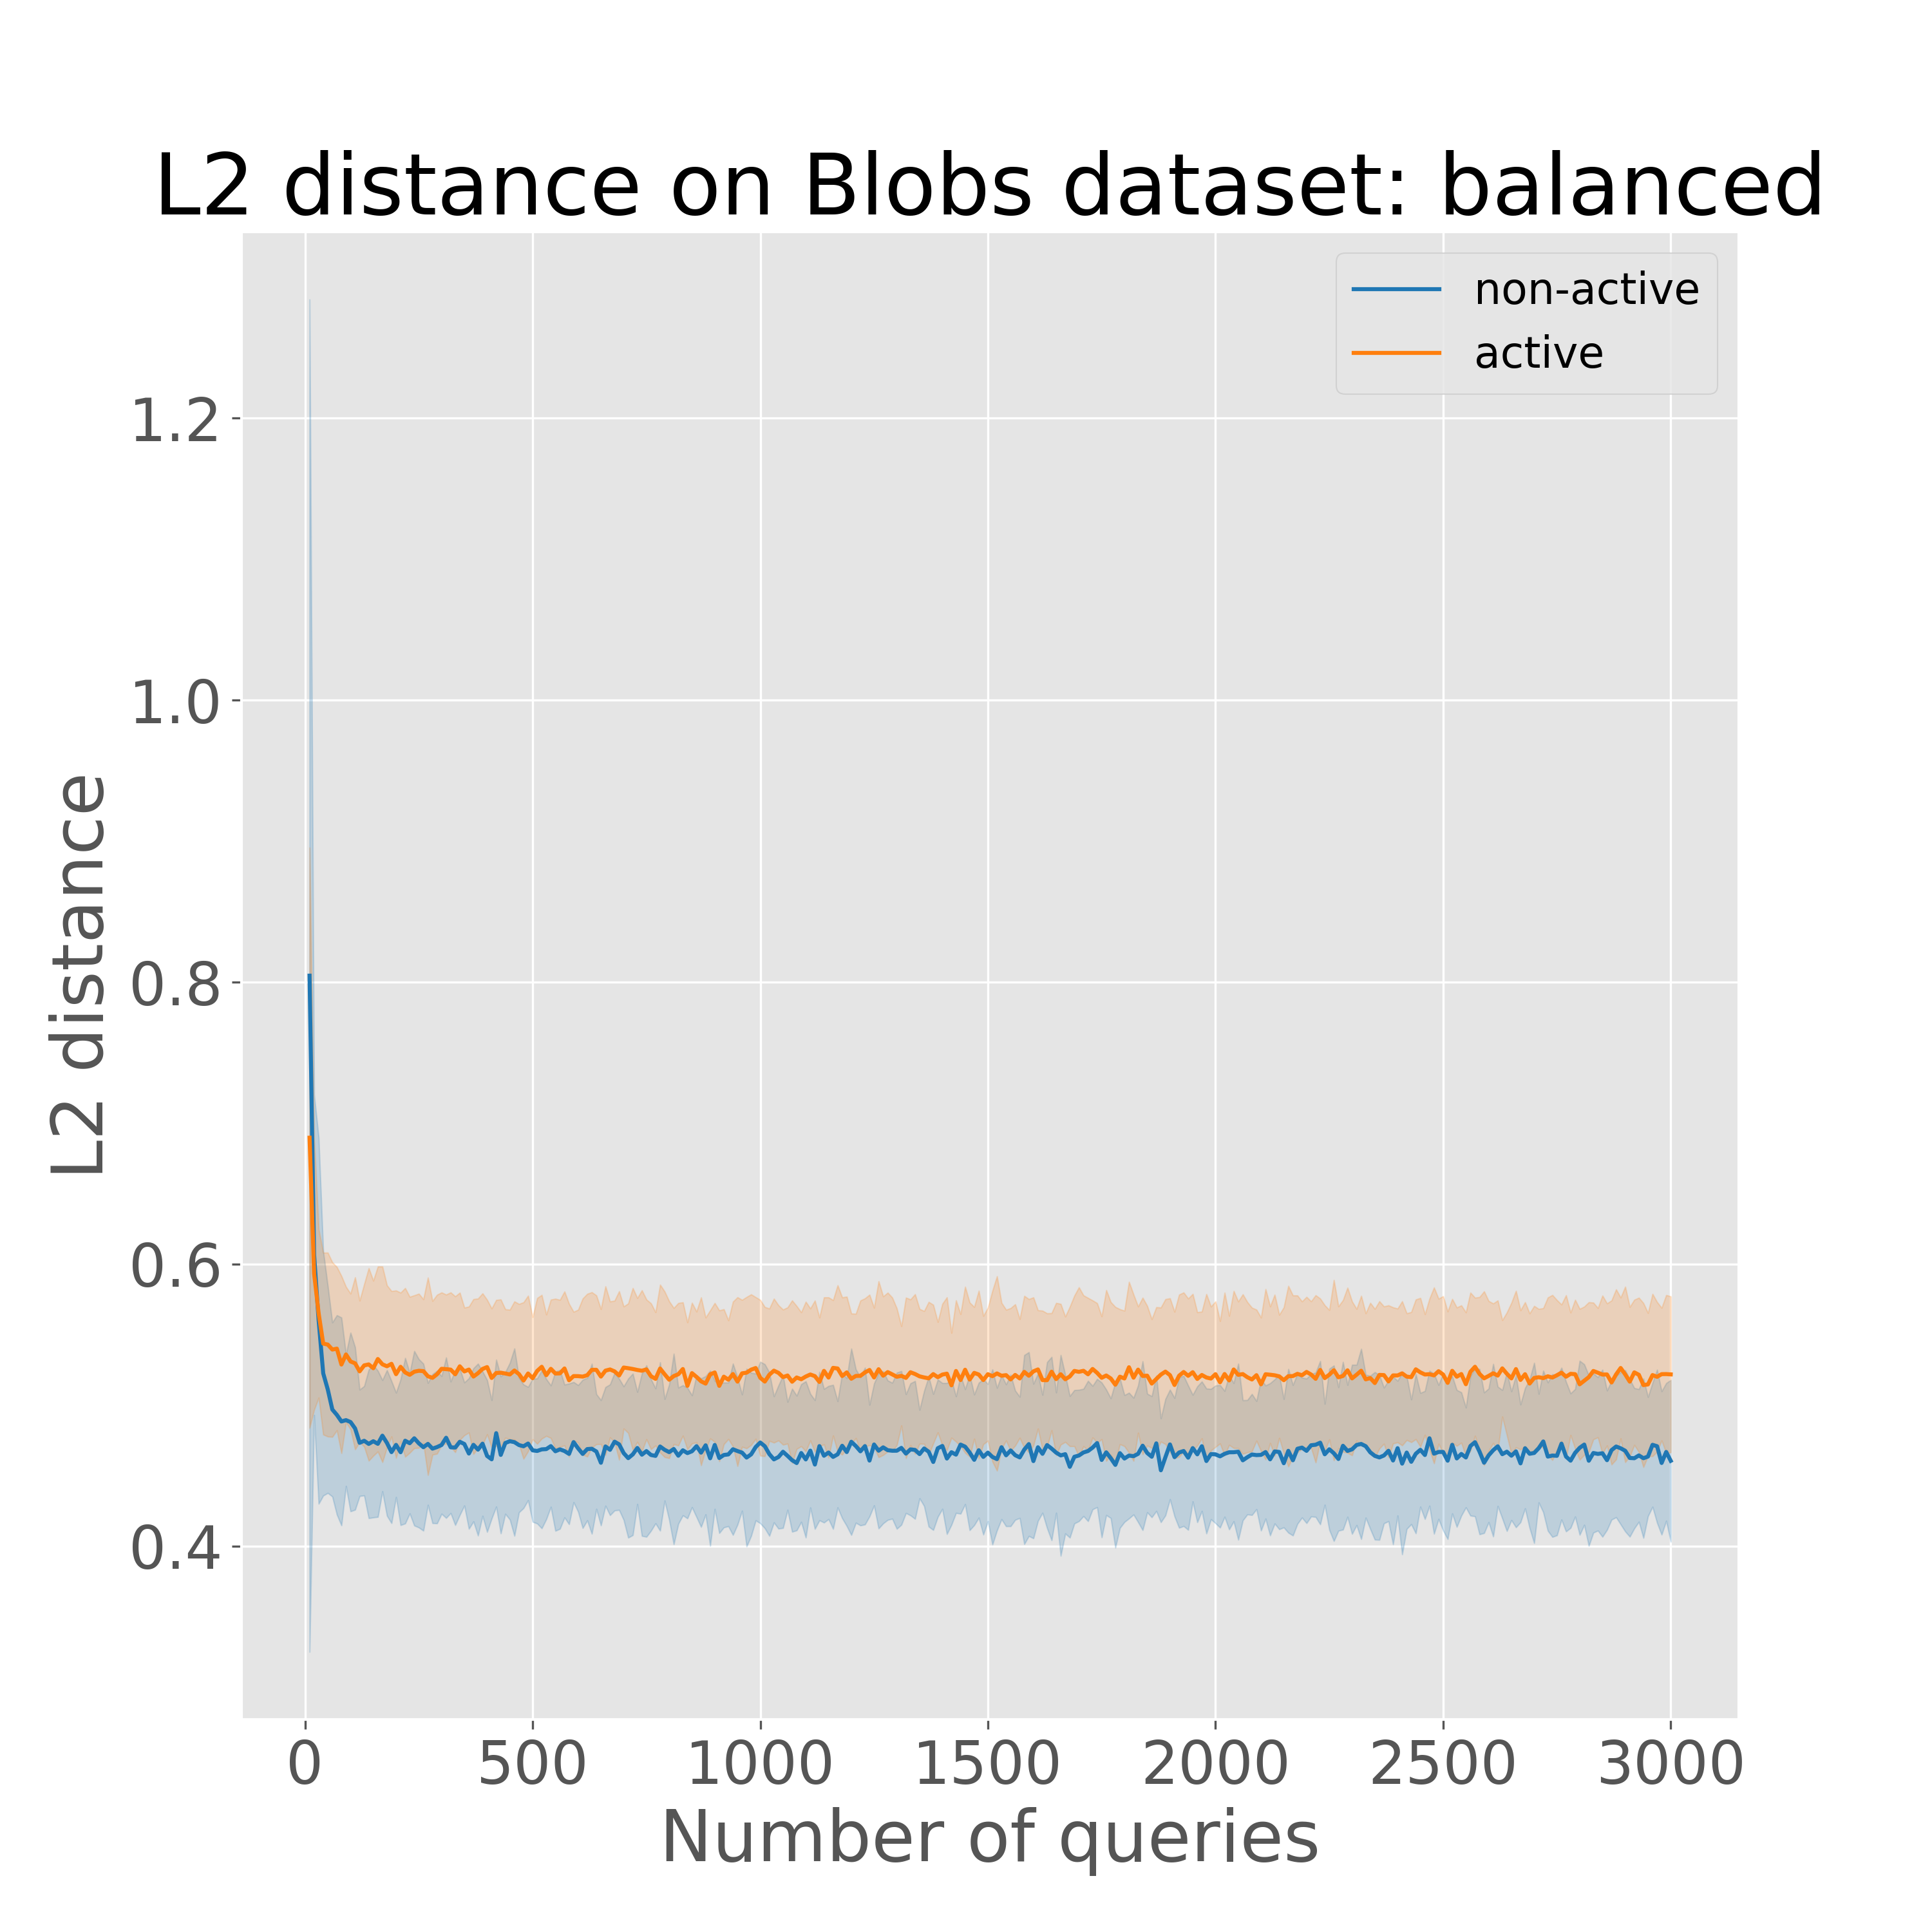
\includegraphics[width=\linewidth]{active-vs-base-blobs-l2-loss_balanced-ci}
    \caption{Balanced dataset}\label{fig:linucb-blobs-l2-loss-balanced}
  \end{minipage}%
  \begin{minipage}{.45\textwidth}
    \centering
    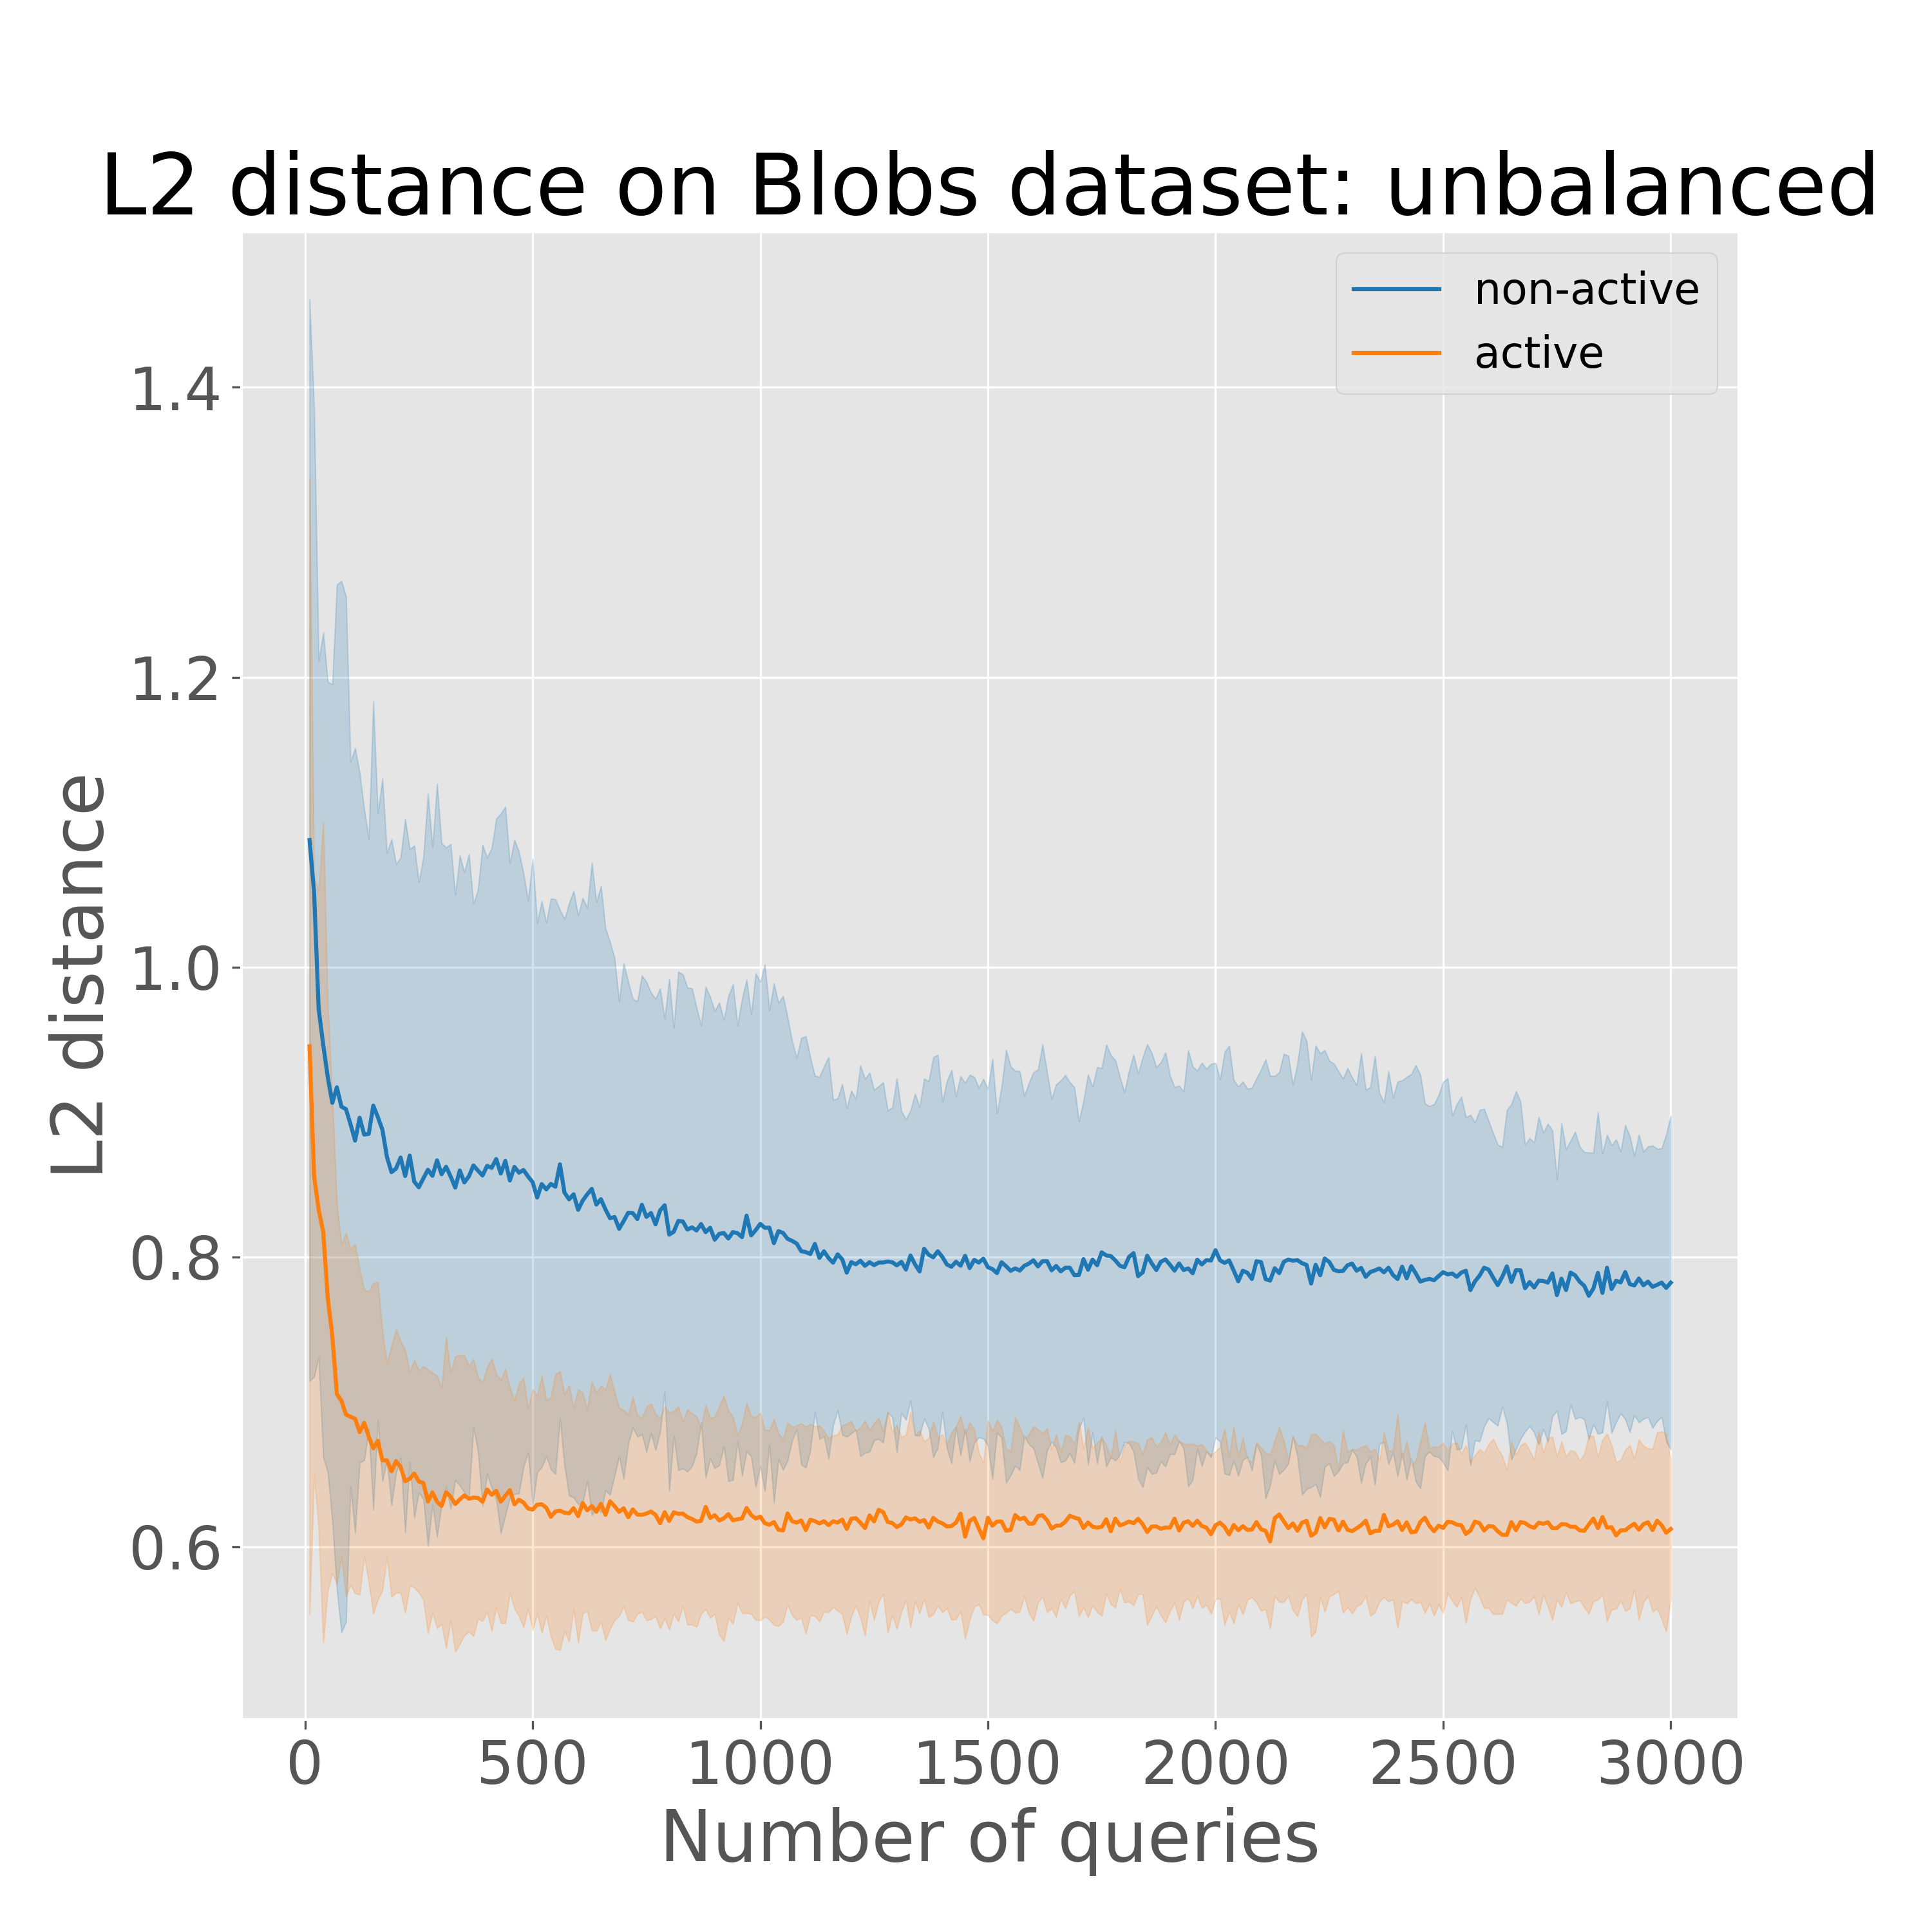
\includegraphics[width=\linewidth]{active-vs-base-blobs-l2-loss_unbalanced-ci}
    \caption{Unbalanced dataset}\label{fig:linucb-blobs-l2-loss-unbalanced}
  \end{minipage}
\end{figure}

We observe that the performance of our active algorithm is slightly worse than the baseline in the balanced data regime
but it is significantly better when we have unbalanced data. More importantly, we see that it is able to mantain low variance
in an unbalanced regime while the non-active approach doesn't enjoy this property.

\subsubsection{Experiment 2: Regret of active similarity with regime shifts}
To show that our approach leads to enhanced robustness we assume that we find ourselves in a situation
where there might be regime shifts in the data in the sense that the underlying distribution at which the similar points are provided
to the algorithm changes.

In particular, in the situation below we assume that initially the data is provided to us where there is an equal chance of getting a point
from the left blob and right blob but there at every time-step there is a $1/3000$ chance that
we will have a regime shift where the data is now sampled such that $p = 0.1$.
Plots (\ref{fig:linucb-blobs-regret-no-regime-change}) and (\ref{fig:linucb-blobs-regret-regime-change}) indicate the mean regret of the algorithm at the end
and the error bars depict the the $2.5$ and $97.5$ quantiles observed from 30 runs.

\begin{figure}[!h]
  \centering
  \begin{minipage}{.45\textwidth}
    \centering
    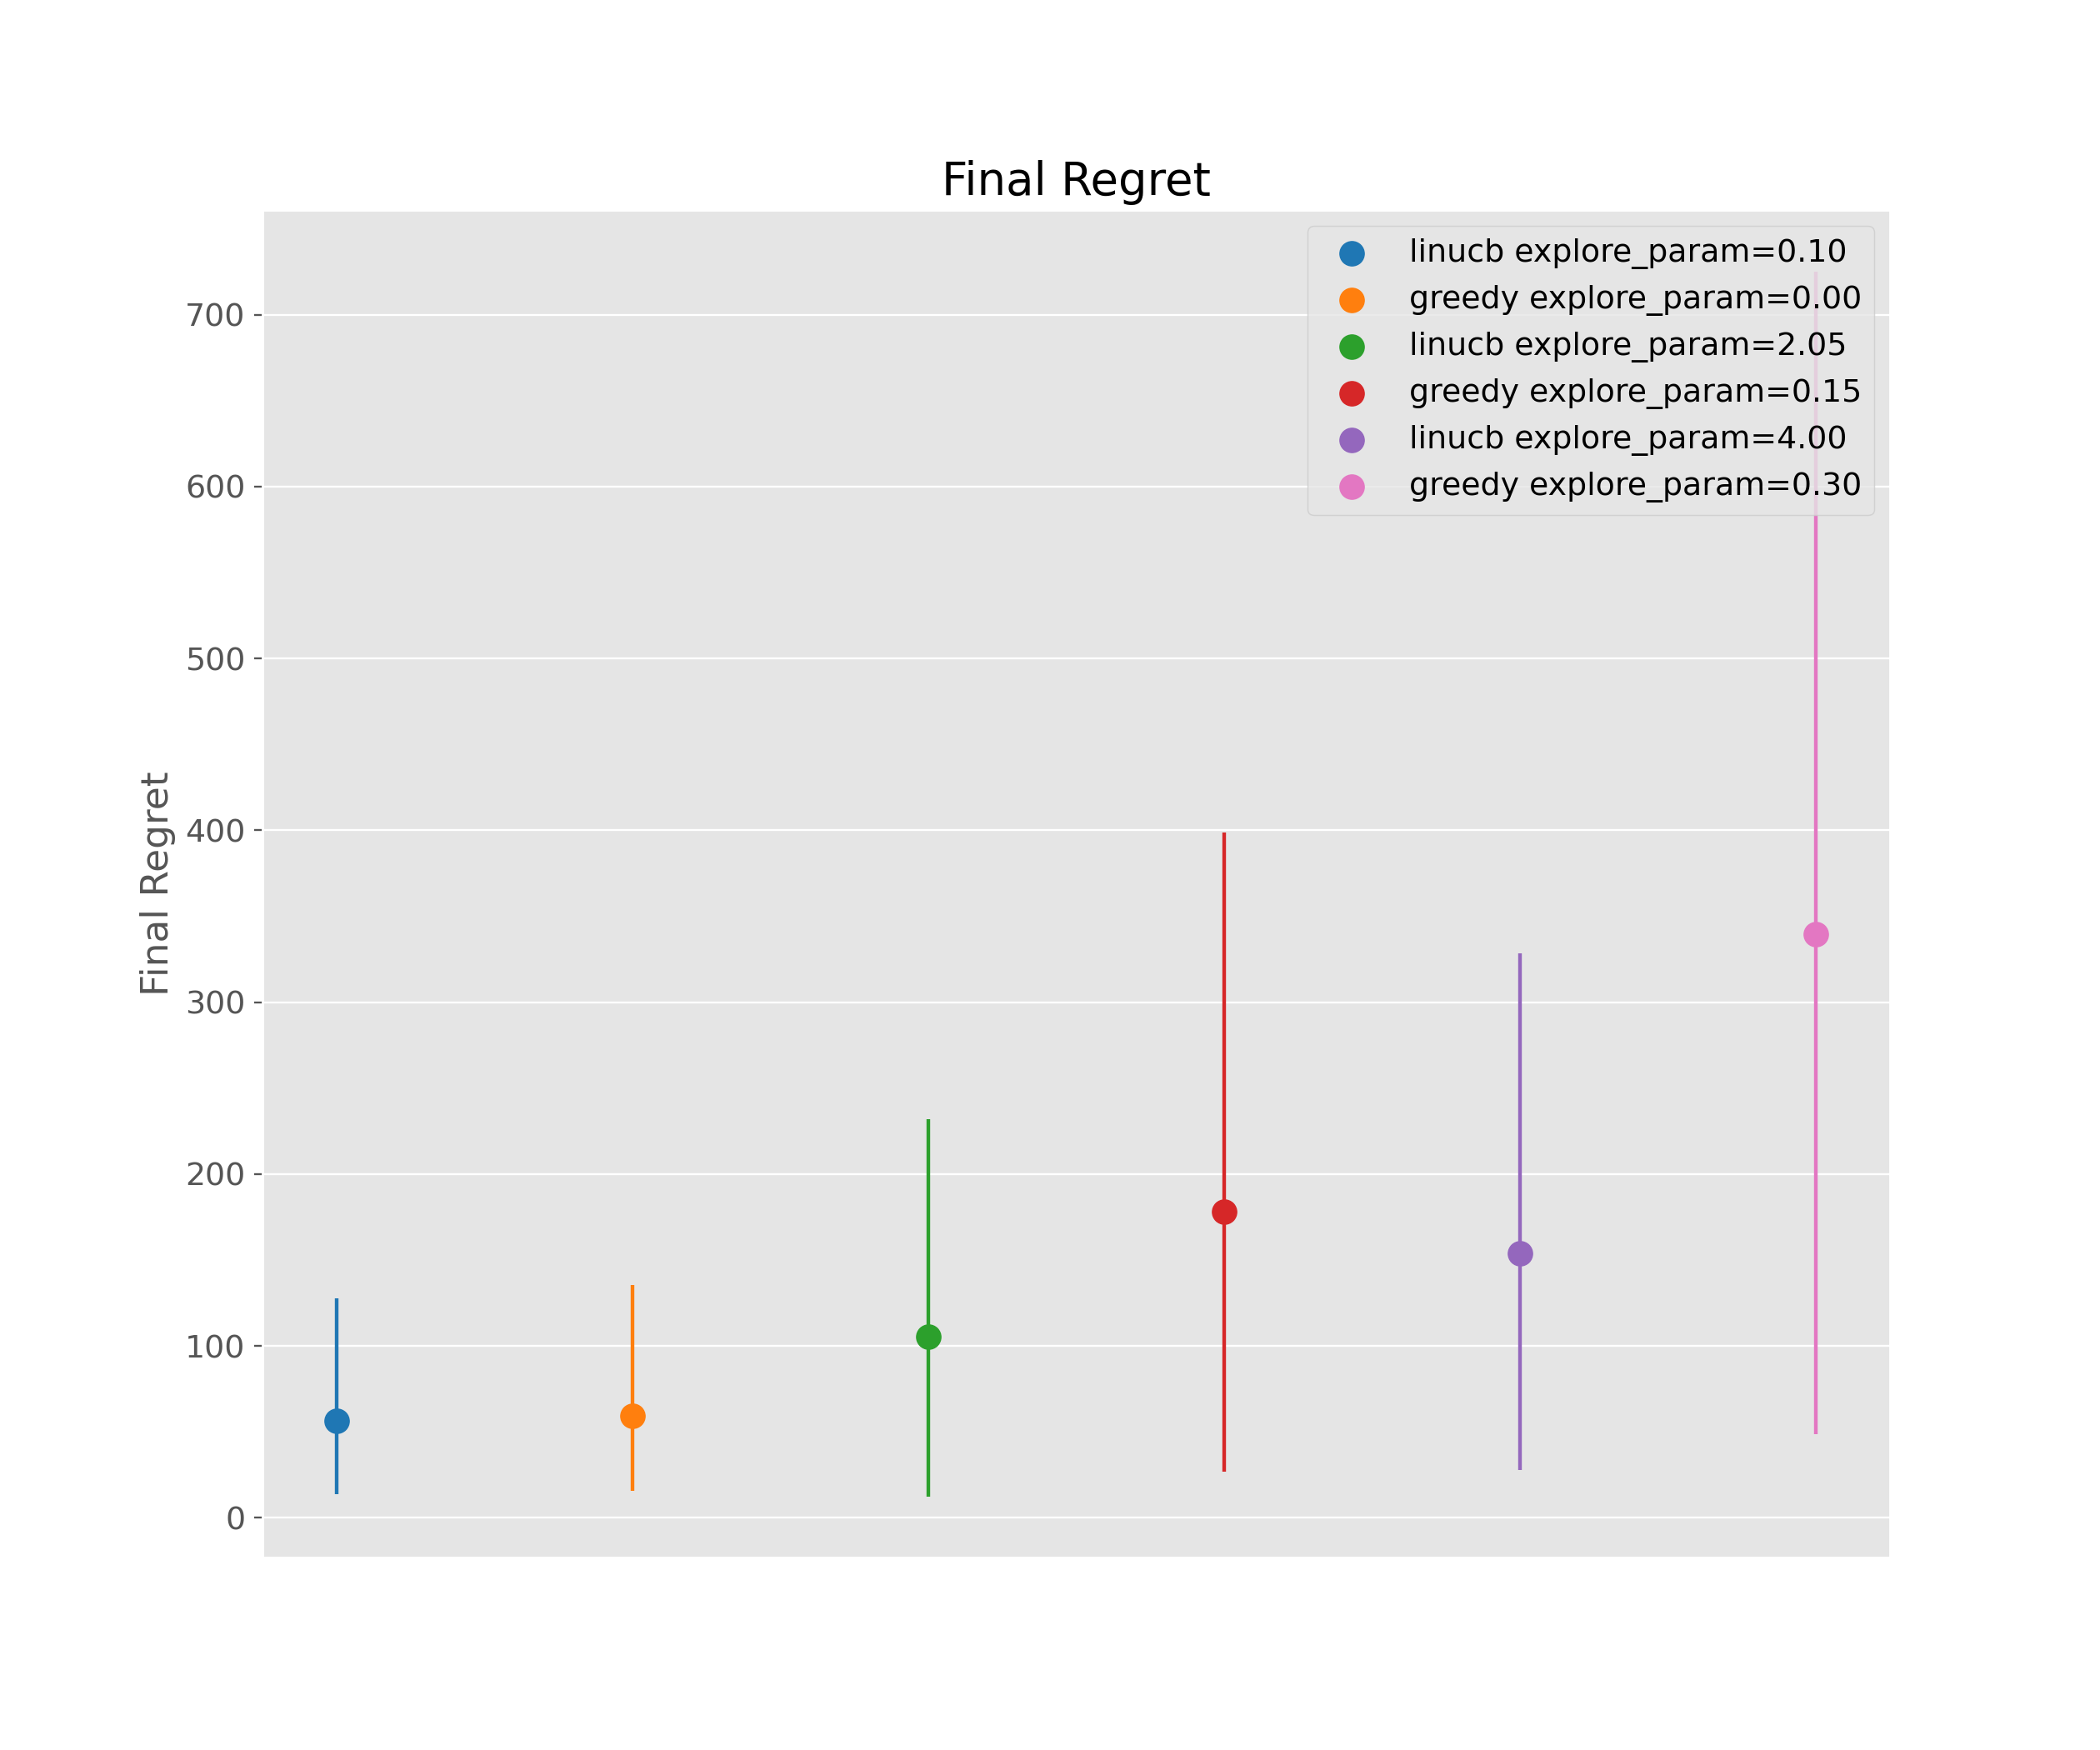
\includegraphics[width=\linewidth]{epsilon_vs_linucb_blobs}
    \caption{Regret without regime change}\label{fig:linucb-blobs-regret-no-regime-change}
  \end{minipage}%g
  \begin{minipage}{.45\textwidth}
    \centering
    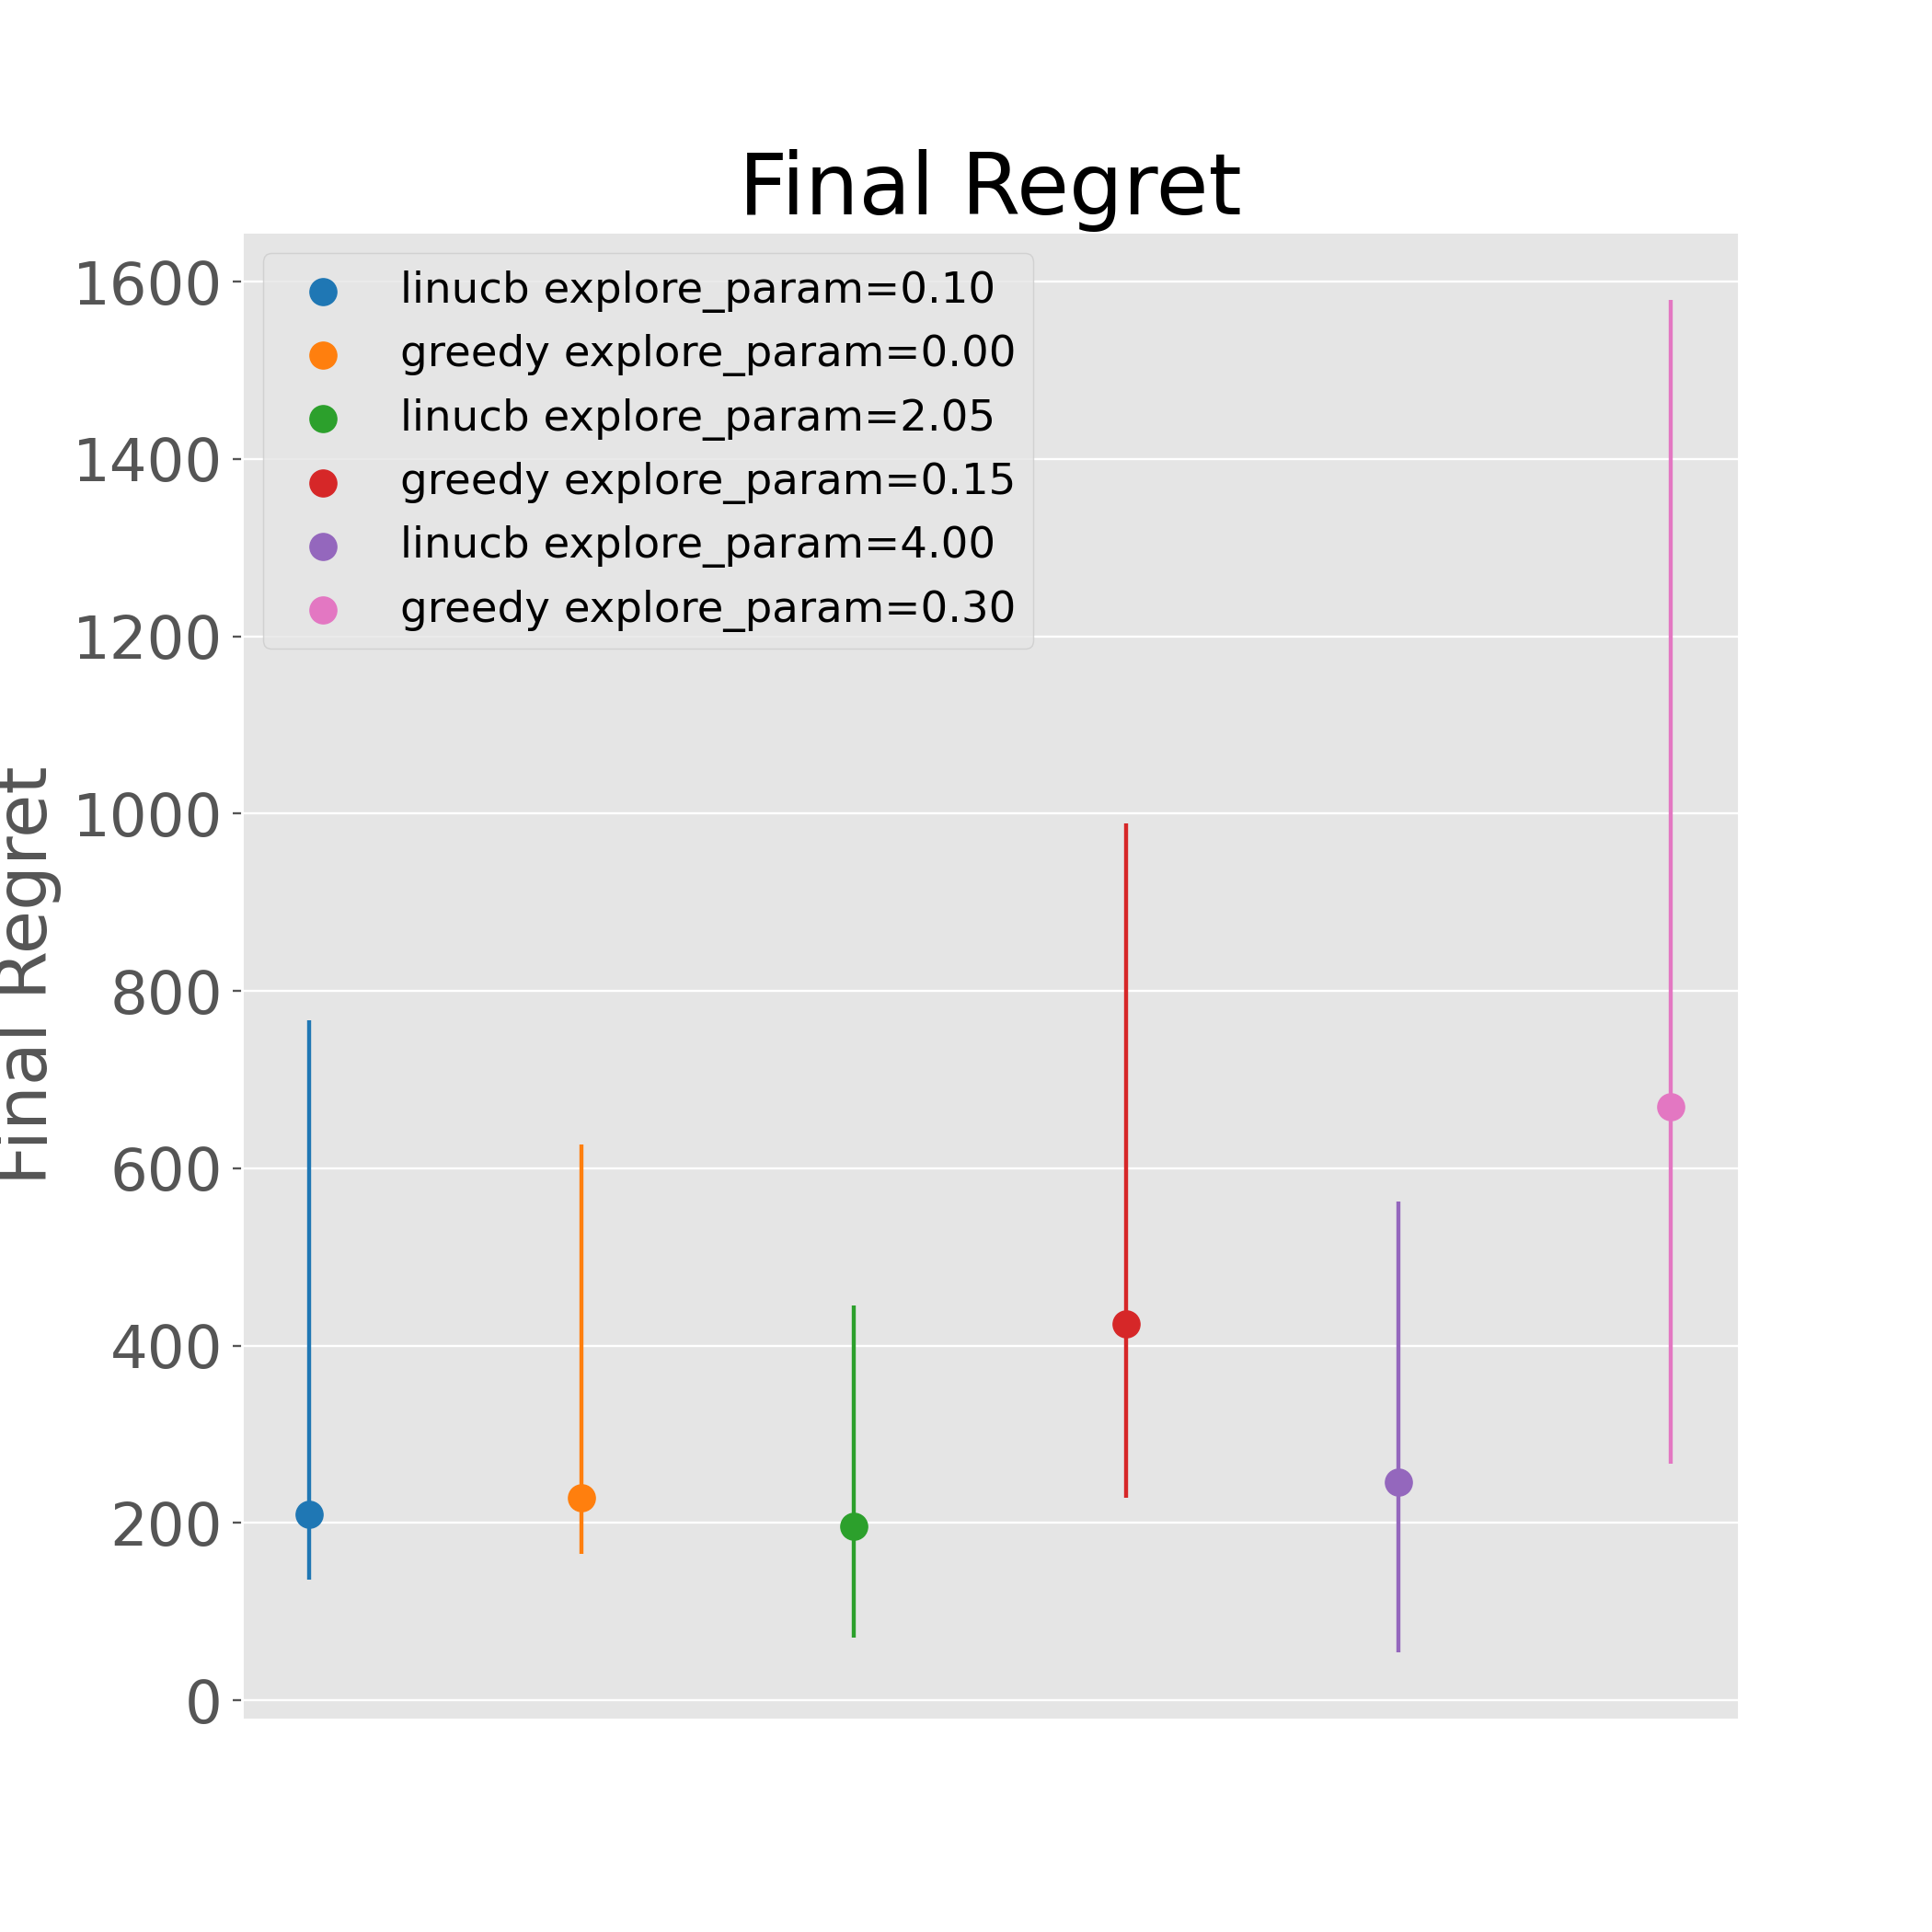
\includegraphics[width=\linewidth]{epsilon_vs_linucb_blobs_regime_change}
    \caption{Regret with regime change}\label{fig:linucb-blobs-regret-regime-change}
  \end{minipage}
\end{figure}

When there is no regime change we see that a purely greedy approach has a similar performance to an active approach with exploration parameter
of $0.1$.
However, when we allow for regime changes we see that a linucb based approach with exploration parameter $2.05$ beats all greedy algorithms,
not only in terms of a lower mean regret but also in terms of a significantly lower $97.5$ quantile and lower $2.5$ quantile.

\section{Discussion of results}
The results of the experiments show a mixed picture.
On the one hand the results for Active-LinUCB and OnSim-LinUCB show the benefits that our approach has
compared to a naive use of the data or over an epsilon greedy baseline.
This is reasonable as the matrix used in the algorithm naturally favors a diversity of points which allows
the algorithm to explore the two blobs more efficiently.

However, we observe that for our neural algorithms, the performance varies significantly depending on the particular optimization
strategy used and whether we use normalized or non-normalized features.
This situation is aggravated further by the $O(p^2)$ memory requirements (due to the matrix computation) of the algorithm and the $O(Tp^2)$ time complexity requirements (due to the computation of the optimism).
All of the above suggests that even if there is an advantage, the algorithms are not feasible for practical settings.

Finally, it is important to note that even if the linear approach works, the reason why it performs so well is because it implicitely uses
some notion of diversity with regards to the the eucledean space.
This is limiting and contradictory in that precisely such a notion is what we are trying to learn.

An interesting alternative which would solve the aformentioned issues realted to the complexity of the algorithms and
the issues pertaining to the notion of space in the linear case is to use only a shallow notion of UCB as proposed in \cite{shallow} or
\cite{deep-bayesian-bandits-show-down}.
This way we can avoid the expensive matrix computations and optimize based on a diversity of vectors with respect to the current embedding
used by the neural network, which is constantly changing.

\section{Conclusion and Future Work}
In this work we studied a variety of approaches to solving the active learning and online versions of similarity learning using UCB based appraches.
Although our work suggests that the methods proposed are not enough for practical use, we believe that the tests conducted suggests that there is
value in exploring these approaches, especially in situations where there might be shifts in the underlying distribution of the data and the
amount of similar pairs that we get.
As a future direction forward we propose to work with shallow methods of exploration to avoid expensive matrix computations while
retaining the flexibility of neural based appraches.

\bibliography{refs}
\bibliographystyle{plain}

\newpage
\appendix
\section{Appendix}

\subsection{Algorithms omitted from main text}

\begin{algorithm}
  \setstretch{1.2}
    \SetKwInOut{Input}{Input}
    \Input{$\epsilon$ learning rate, $E$ number of epochs, dataset $\{(x_i^{k_i}, y_i^{k_i}, r_i)\}_{i=1}^t$, $b_s$ batch size}

    optimizer $\gets$ SGD($\epsilon, \theta$)\;
    \For{$j = 1, \dots, E$}{
      $\mathcal{D} \gets \{(x_1^{k_1}, y_1^{k_1}, r_1), \dots, (x_t^{k_t}, y_t^{k_t}, r_t)$ \;
      \While{$\mathcal{D}$ is not empty}{
        Sample minibatch $M$ of size $b_s$ from the training examples\;
        $l = \frac{1}{M}\sum_{(x_i^{k_{i}}, y_i^{k_i}, r_i) \in M} (\phi(x_i^{k_{i}}, y_i^{k_i}) - r_i)^2$\;
        $\theta \gets$ update using optimizer with loss $l$\;

        Remove $M$ from $\mathcal{D}$\;
      }
    }
    \caption{Train}\label{algo:train}
  \end{algorithm}


  \begin{algorithm}
  \setstretch{1.2}
    \SetKwInOut{Input}{Input}
    \Input{Rounds $T$ and exploration parameter $\alpha$}
    $A \gets I_{n^2}$\;
    $b \gets 0_{n^2}$\;
    \For{$t \in [T]$}{
      $\theta_t \gets A^{-1}b$
      Observe $K$ pairs of vectors $x^k \in \mathbb{R}^n$, $y^k \in \mathbb{R}^n$\;
      Create $z_{t,k} = (x_1^k, y_1^k, x_1^k, y_1^k, \dots, x_n^k y_{n-1}^k, x_n^k ,y_n^k)$\;
      \For{$k \in [K]$}{
        $p_{t,a} \gets \theta_t^\top z_{t,k} + \alpha \sqrt{z_{t,k}^\top A^{-1} z_{t,a}}$
      }
      Choose action $k_t = \text{argmax}_a p_{t,a}$ with ties broken arbitrarily\;
      Observe payoff $ r_t \in \{-1,1 \}$\;
      $A \gets A + z_{t,k_t}z_{t,k_t}^\top$\;
      $b \gets z_{t,k_t}r_t$\;
    }
    \caption{OnSim-LinUCB}\label{algo:onsim-linucb}
\end{algorithm}



\begin{algorithm}
  \setstretch{1.2}
    \SetKwInOut{Input}{Input}
    \Input{Queries $T$, exploration parameter $\alpha$, $\tau_r$ frequency of resets, $\tau_T$ frequency of training, $E$ epochs for training, $b_s$ batch size for training, $\epsilon$ learning rate.}
    $A \gets I_{p}$\;
    \For{$t \in [T]$}{
      Sample $K$ pairs of vectors $x_t^k \in \mathbb{R}^n$, $y_t^k \in \mathbb{R}^n$ from dataset $D$\;
      \For{$k \in [K]$}{
        $p_{t,k} \gets \alpha \sqrt{(\nabla_\theta \phi(x_t^k, y_t^k))^\top A^{-1}\nabla_\theta\phi(x_t^k,y_t^k)}$\;
        \label{change:active-neuralucb}
      }
      Choose pair $k_t = \text{argmax}_kp_{t,k}$ with ties broken arbitrarily\;
      Query label $ r_t \in \{-1,1\}$\;
      \If{$t \mod \tau_r = 0$ }{
        $\theta \gets \text{Train}(\epsilon,E, \{(x_i^{k_i}, y_i^{k_i}, r_i)\}_{i=1}^t,b_s)$\;
      }
      \If{$t \mod \tau_T = 0$ }{
        $A \gets I_p$
      }
      $A \gets A + \nabla_\theta \phi(x_t^k, y_t^k)(\nabla_\theta\phi(x_t^k,y_t^k))^\top$\;
    }
    \caption{Active-NeuralUCB}\label{algo:active-neuralucb}
  \end{algorithm}

\newpage
\subsection{MNIST dataset}
\label{sec:additional-experiments}
This section contains additional experiments we ran but omit from the main text due to
space considerations.

Our first set of experiments contains the equivalent of the experiments performed on the crescent moons dataset
but for MNIST.
Because of the size of the dataset, we were not able to run the experiment on the full dataset and instead
first performed PCA on it and reduced it to 15 dimensional space.
As can be seen for the figures the results are significantly less promising than the ones on the crescent moons dataset.
We attribute this, mostly due to the fact that the dimensionality can't capture the results adequately
All of the settings are the same as before except for the fact that we run the experiment with more queries or though a longer time-span.

Figures \ref{fig:svm-non-normalized-ci-mnist} and \ref{fig:svm-normalized-ci-mnist} compare the performance of the learned features in the active version of the algorithm using SVMs.
Figures \ref{fig:l2-loss-normalized-ci-mnist} and \ref{fig:l2-loss-non-normalized-ci-mnist} compare the performance of the learned metric with respect to the $l_2$ loss.
Figure \ref{fig:online-epsilon-vs-neural-ci-mnist} compares the performance of an epsilon greedy vs the neural version of the algorithm in the online setting.



% add figures
\begin{figure}[h]
  \centering
  \begin{minipage}{.45\textwidth}
    \centering
    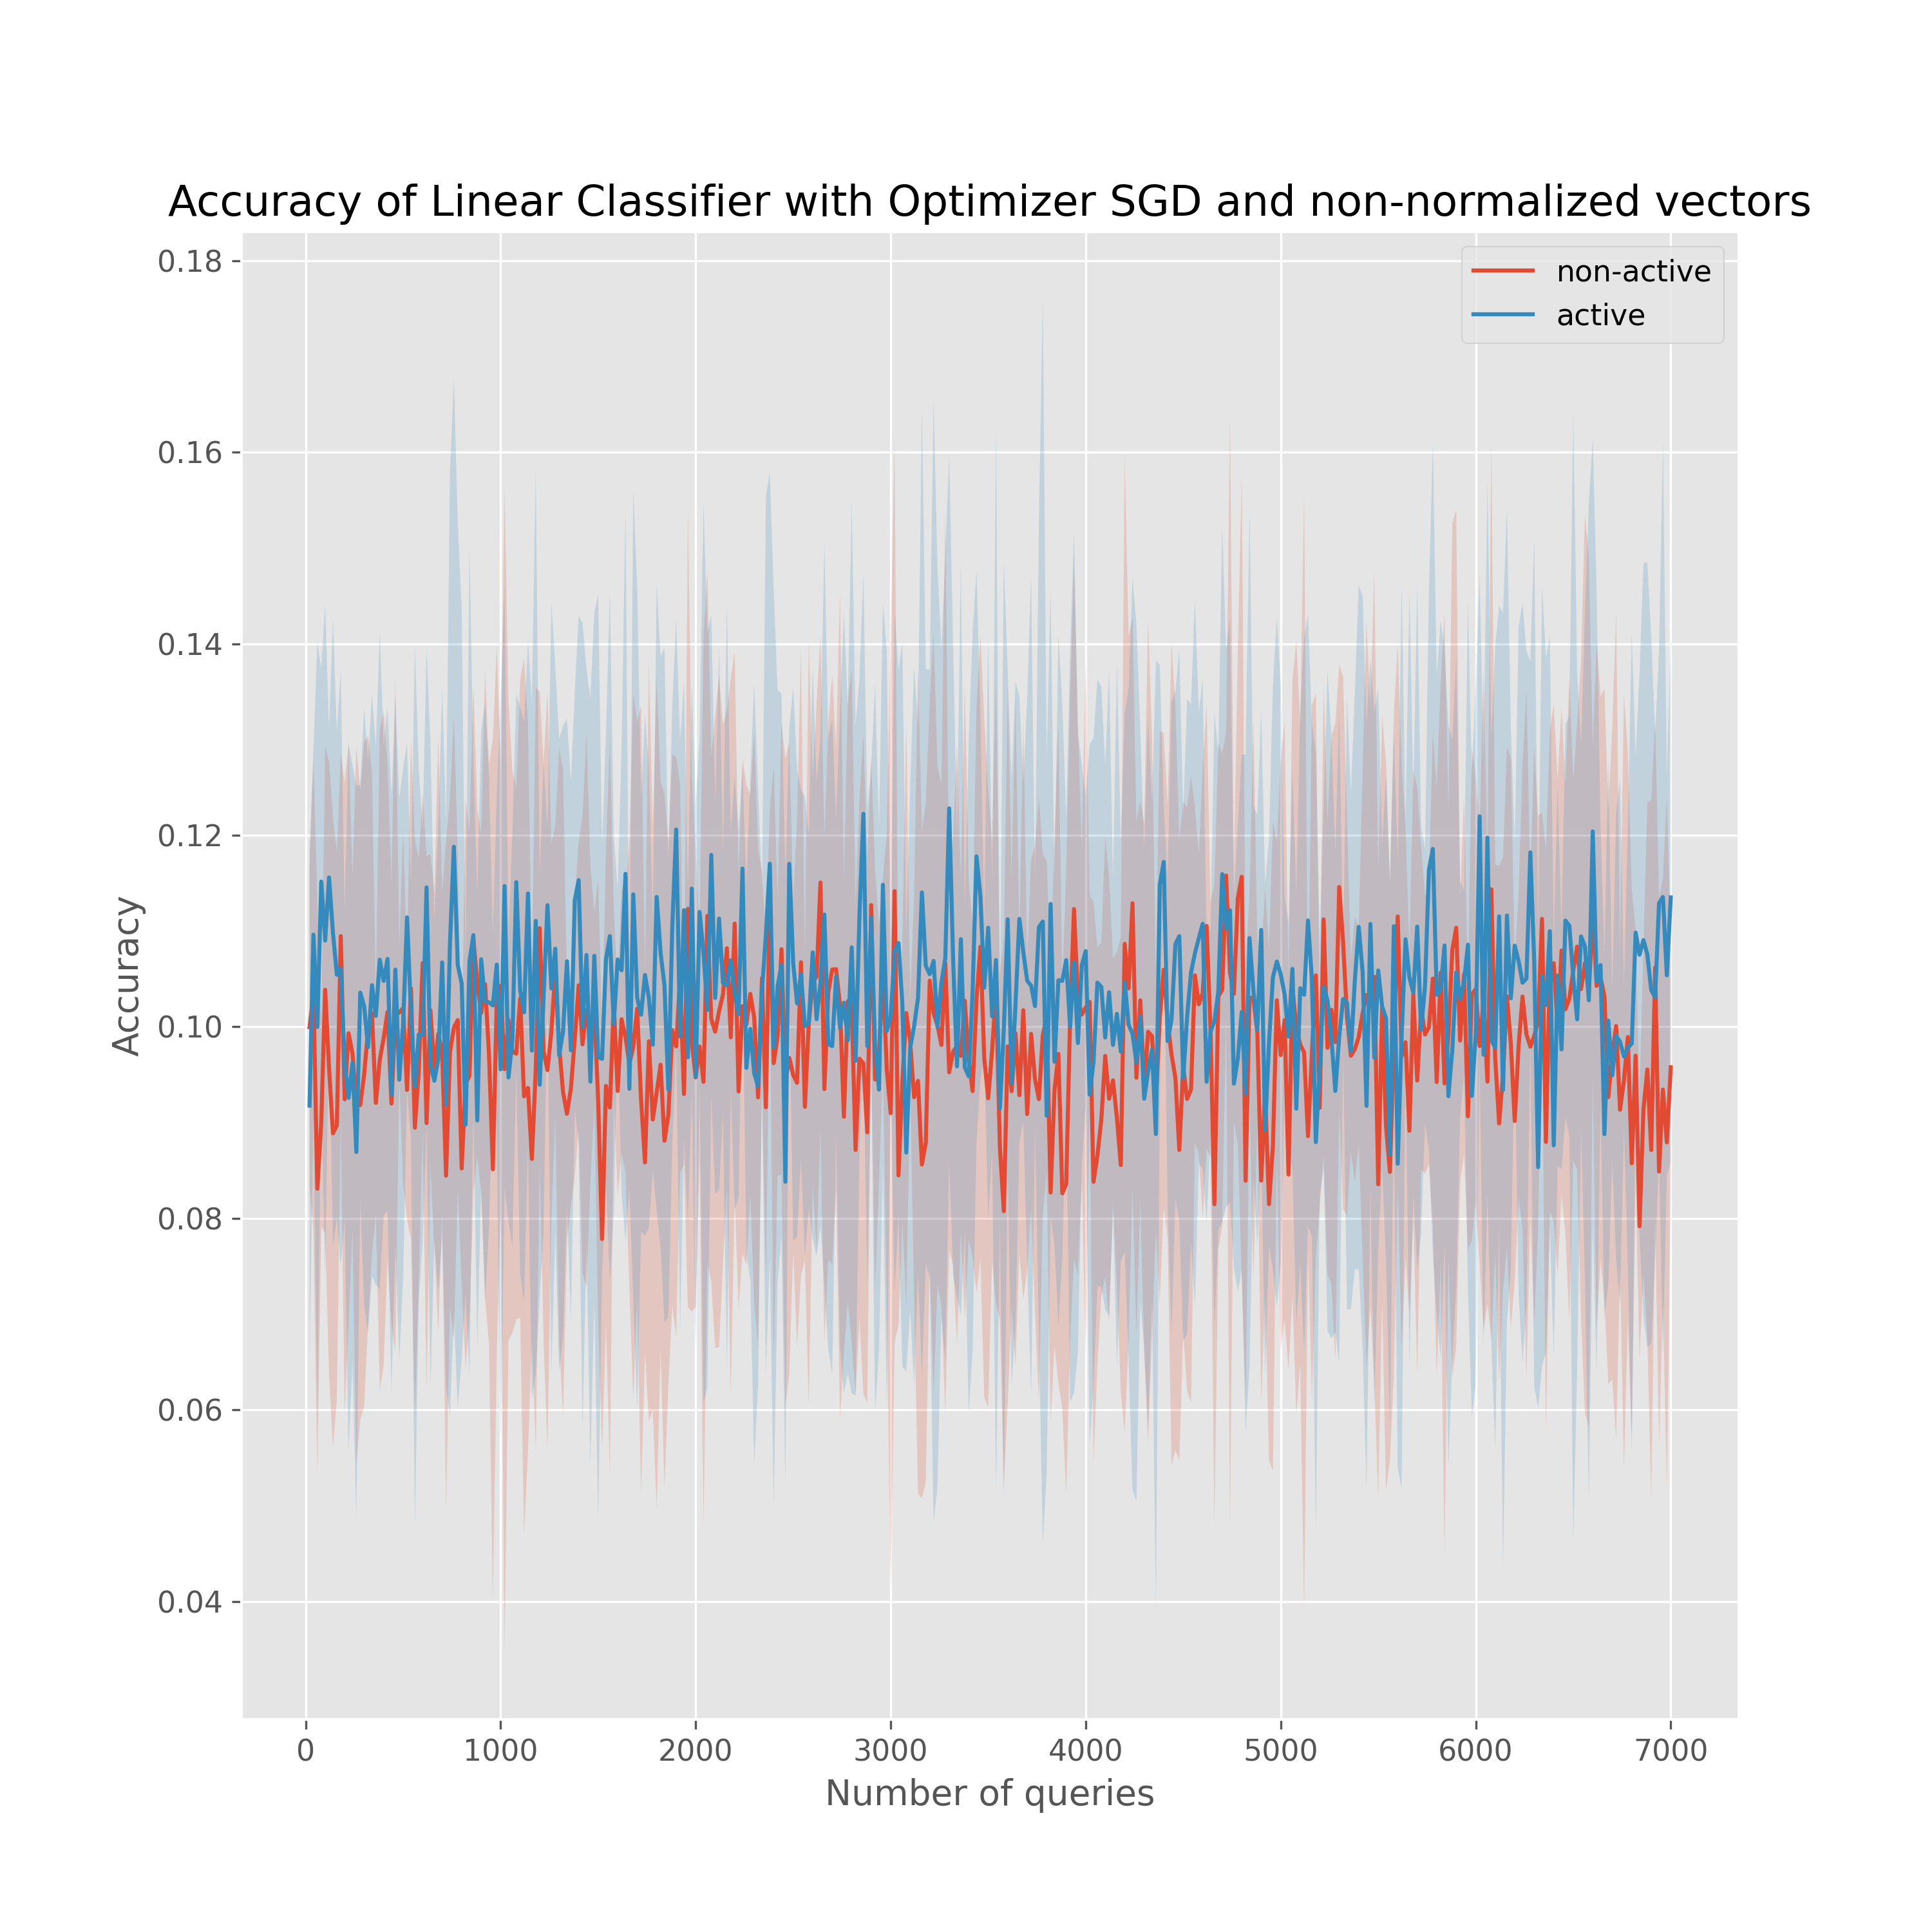
\includegraphics[width=\linewidth]{active-vs-base-mnist-linear-loss-SGD-non-normalized-ci}
  \end{minipage}%
  \begin{minipage}{.45\textwidth}
    \centering
    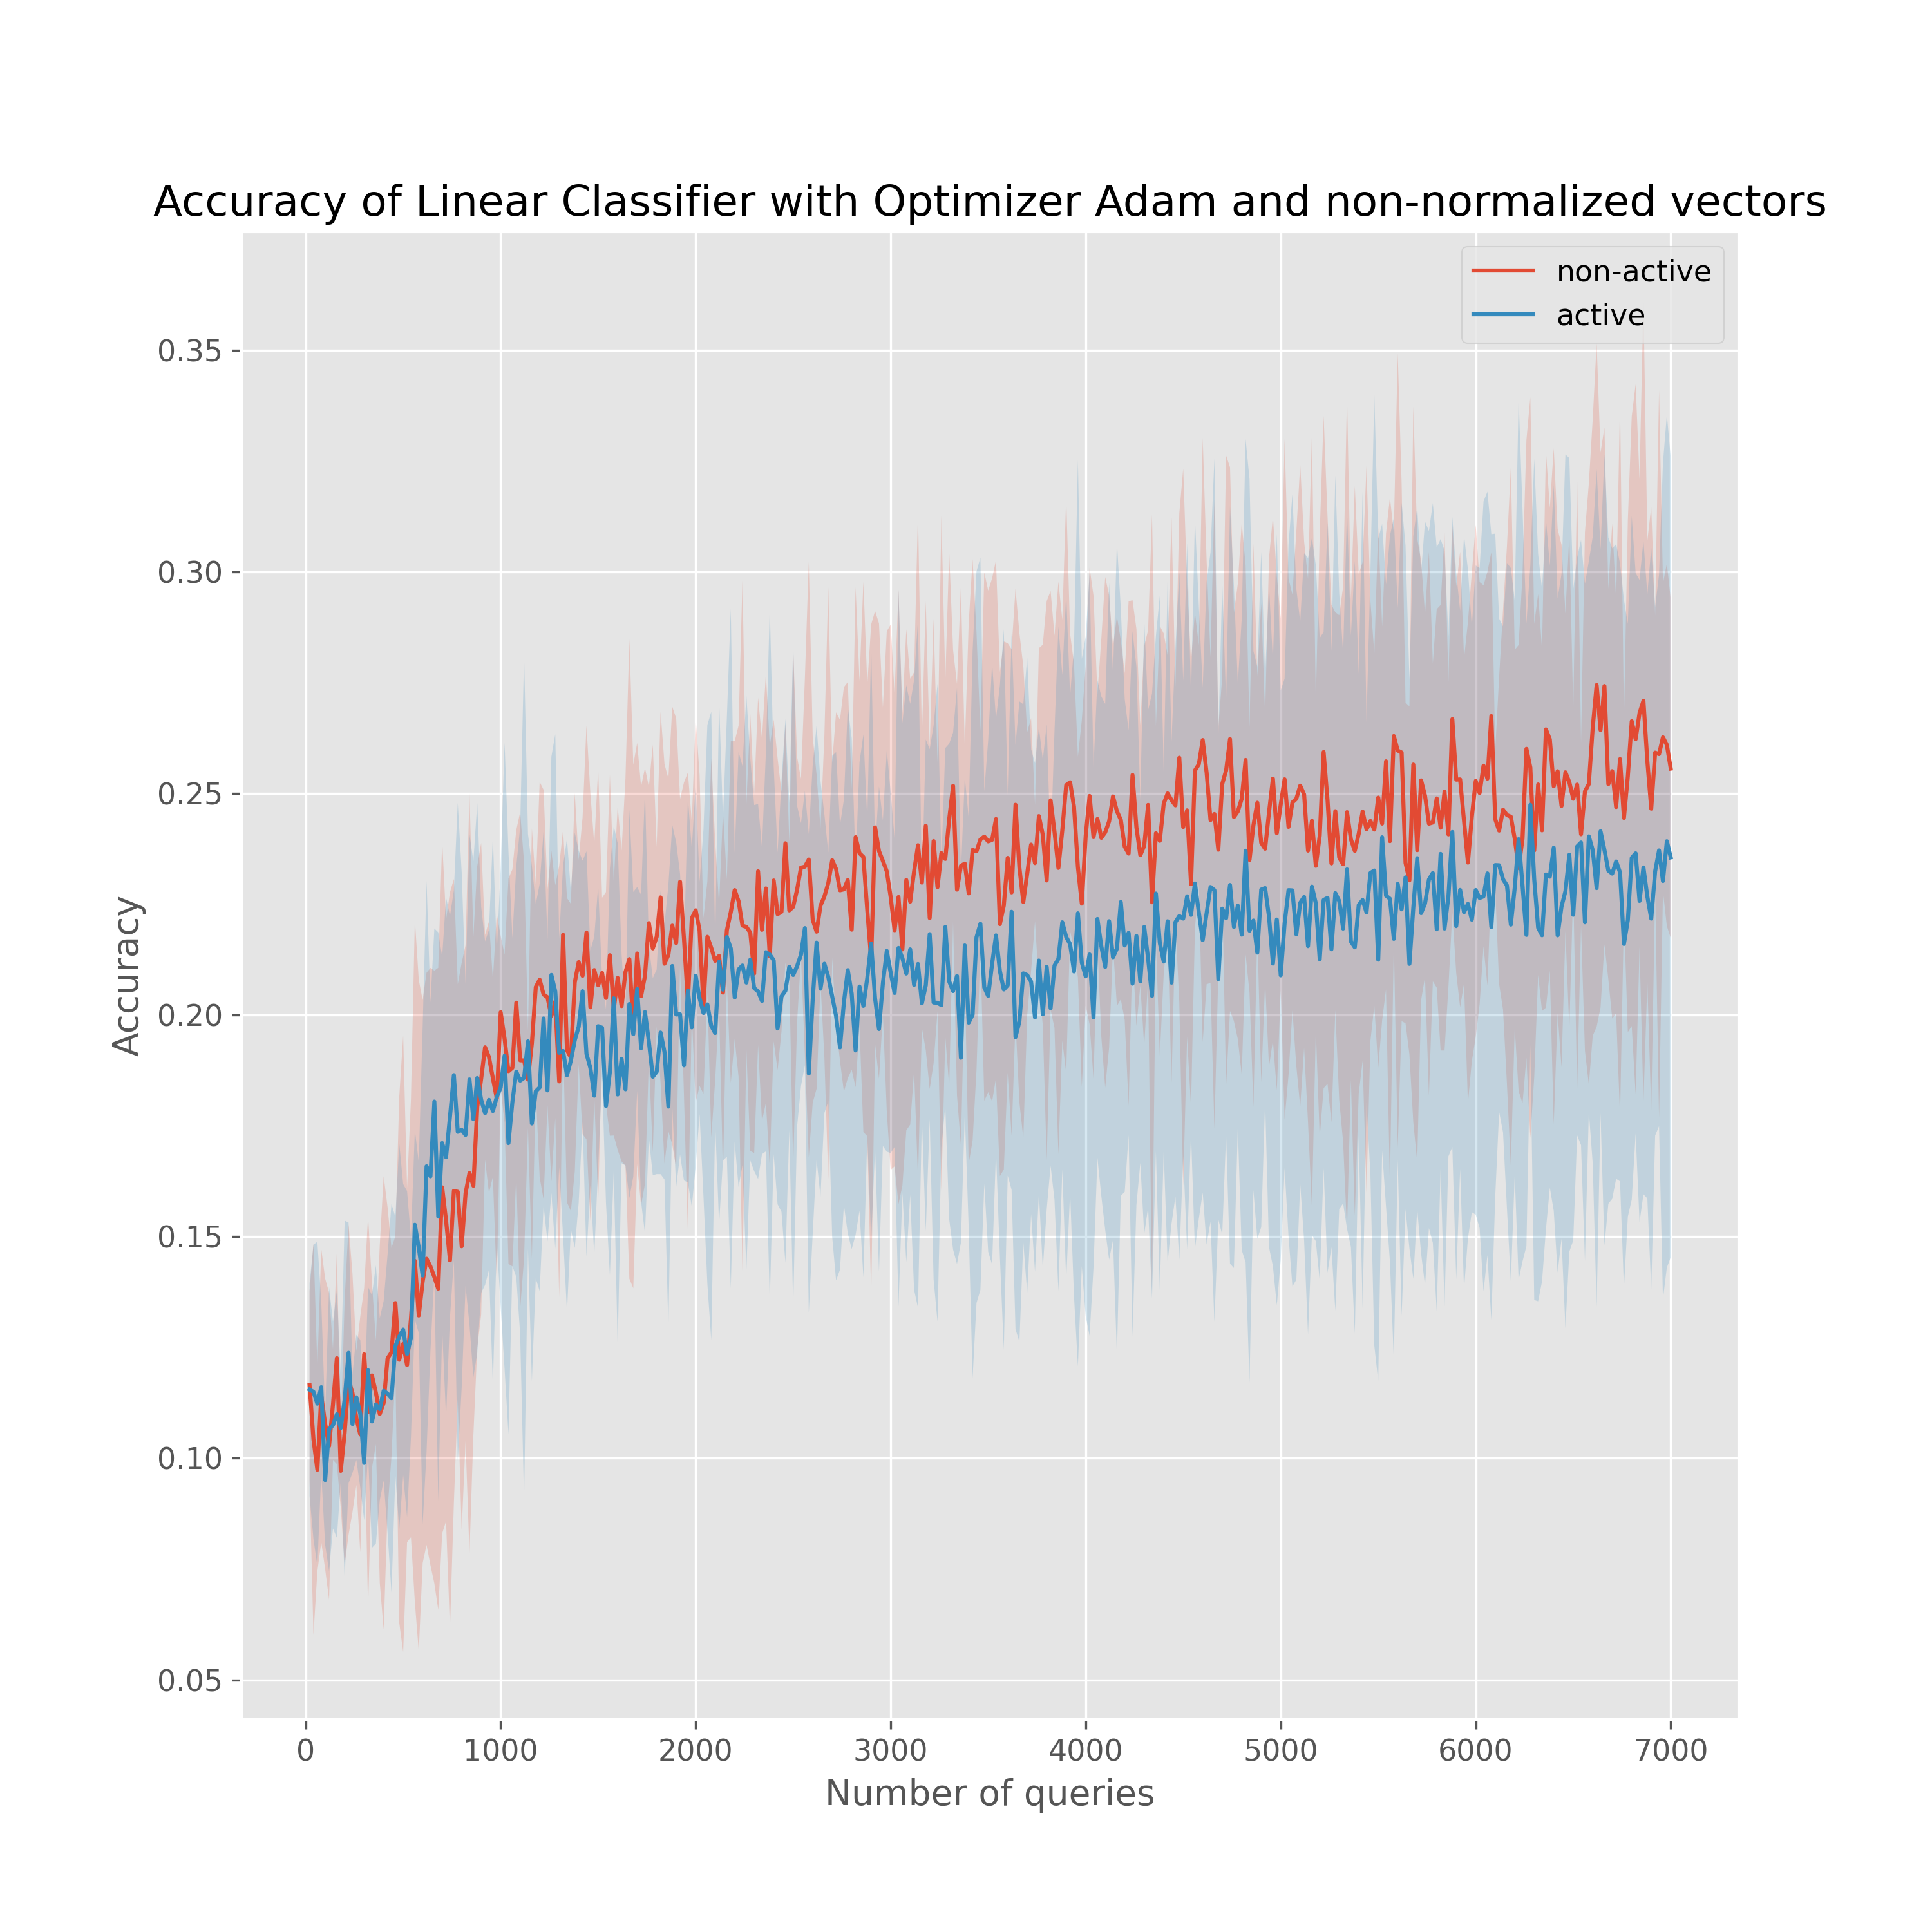
\includegraphics[width=\linewidth]{active-vs-base-mnist-linear-loss-Adam-non-normalized-ci}
  \end{minipage}
  \caption{Performance SVM on non-normalized learned features SGD (left) vs Adam (right)}\label{fig:svm-non-normalized-ci-mnist}
\end{figure}


% add figures
\begin{figure}[h]
  \centering
  \begin{minipage}{.45\textwidth}
    \centering
    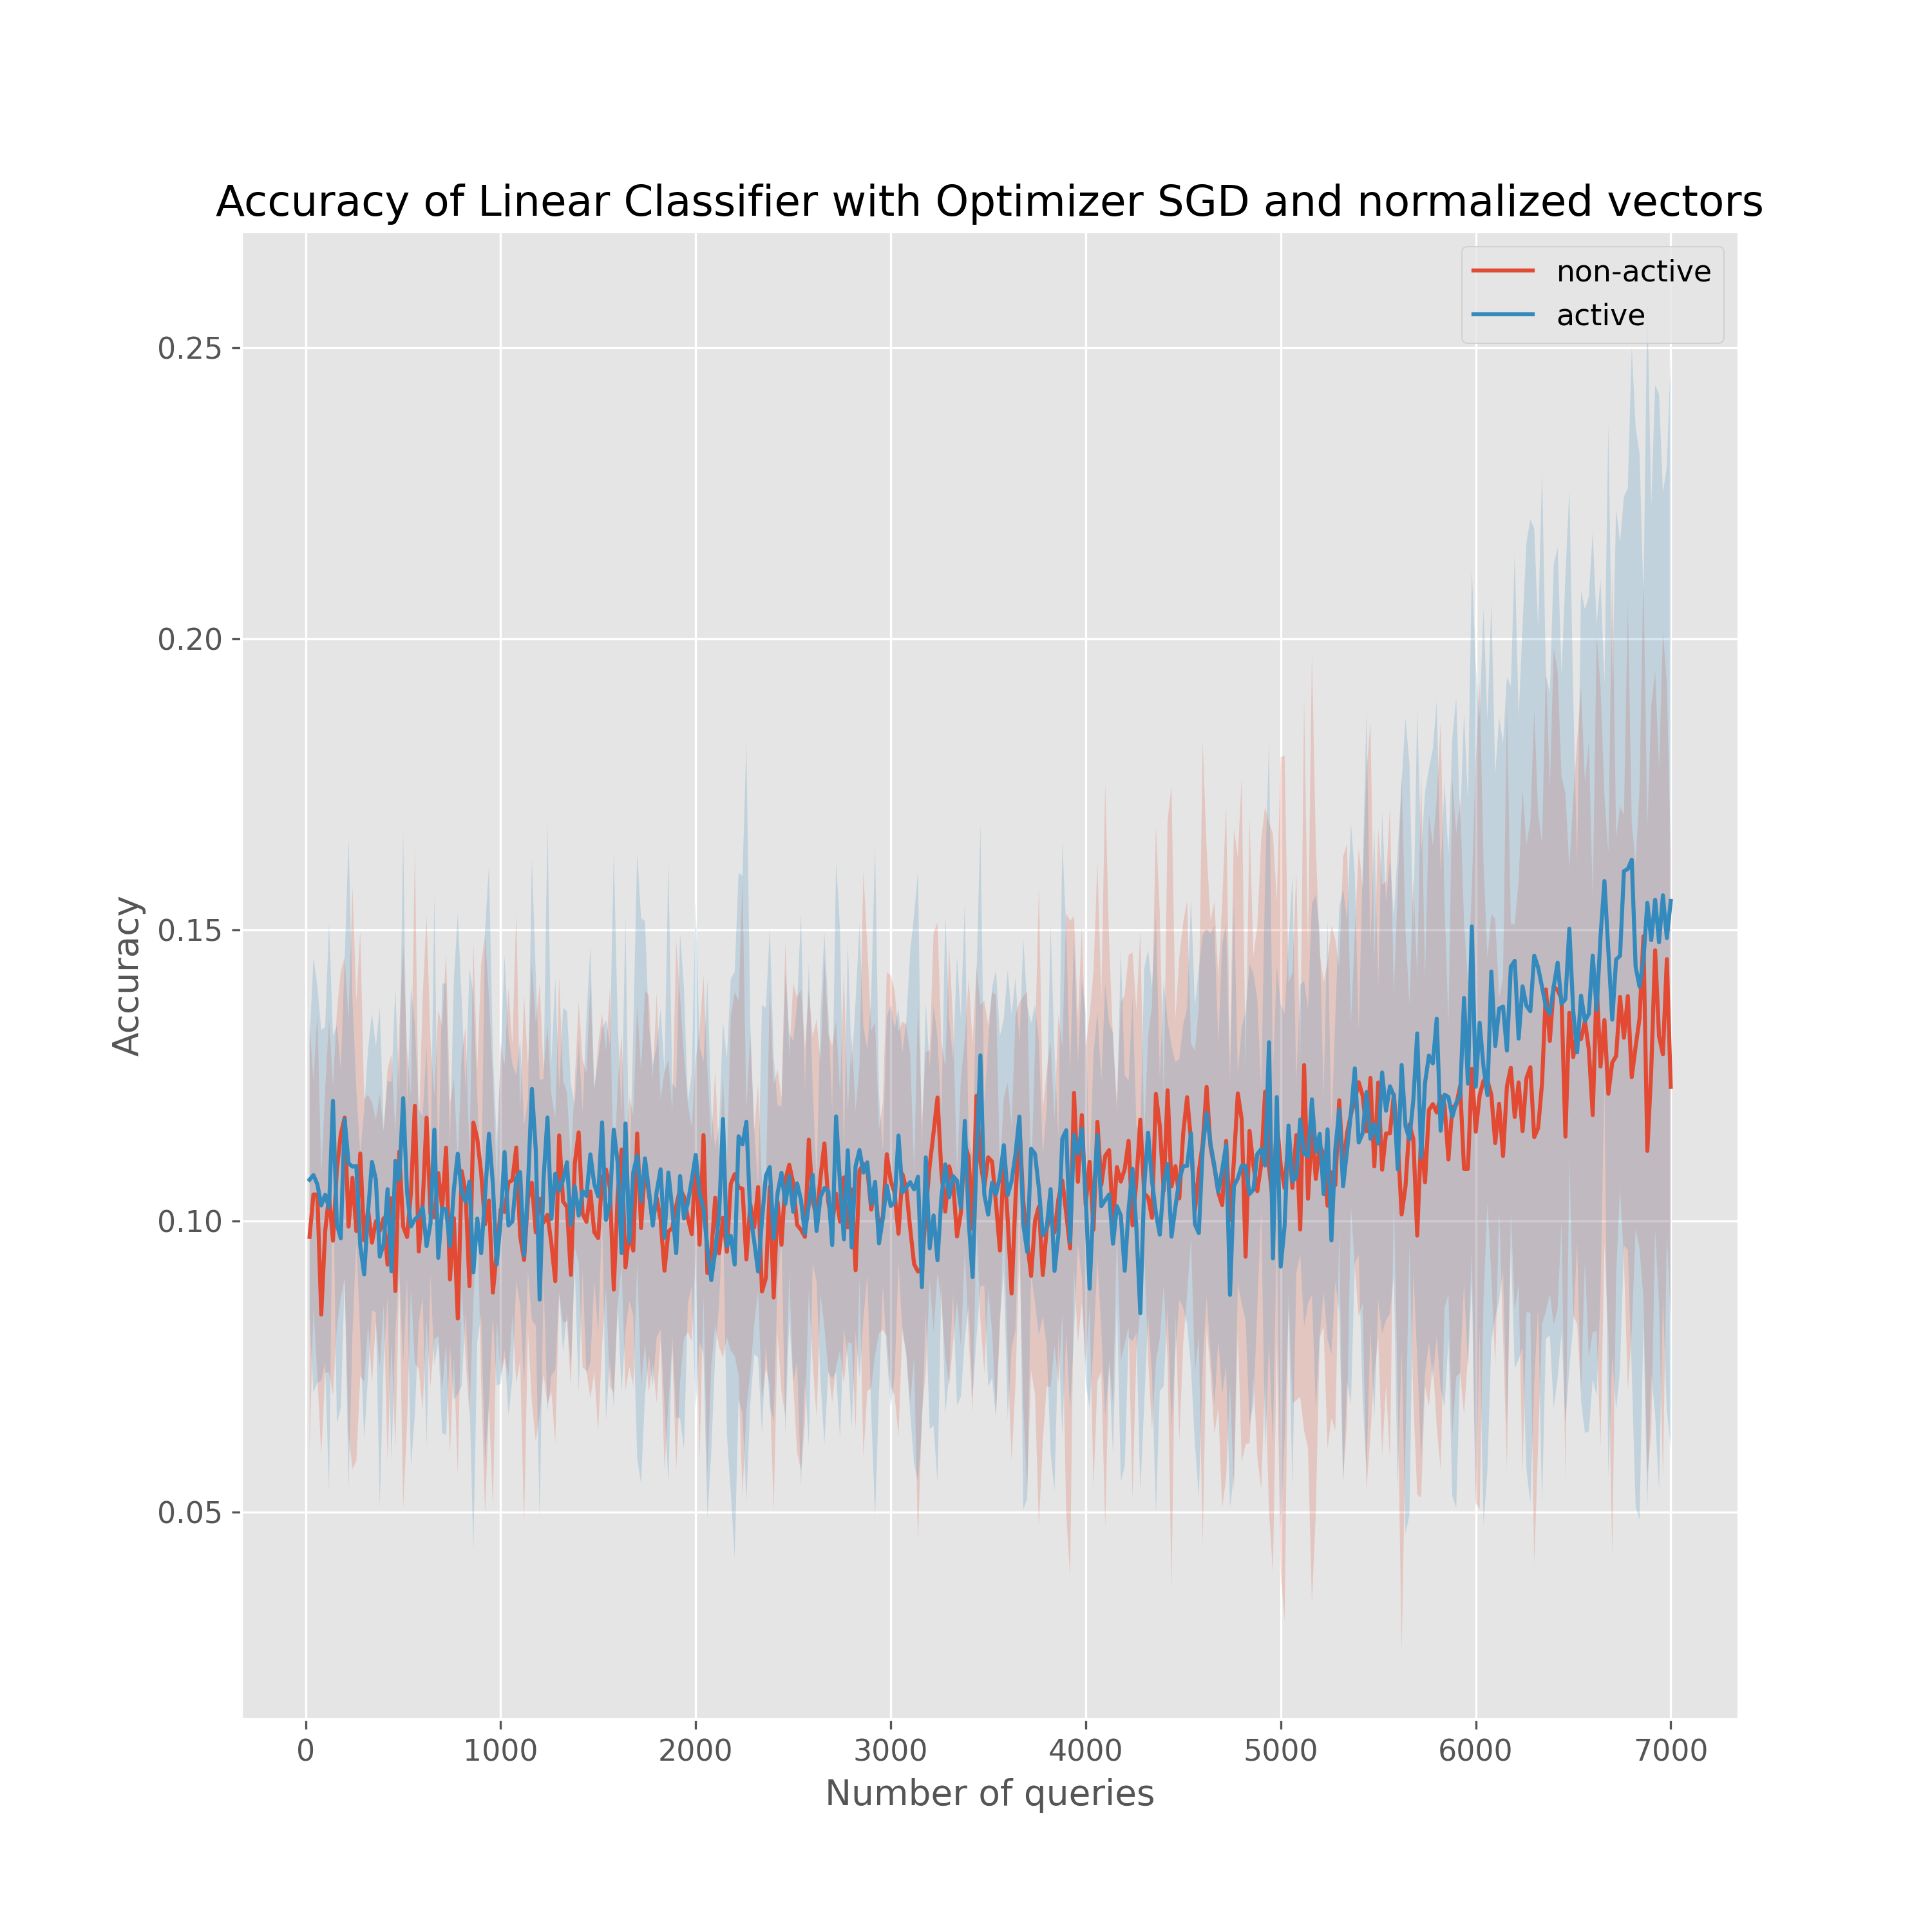
\includegraphics[width=\linewidth]{active-vs-base-mnist-linear-loss-SGD-normalized-ci}
  \end{minipage}%
  \begin{minipage}{.45\textwidth}
    \centering
    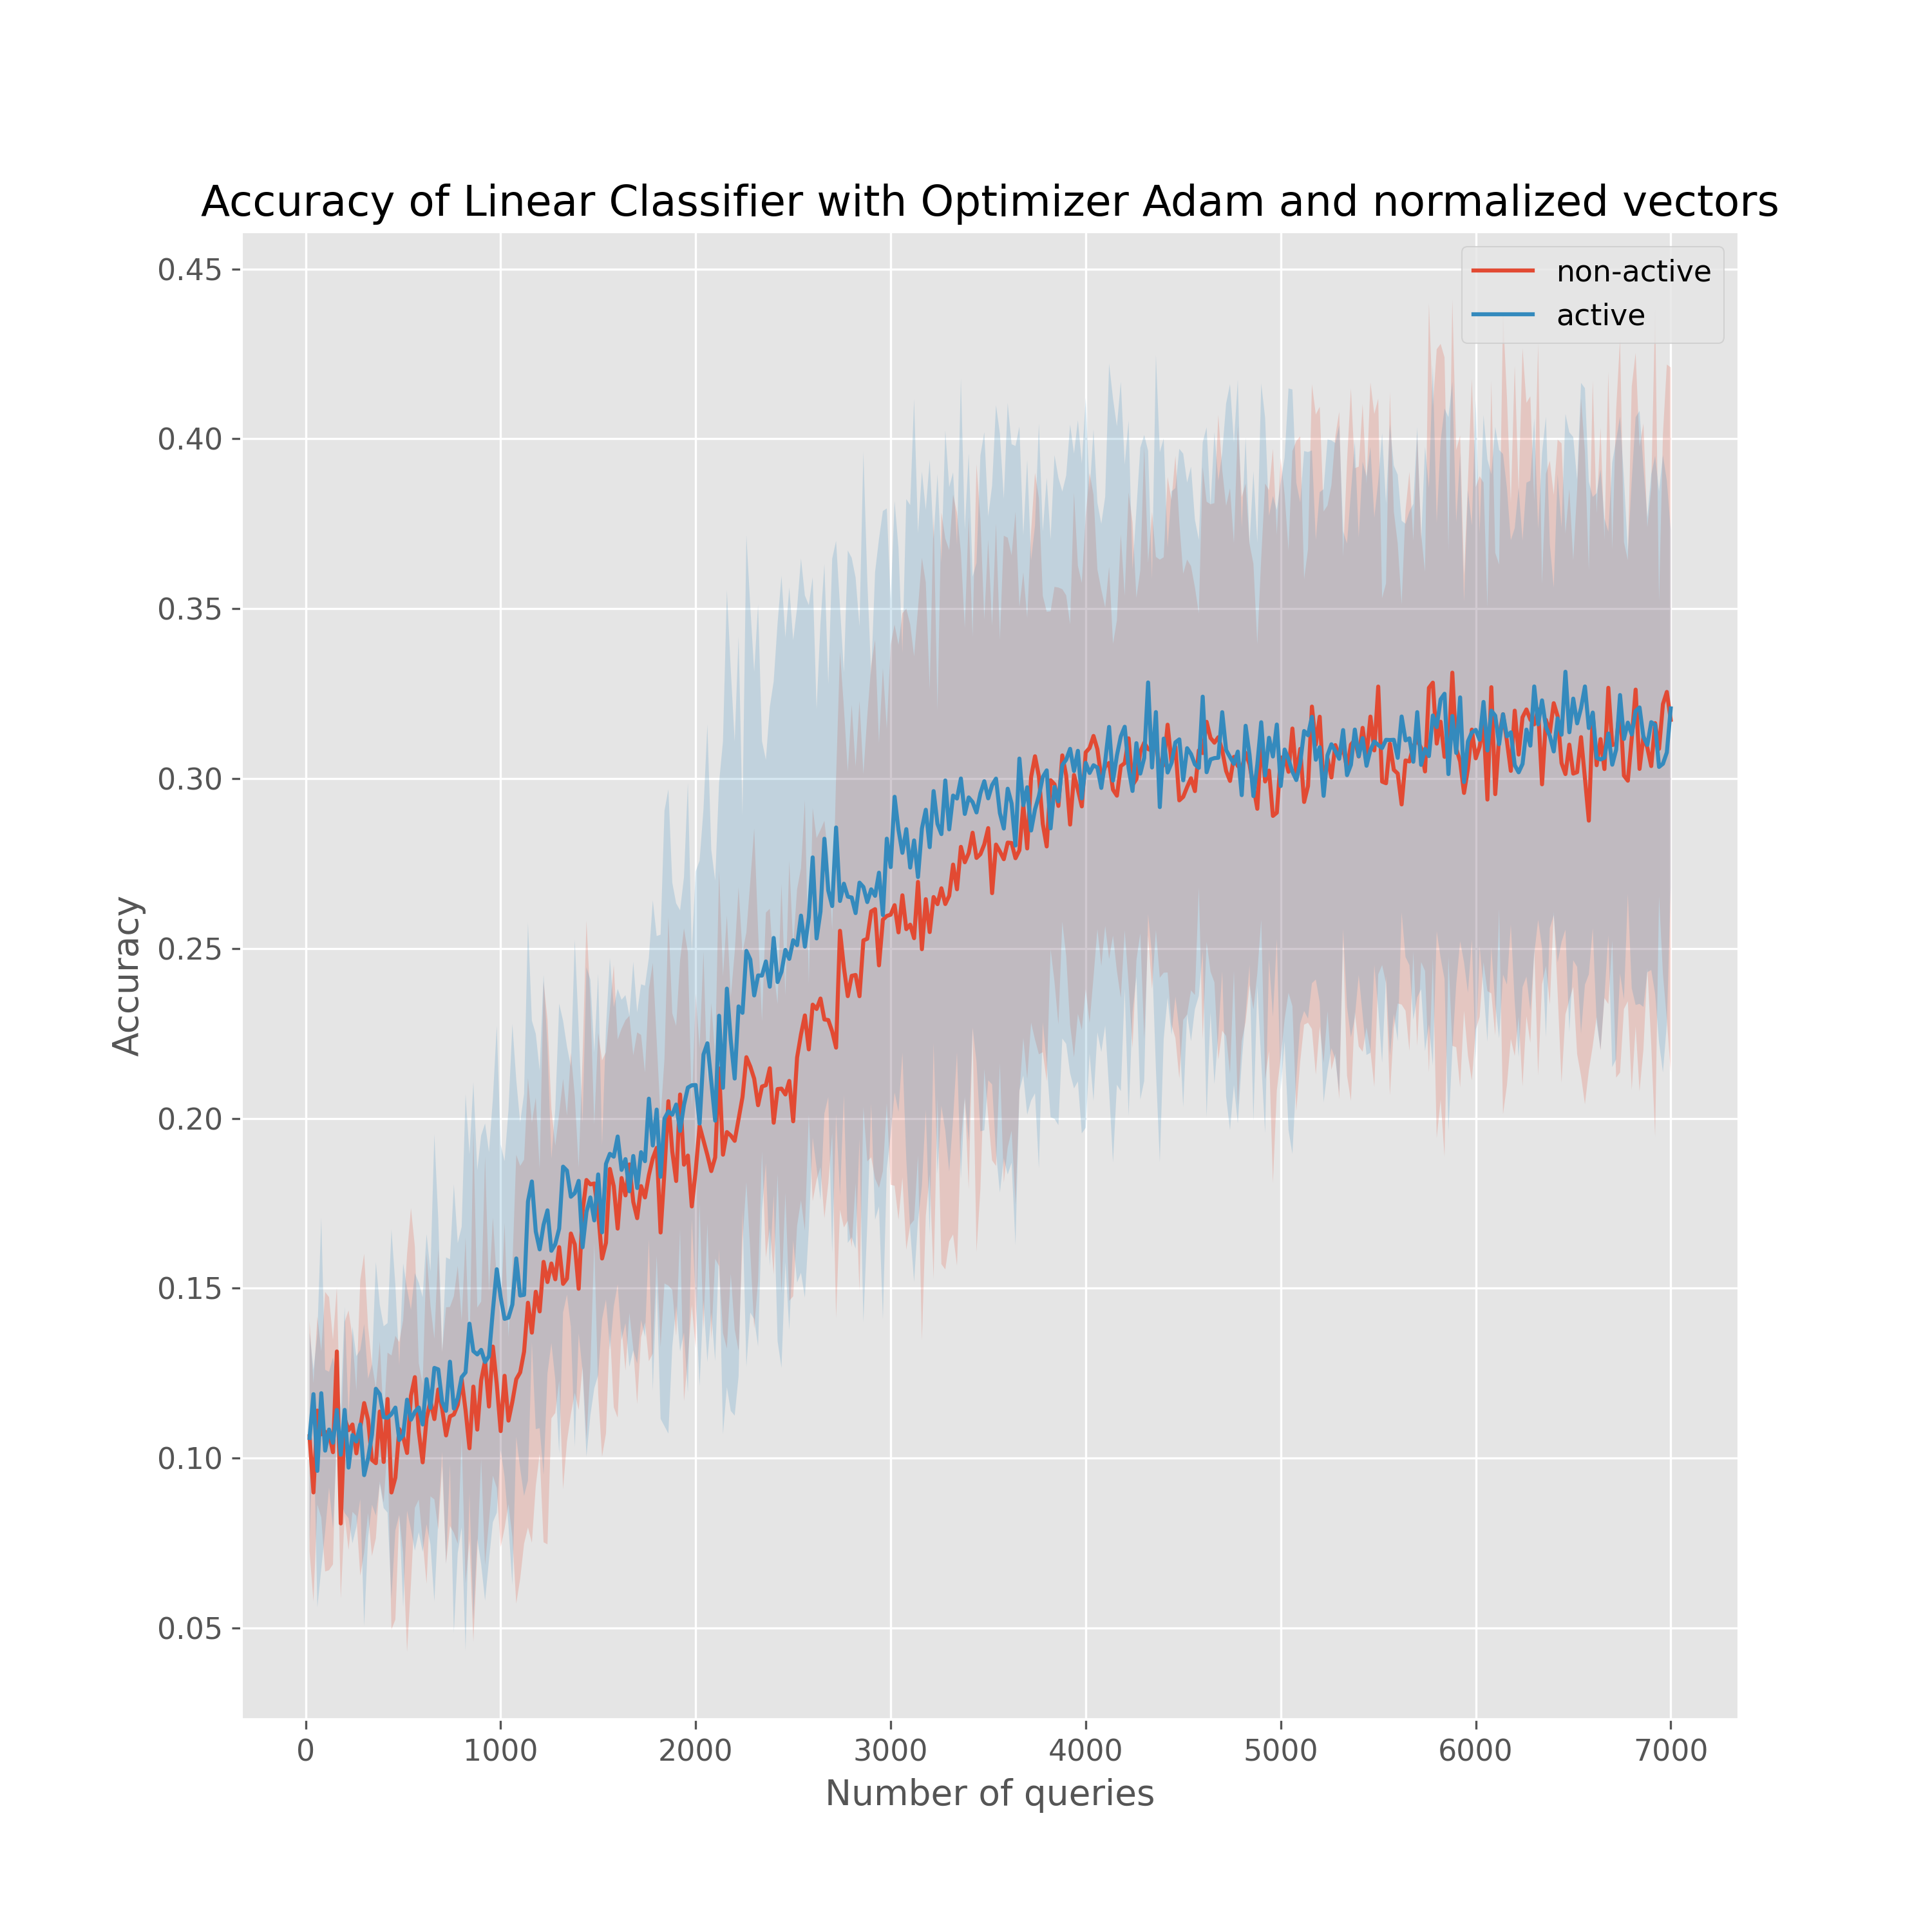
\includegraphics[width=\linewidth]{active-vs-base-mnist-linear-loss-Adam-normalized-ci}
  \end{minipage}
  \caption{Performance SVM on normalized learned features SGD (left) vs Adam (right)}\label{fig:svm-normalized-ci-mnist}
\end{figure}


\begin{figure}[!h]
  \centering
  \begin{minipage}{.45\textwidth}
    \centering
    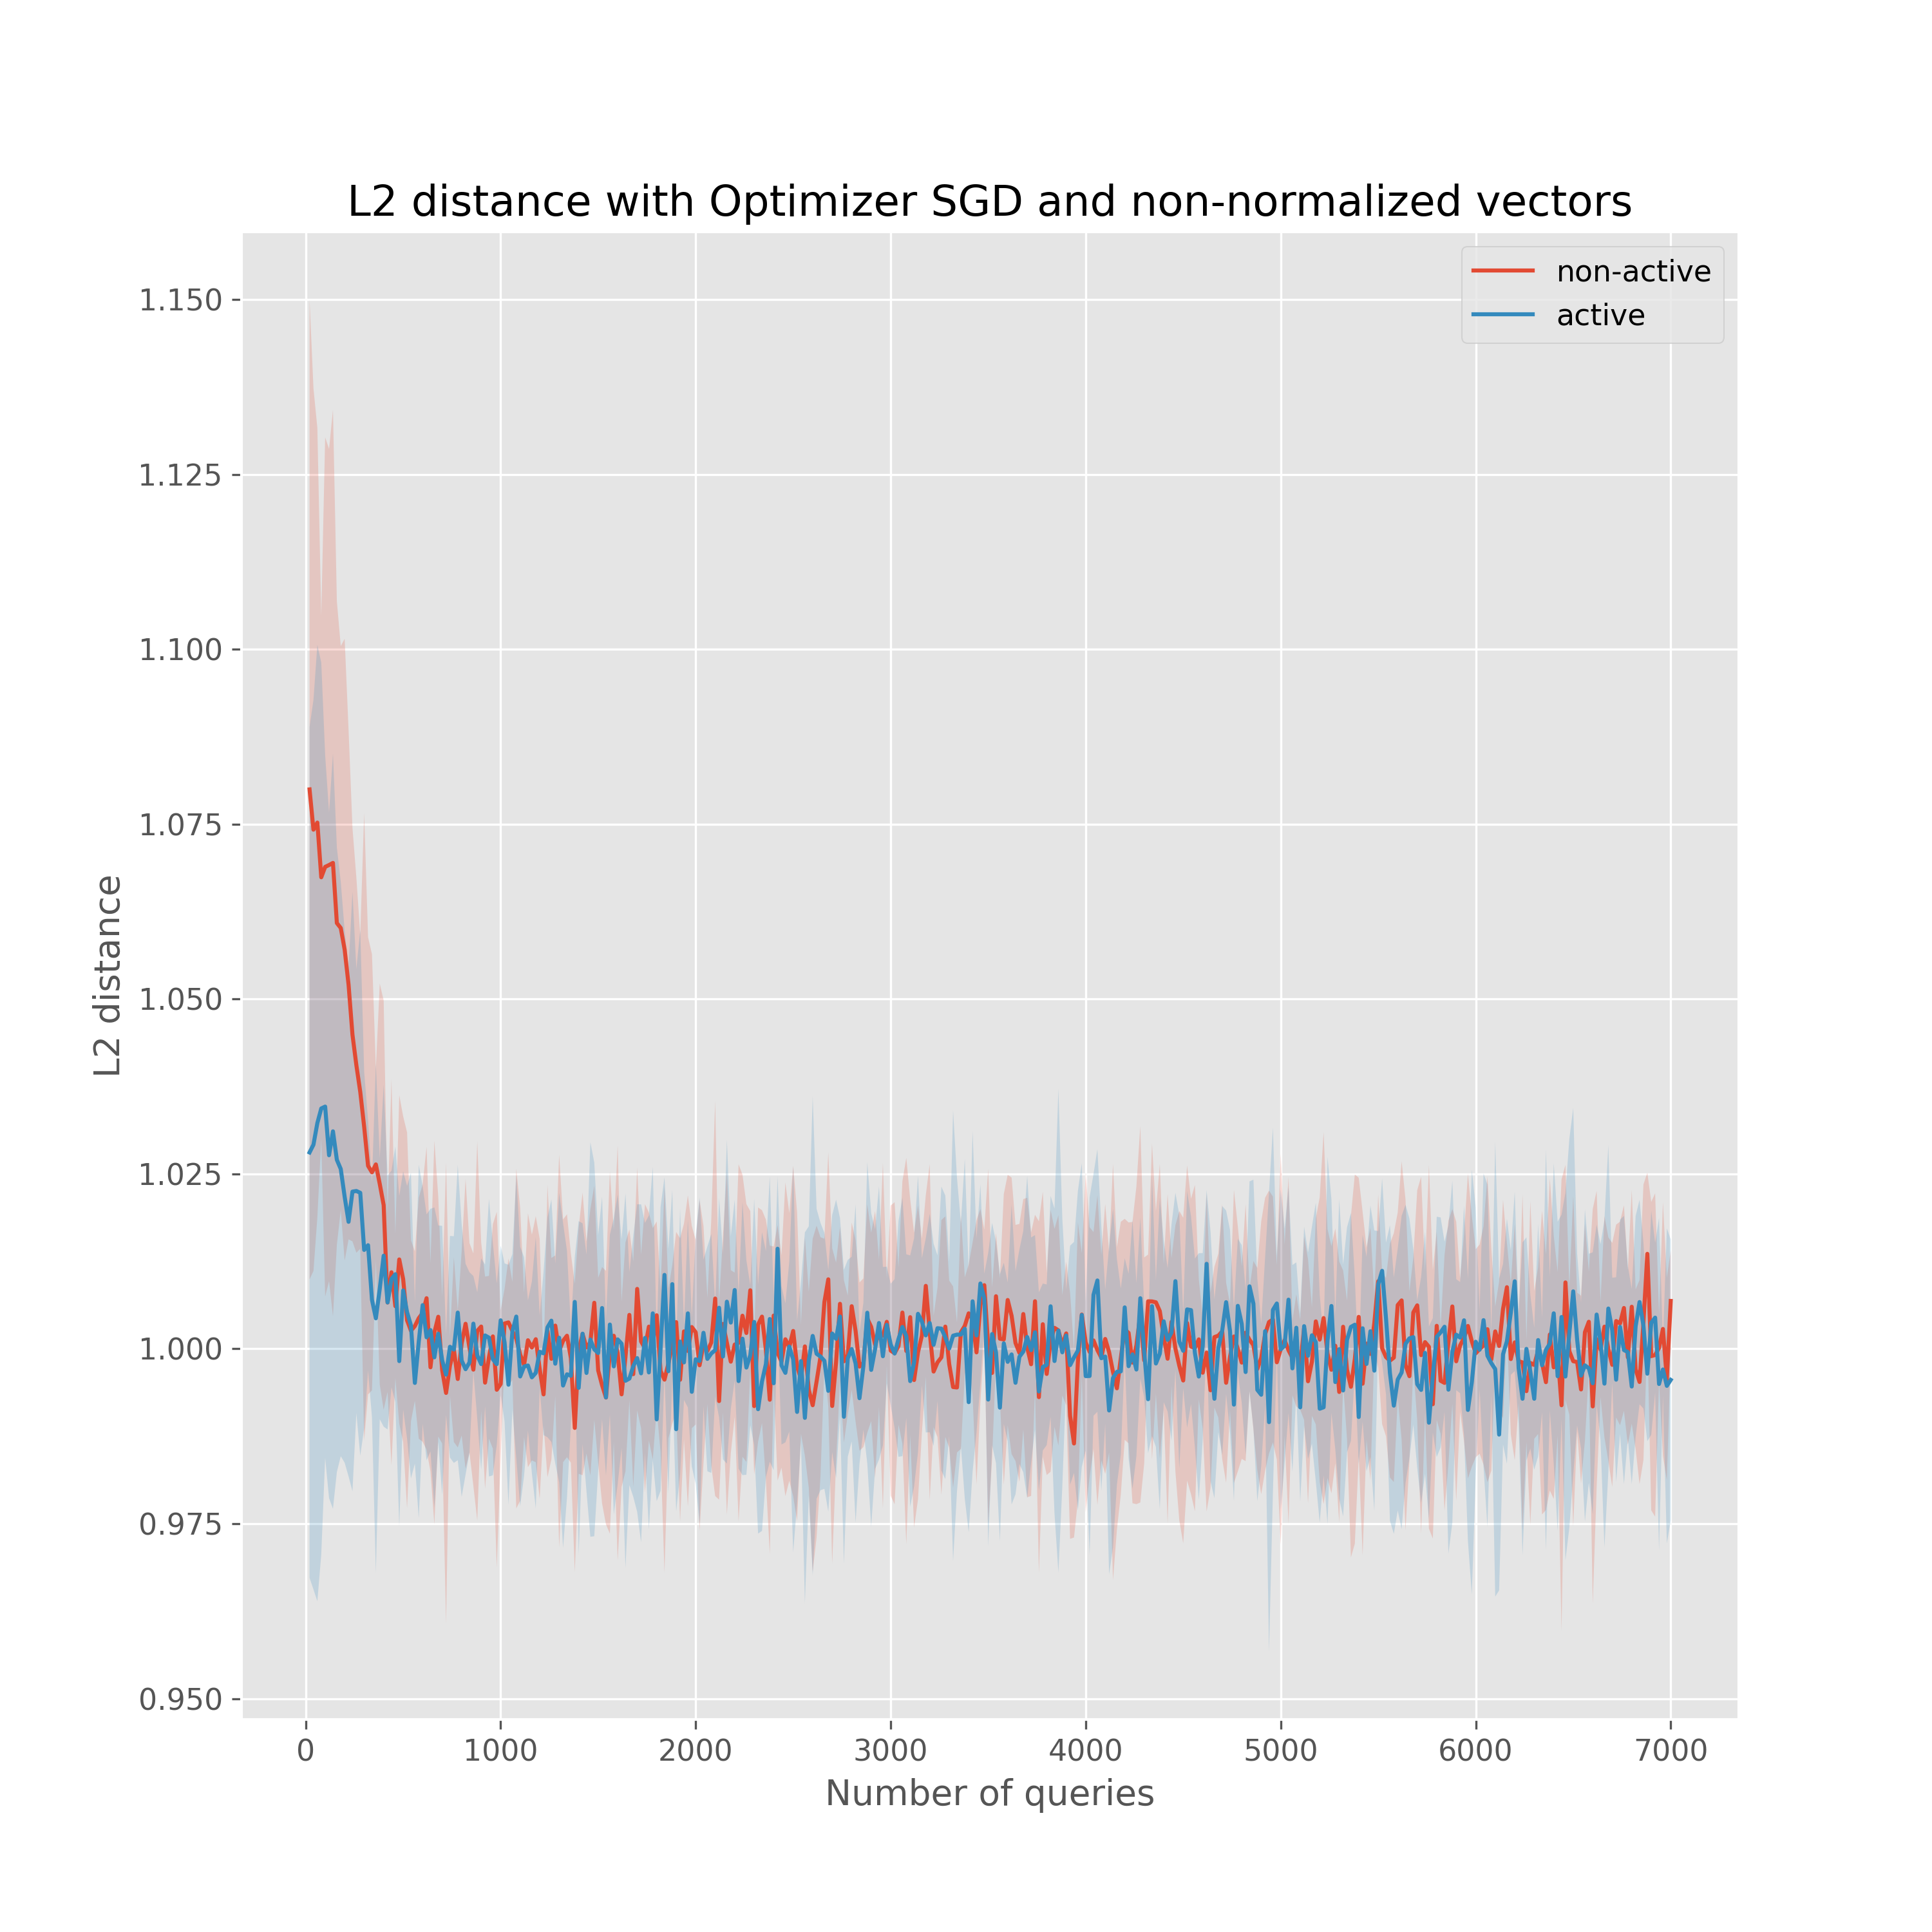
\includegraphics[width=\linewidth]{active-vs-base-mnist-l2-loss-SGD-non-normalized-ci}
  \end{minipage}%
  \begin{minipage}{.45\textwidth}
    \centering
    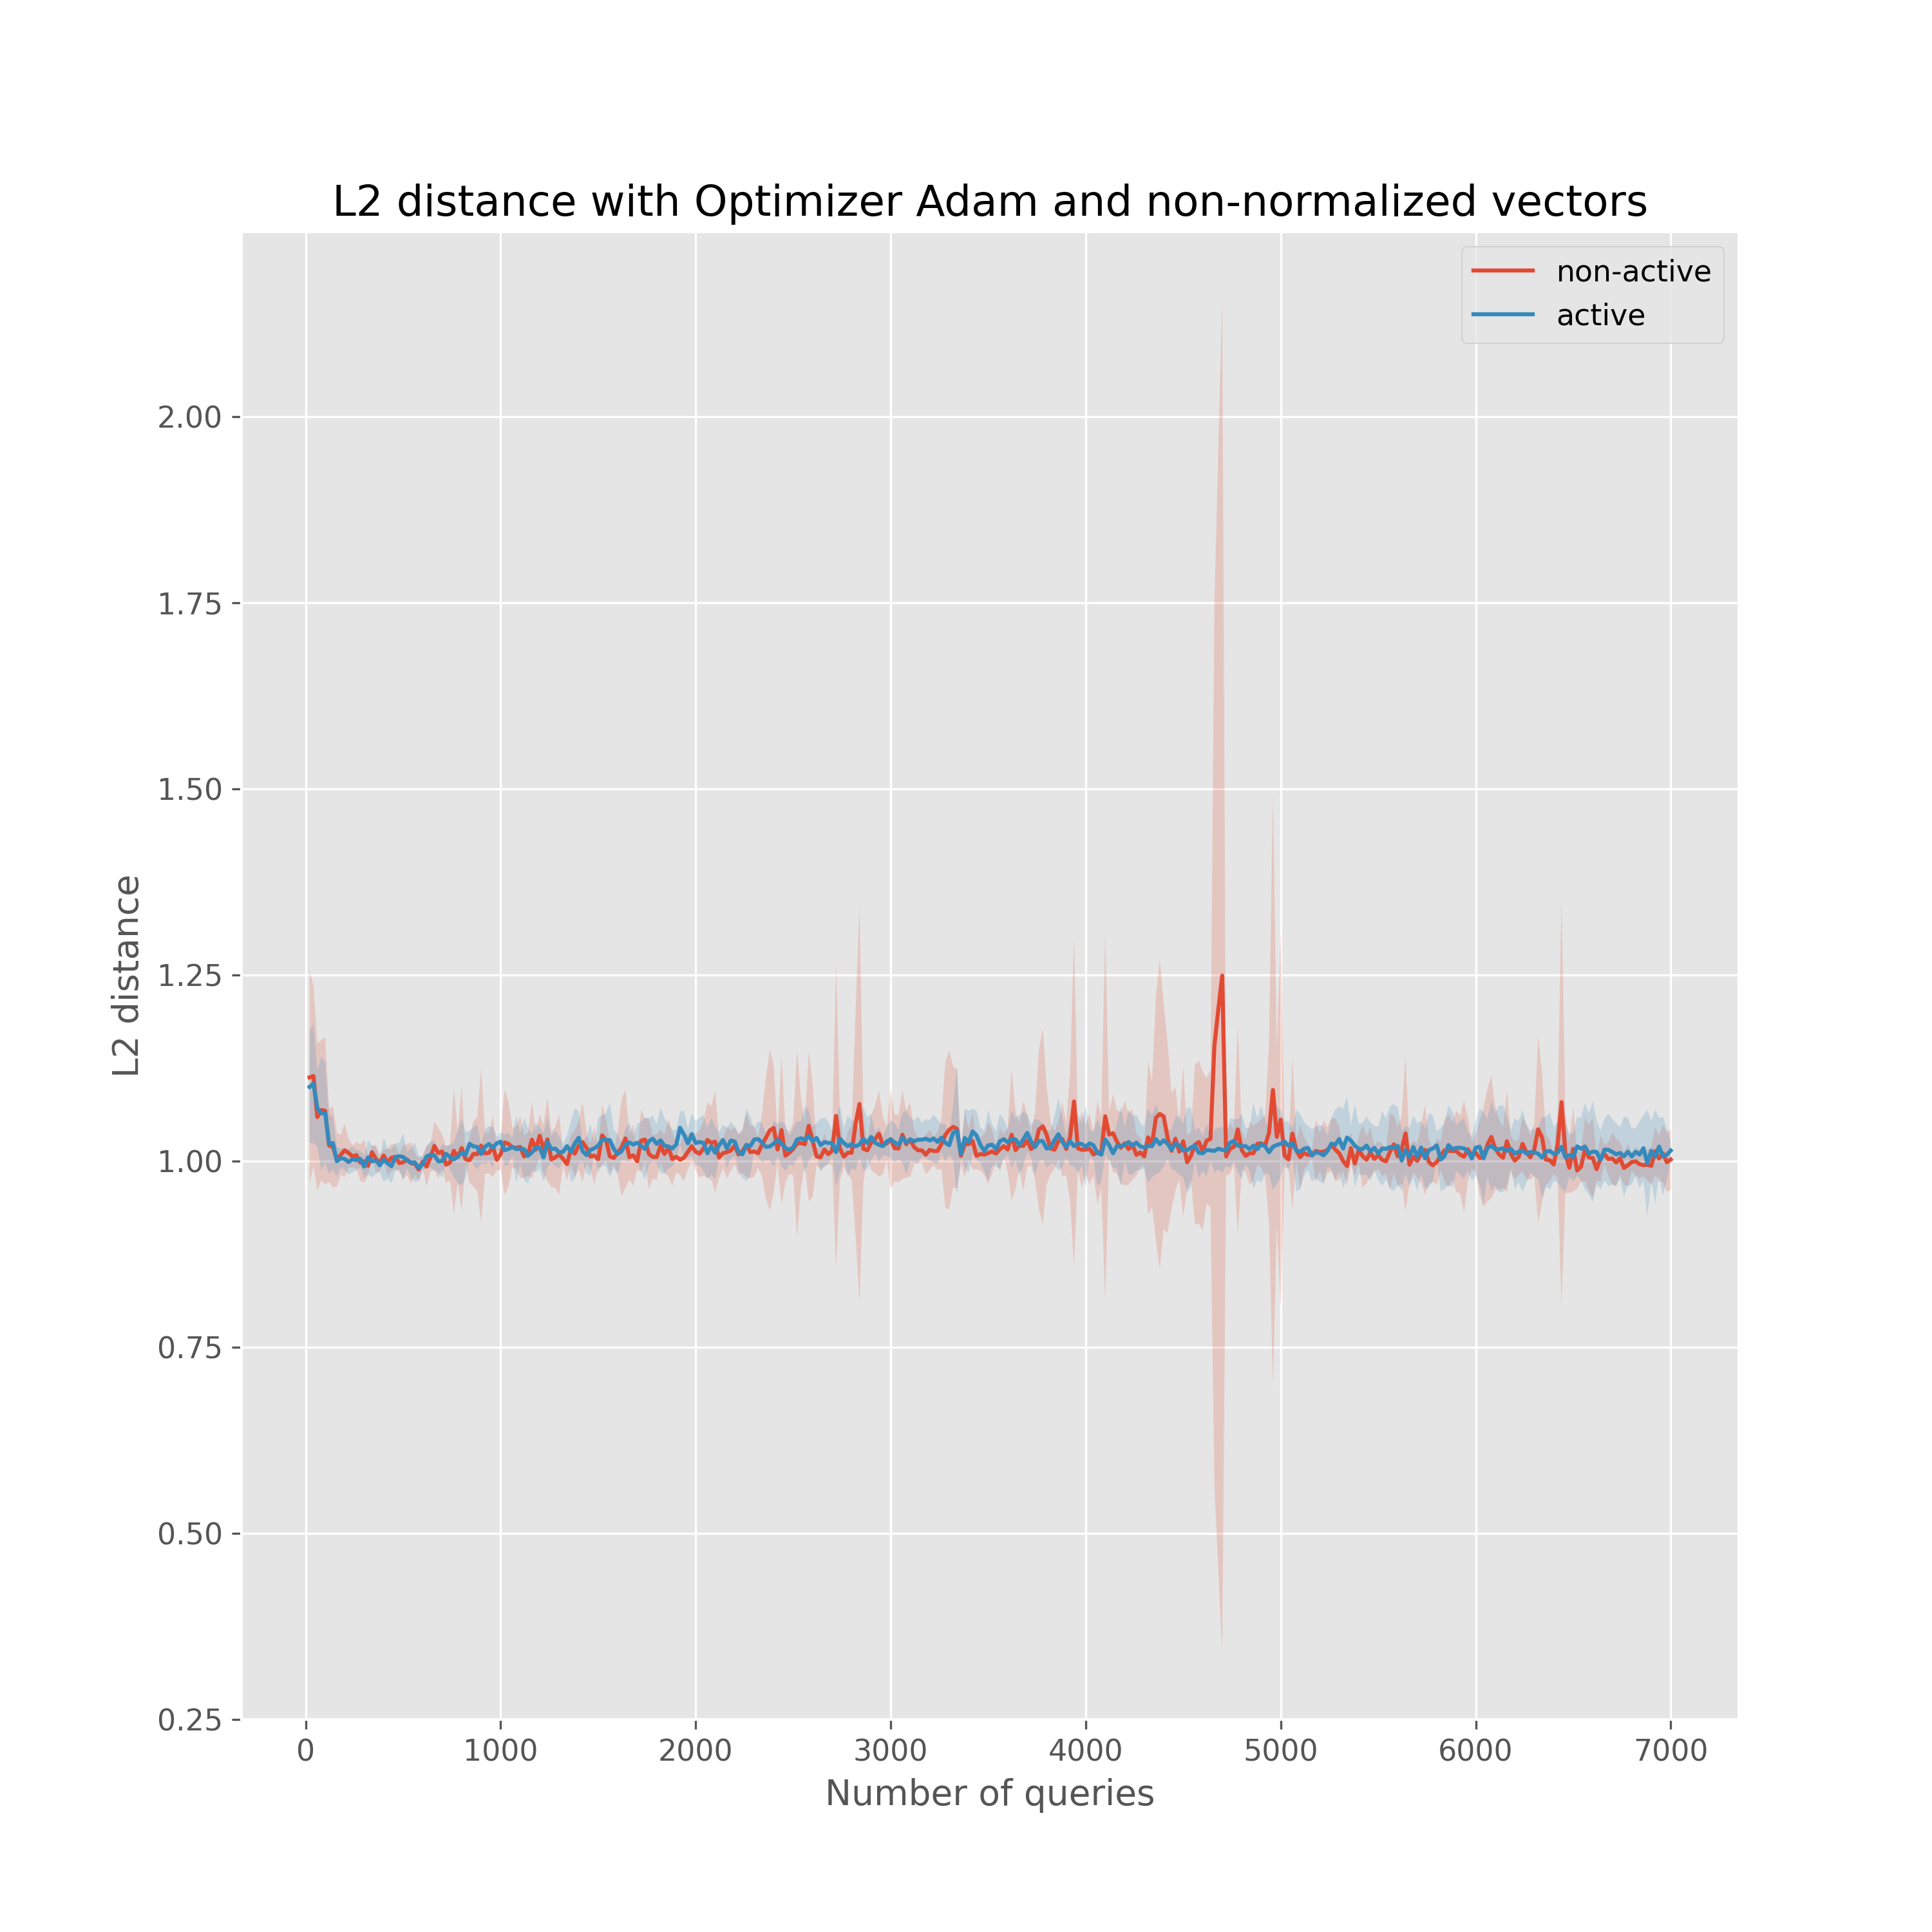
\includegraphics[width=\linewidth]{active-vs-base-mnist-l2-loss-Adam-non-normalized-ci}
  \end{minipage}
  \caption{$l_2$ loss on non-normalized features SGD (left) vs Adam (right)}\label{fig:l2-loss-non-normalized-ci-mnist}
\end{figure}

% add figures
\begin{figure}[h]
  \centering
  \begin{minipage}{.45\textwidth}
    \centering
    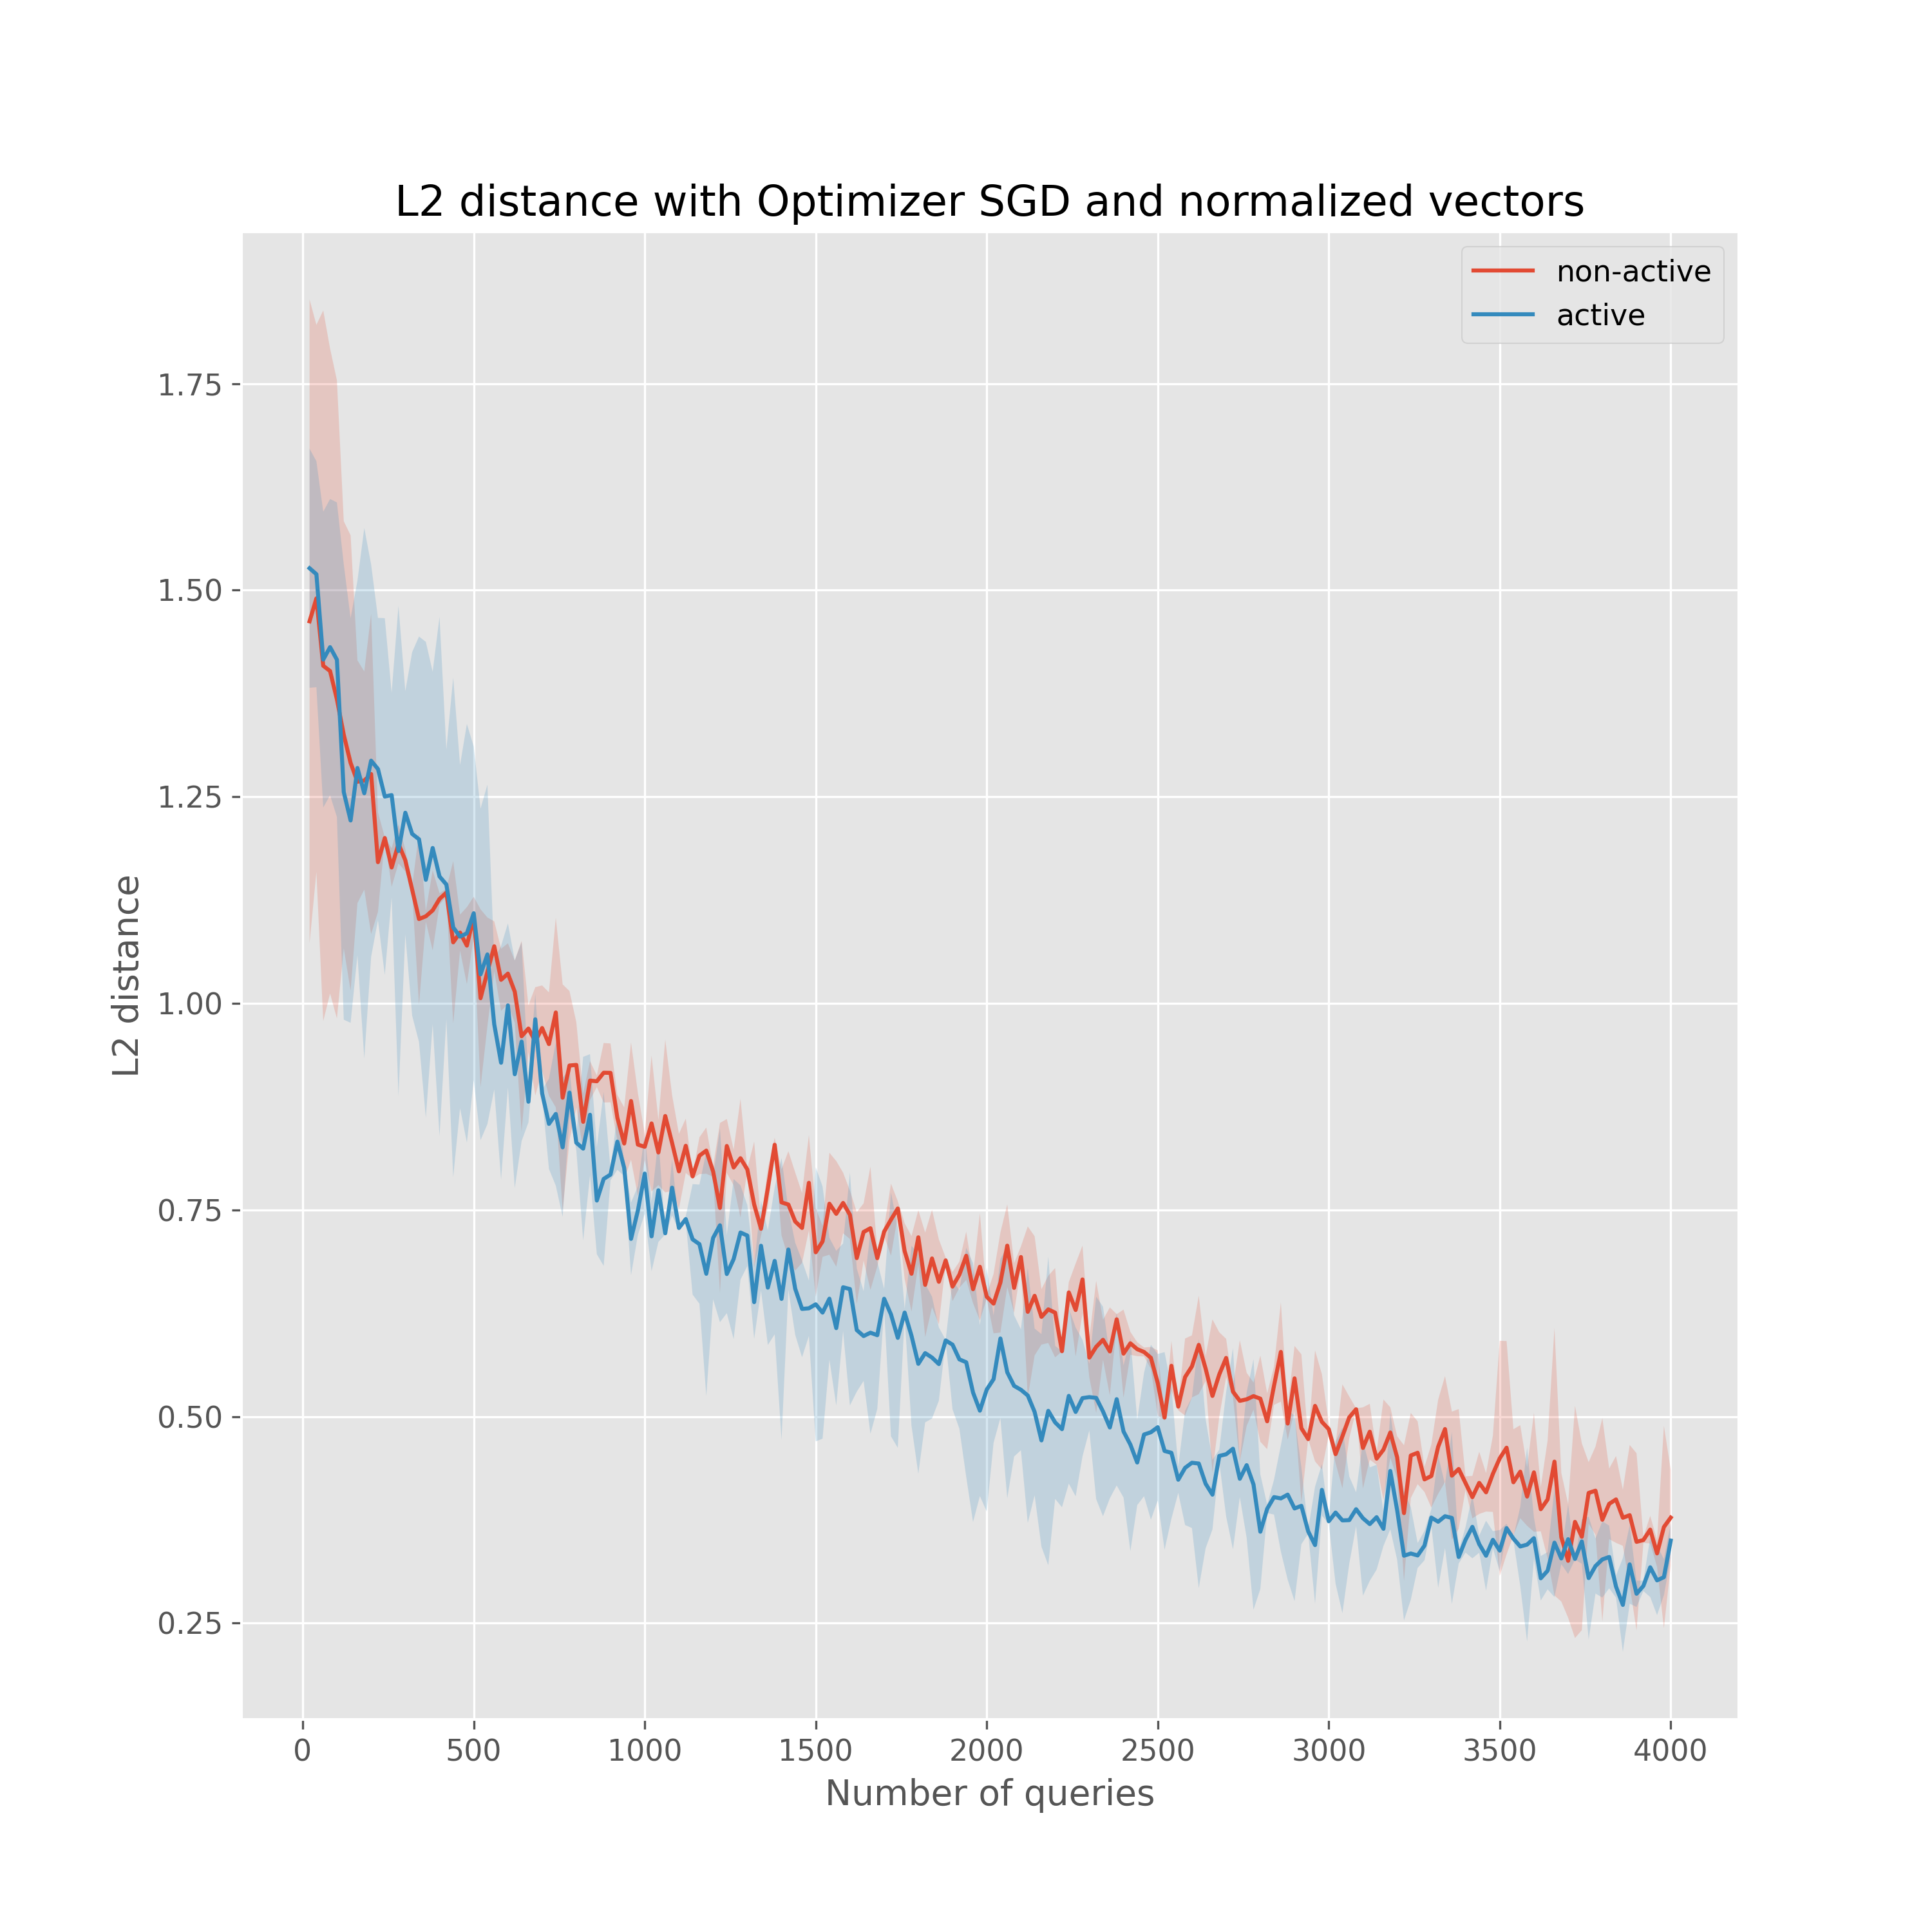
\includegraphics[width=\linewidth]{active-vs-base-moons-l2-loss-SGD-normalized-ci}
  \end{minipage}%
  \begin{minipage}{.45\textwidth}
    \centering
    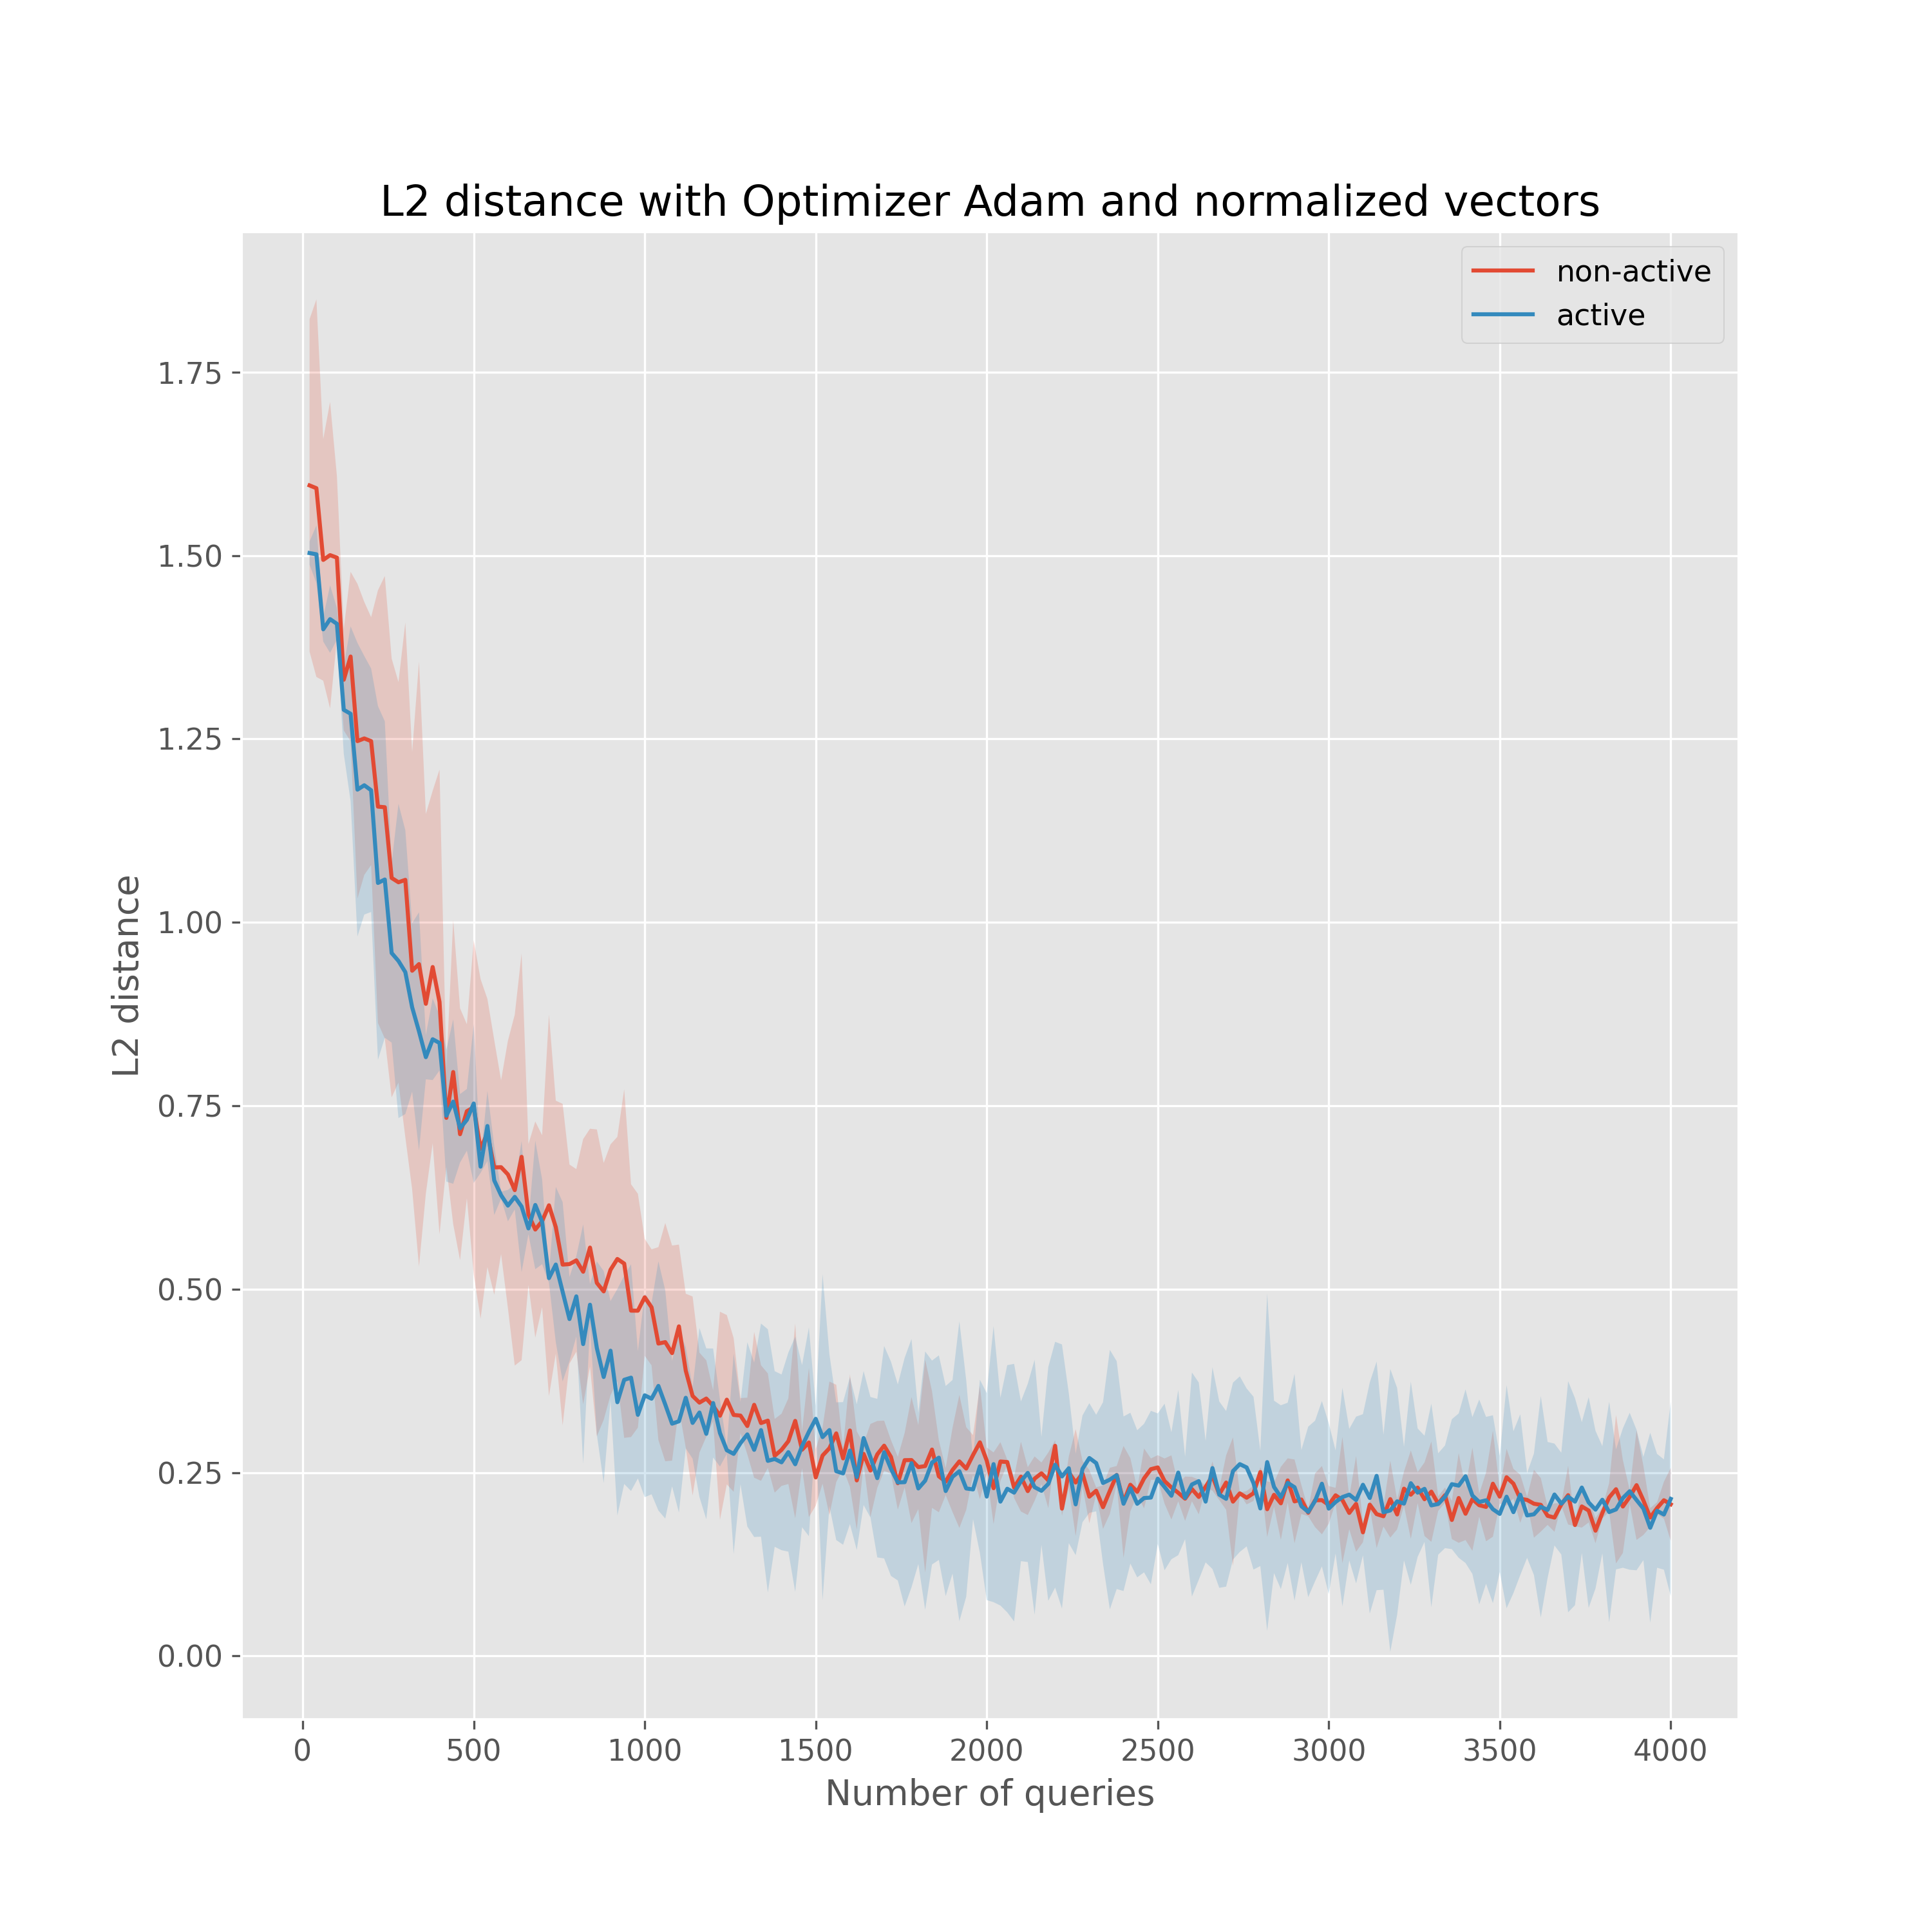
\includegraphics[width=\linewidth]{active-vs-base-moons-l2-loss-Adam-normalized-ci}
  \end{minipage}
  \caption{$l_2$ loss on normalized features SGD (left) vs Adam (right)}\label{fig:l2-loss-normalized-ci-mnist}
\end{figure}

% add figures
\begin{figure}[h]
  \centering
  \begin{minipage}{.45\textwidth}
    \centering
    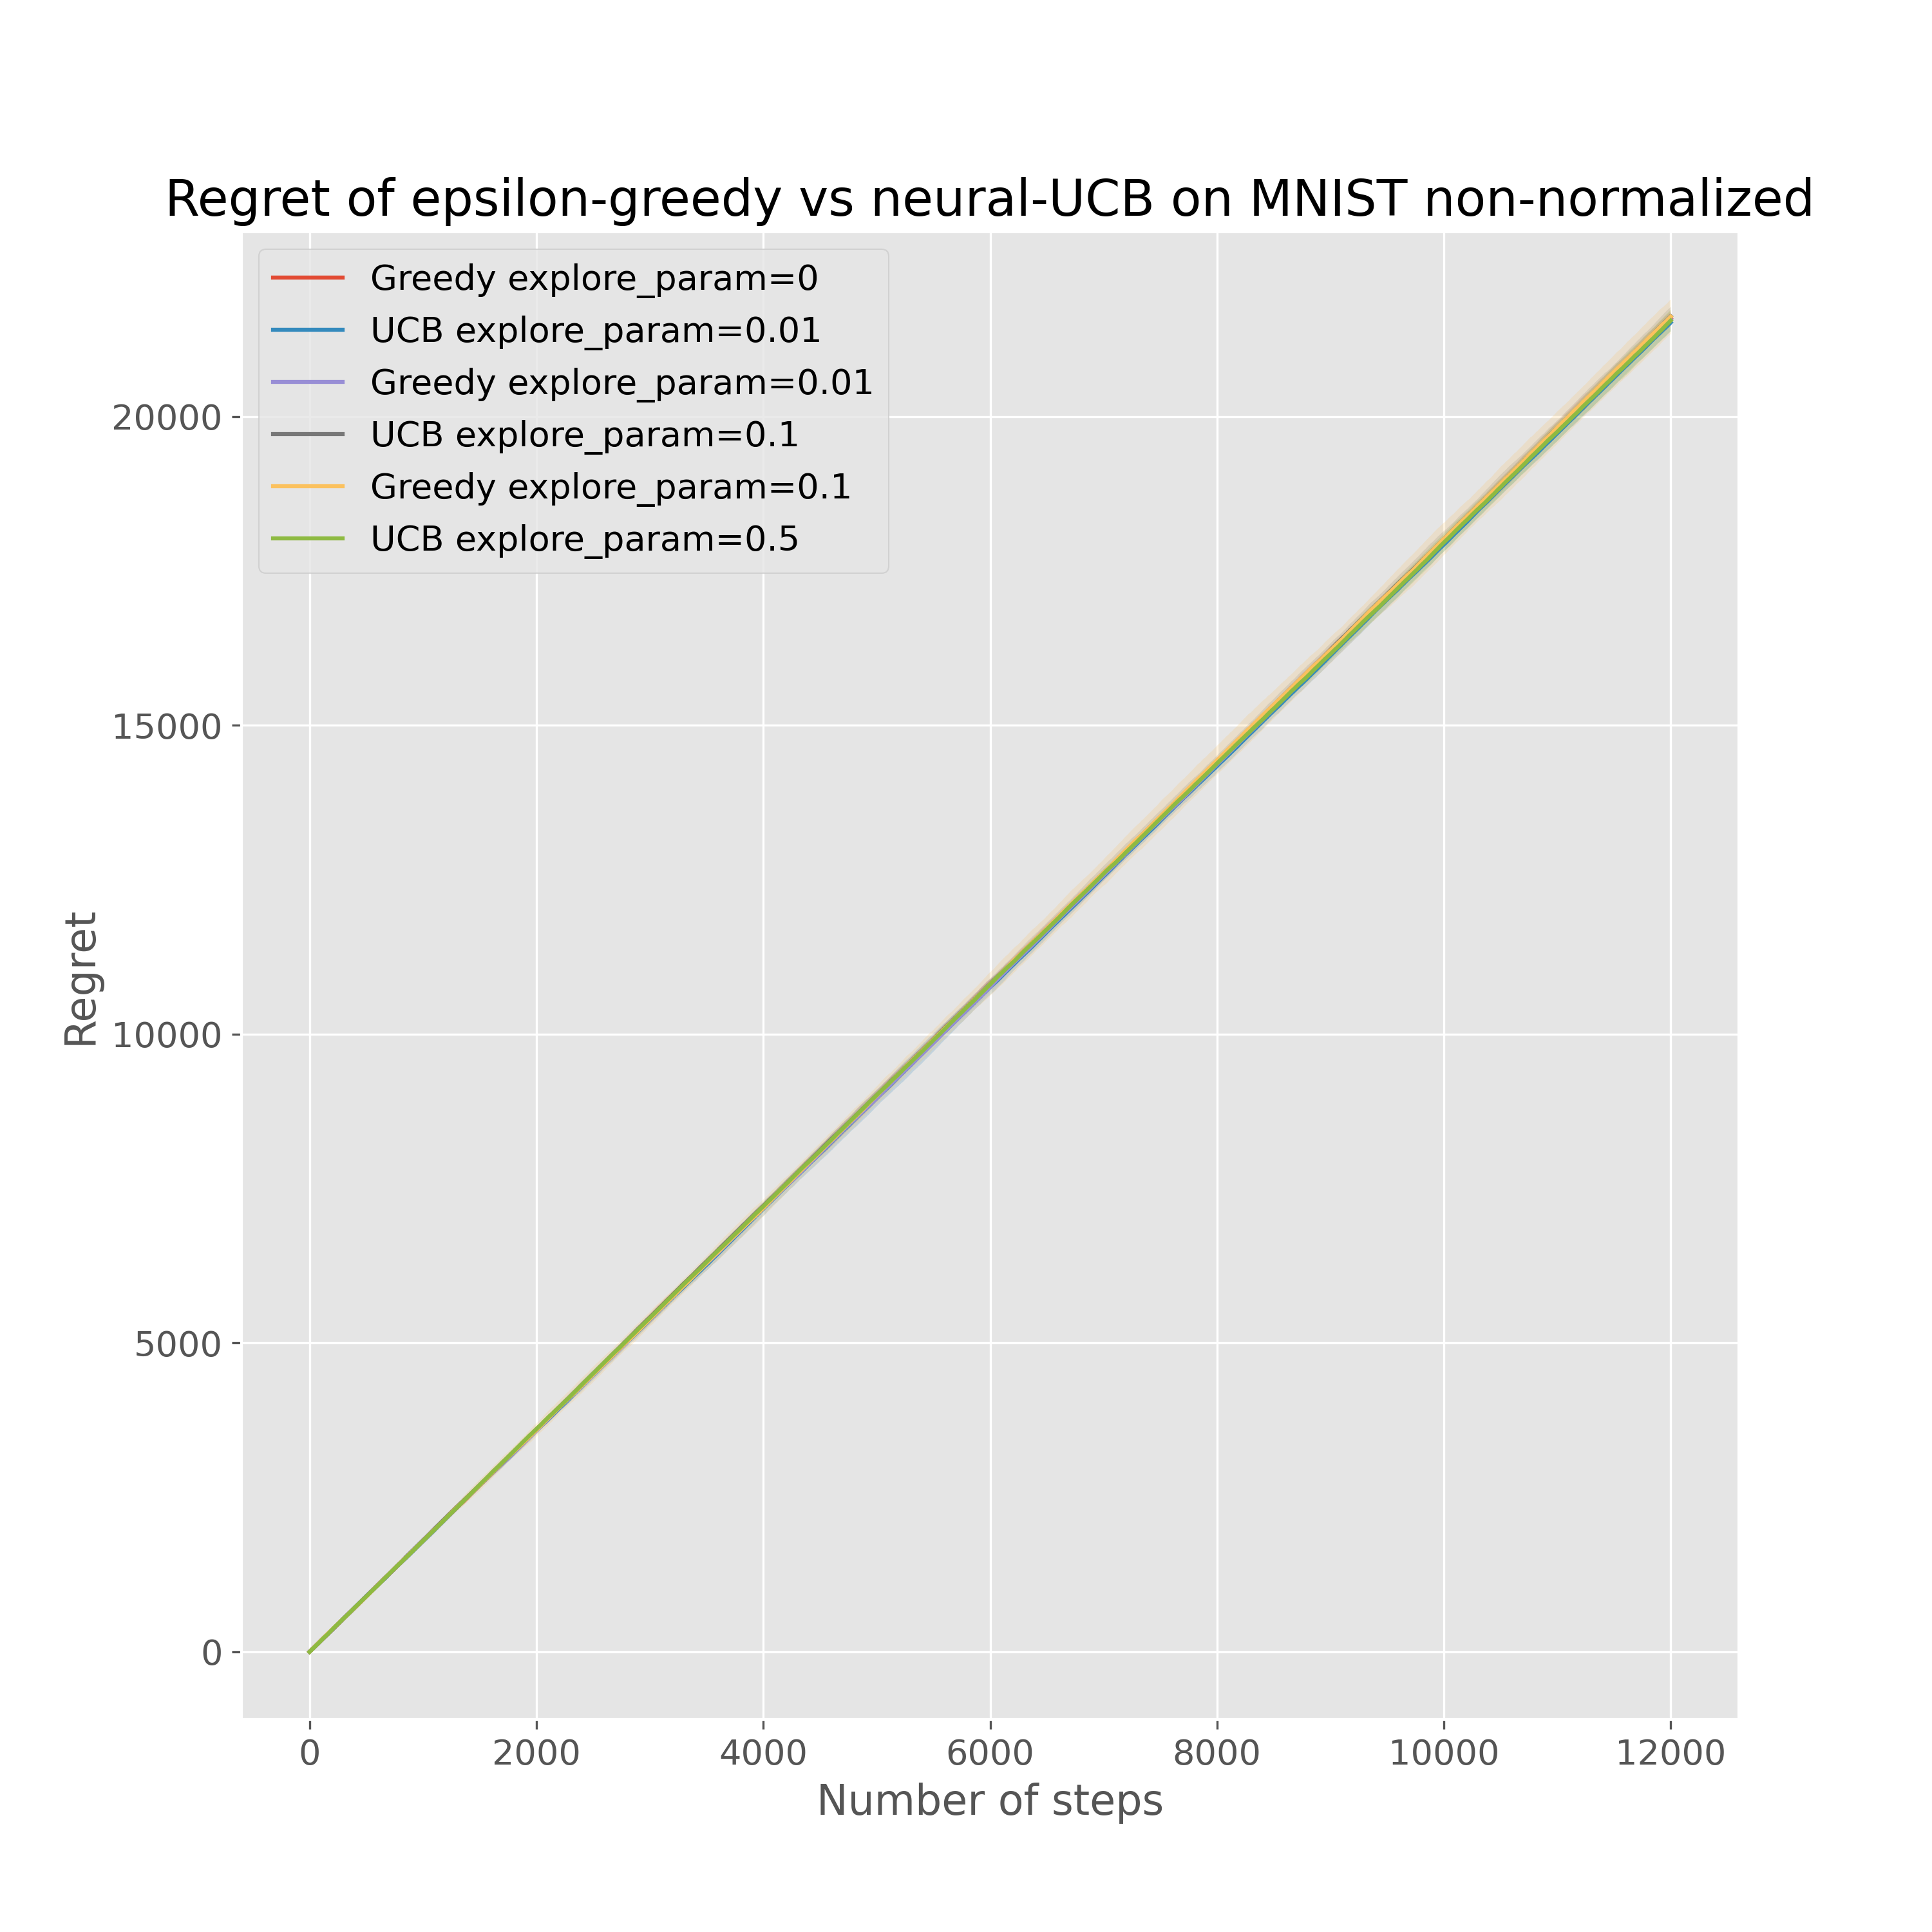
\includegraphics[width=\linewidth]{online-epsilon-vs-neural-mnist--non-normalized-ci}
  \end{minipage}%
  \begin{minipage}{.45\textwidth}
    \centering
    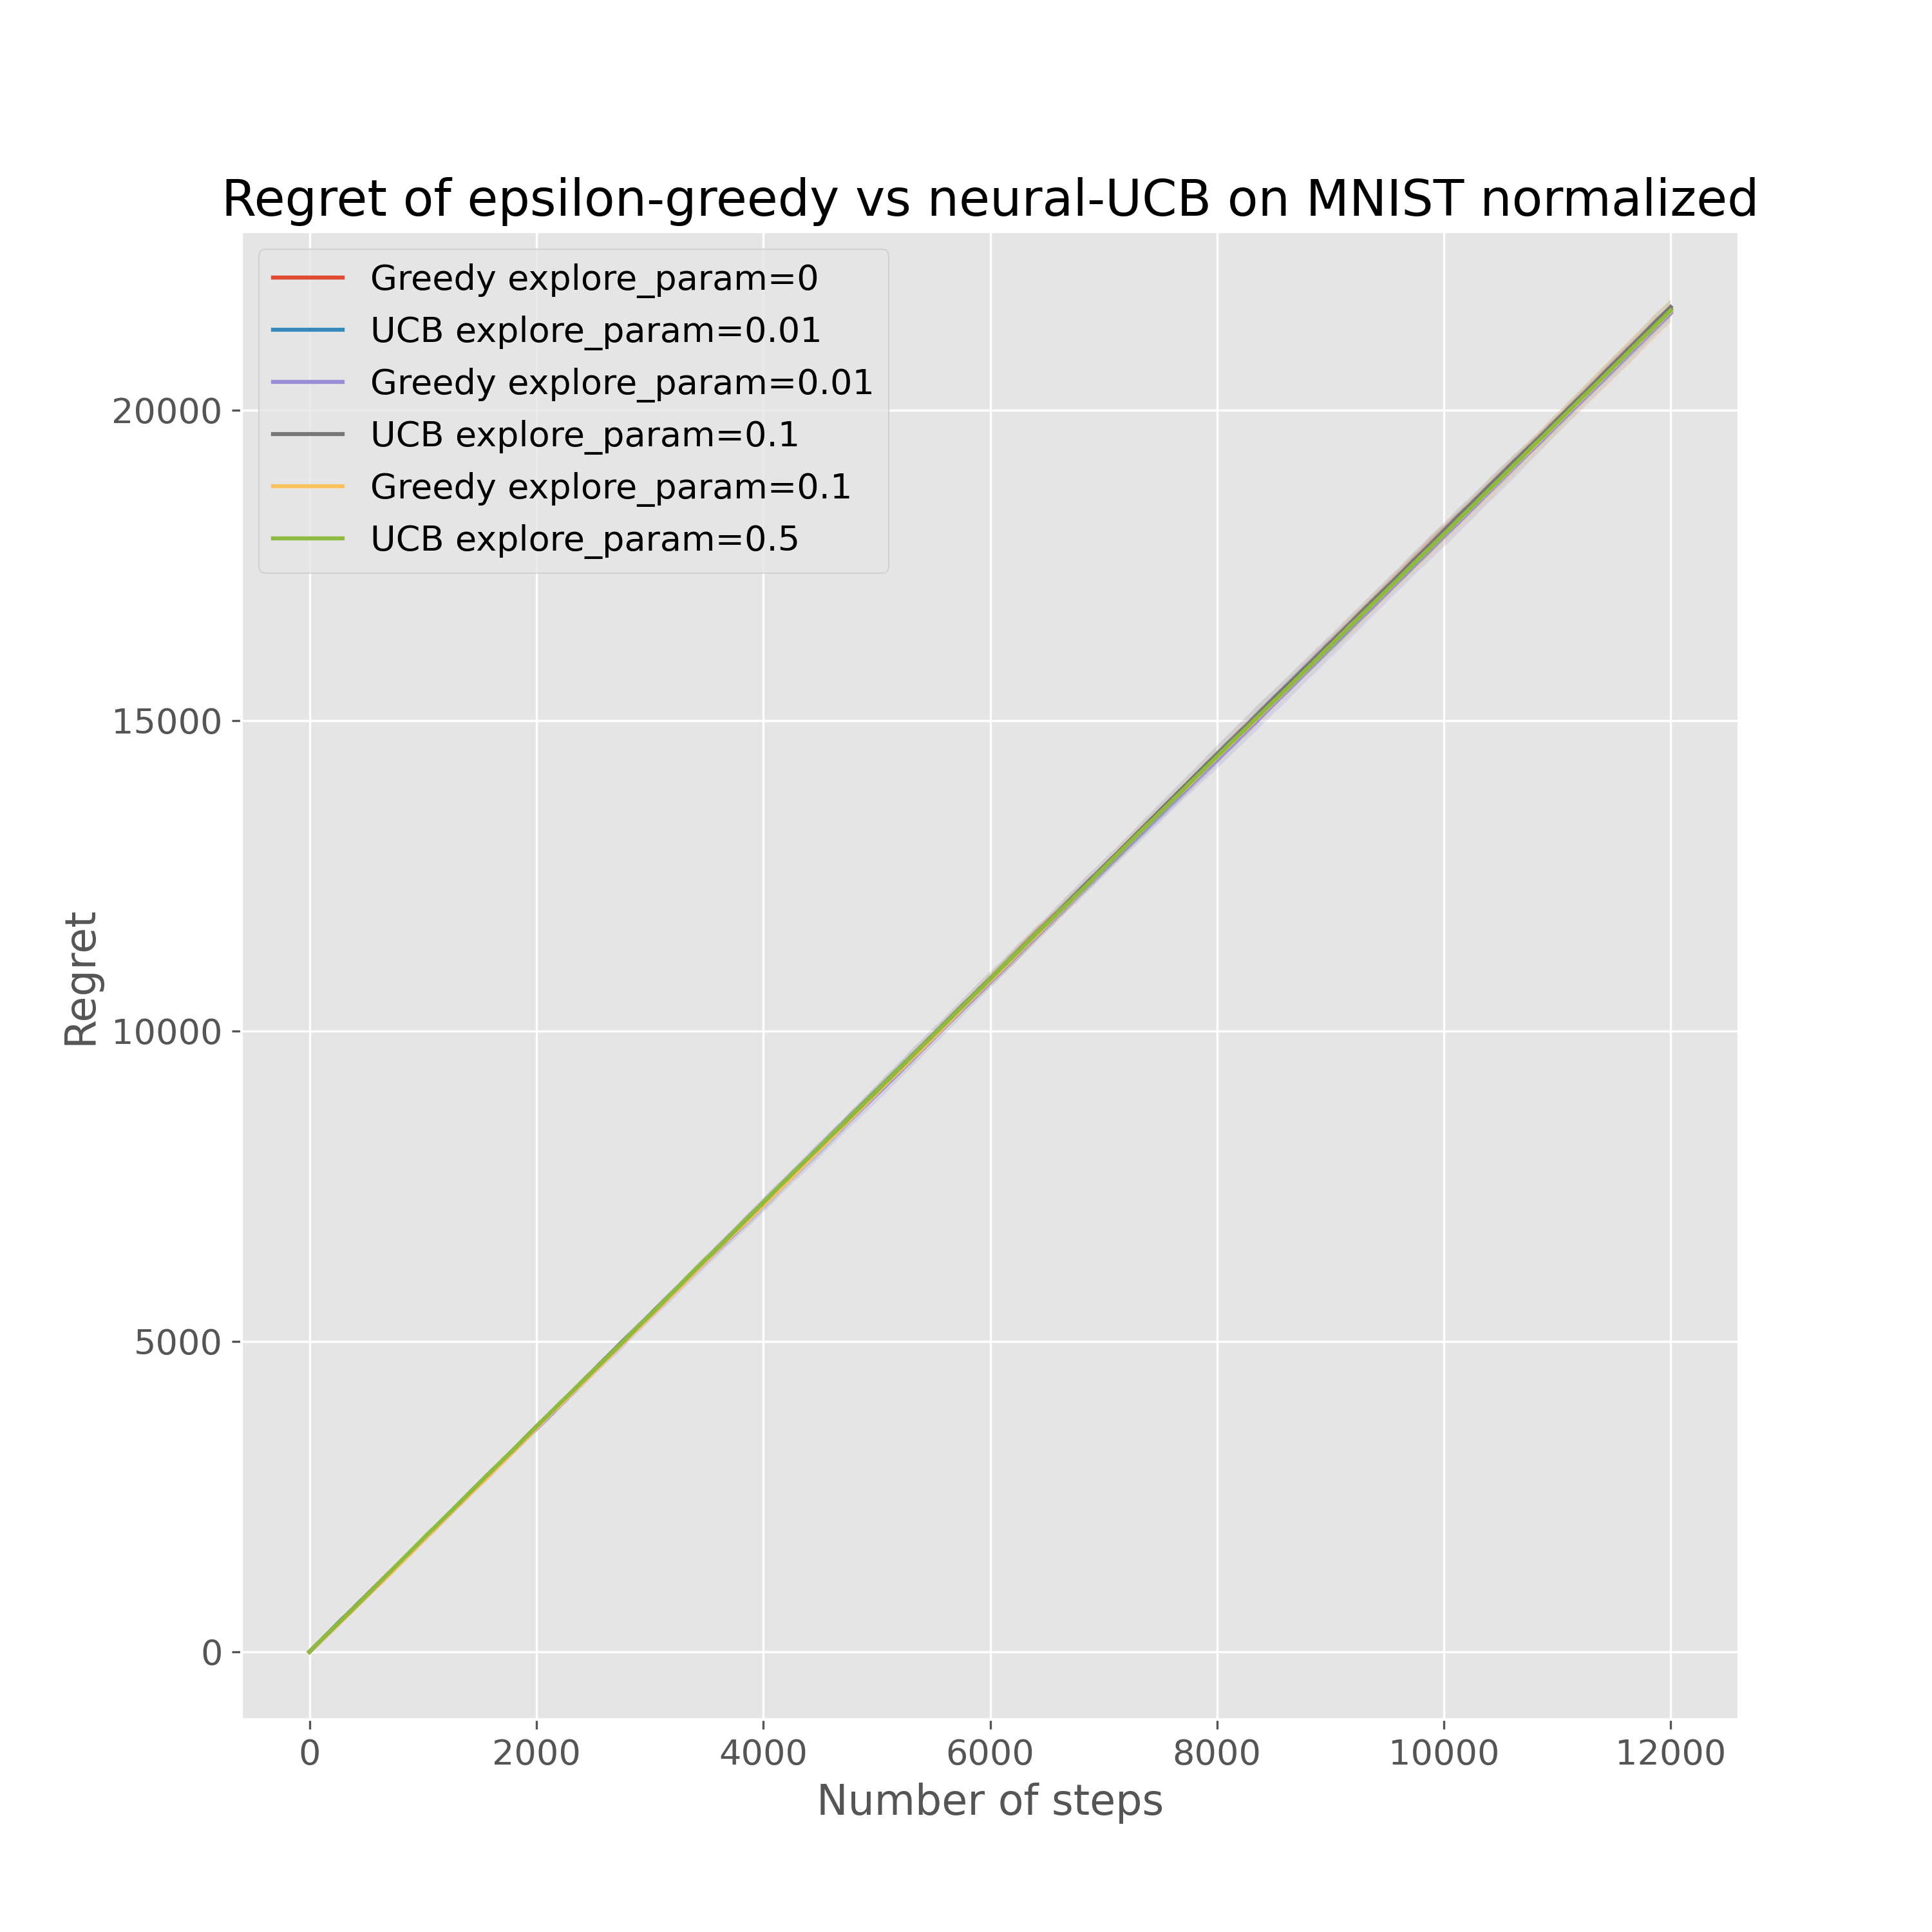
\includegraphics[width=\linewidth]{online-epsilon-vs-neural-mnist--normalized-ci}
  \end{minipage}
  \caption{Performance OnSim-NeuralUCB on non-normalized and normalized features}\label{fig:online-epsilon-vs-neural-ci-mnist}
\end{figure}


\end{document}
